% Step 01: start_task, reset, noop x12, click(2,2), noop x3, click(3,2), noop x3, click(3,3), noop x3, click(4,3), noop x3, right, noop x3, click(5,2), noop x3, click(5,1), noop x3, click(5,0), noop x2
\smallskip
\newcount\ActionSequenceCounter

\newcommand{\ActionSequence}[1]{%
  \begingroup
  \ActionSequenceCounter=0\relax
  \def\ActionsLabel{\textit{Actions: }}%
  \par\noindent\ActionsLabel%
  #1\relax
  \par\endgroup
}

\newcommand{\ActionItem}[1]{%
  \ifnum\ActionSequenceCounter>0\relax
    \ifnum\ActionSequenceCounter=4\relax
      \ActionSequenceCounter=0\relax
      \newline\phantom{\ActionsLabel}#1%
    \else
      \,\texttt{->}\,#1%
    \fi
  \else
    #1%
  \fi
  \advance\ActionSequenceCounter by 1\relax
}

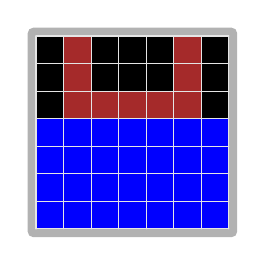
\begin{tikzpicture}
% TikZ grid exported from MARA
\def\cellsz{0.35cm}
\providecommand{\maraGridLineColor}{black!10}
\providecommand{\maraGridBorderColor}{black!30}
\providecommand{\maraGridLineWidth}{0.4pt}
\providecommand{\maraBorderLineWidth}{3pt}
\providecommand{\maraBorderRadius}{2pt}
\begin{scope}[x=\cellsz, y=\cellsz, line cap=round, line join=round]
  % Outer frame as a filled ring expanded by border line width with rounded corners
  \path[fill=\maraGridBorderColor, rounded corners=\maraBorderRadius] ([xshift=-\maraBorderLineWidth,yshift=-\maraBorderLineWidth]0,0) rectangle ([xshift=\maraBorderLineWidth,yshift=\maraBorderLineWidth]7,7);
  % Background
  \fill[black] (0,0) rectangle (7,7);
  % Filled cells
  \begin{scope}[fill={rgb,1:red,0.647;green,0.165;blue,0.165}, fill opacity=1.000]
    \fill (1,6) rectangle ++(1,1);
    \fill (5,6) rectangle ++(1,1);
    \fill (1,5) rectangle ++(1,1);
    \fill (5,5) rectangle ++(1,1);
    \fill (1,4) rectangle ++(1,1);
    \fill (2,4) rectangle ++(1,1);
    \fill (3,4) rectangle ++(1,1);
    \fill (4,4) rectangle ++(1,1);
    \fill (5,4) rectangle ++(1,1);
  \end{scope}
  \begin{scope}[fill={rgb,1:red,0.000;green,0.000;blue,1.000}, fill opacity=1.000]
    \fill (0,3) rectangle ++(1,1);
    \fill (1,3) rectangle ++(1,1);
    \fill (2,3) rectangle ++(1,1);
    \fill (3,3) rectangle ++(1,1);
    \fill (4,3) rectangle ++(1,1);
    \fill (5,3) rectangle ++(1,1);
    \fill (6,3) rectangle ++(1,1);
    \fill (0,2) rectangle ++(1,1);
    \fill (1,2) rectangle ++(1,1);
    \fill (2,2) rectangle ++(1,1);
    \fill (3,2) rectangle ++(1,1);
    \fill (4,2) rectangle ++(1,1);
    \fill (5,2) rectangle ++(1,1);
    \fill (6,2) rectangle ++(1,1);
    \fill (0,1) rectangle ++(1,1);
    \fill (1,1) rectangle ++(1,1);
    \fill (2,1) rectangle ++(1,1);
    \fill (3,1) rectangle ++(1,1);
    \fill (4,1) rectangle ++(1,1);
    \fill (5,1) rectangle ++(1,1);
    \fill (6,1) rectangle ++(1,1);
    \fill (0,0) rectangle ++(1,1);
    \fill (1,0) rectangle ++(1,1);
    \fill (2,0) rectangle ++(1,1);
    \fill (3,0) rectangle ++(1,1);
    \fill (4,0) rectangle ++(1,1);
    \fill (5,0) rectangle ++(1,1);
    \fill (6,0) rectangle ++(1,1);
  \end{scope}
  % Grid and outline
  % Vertical lines
  \begin{scope}[draw=\maraGridLineColor, line width=\maraGridLineWidth, line cap=round]
    \draw (0,0) -- (0,7);
    \draw (1,0) -- (1,7);
    \draw (2,0) -- (2,7);
    \draw (3,0) -- (3,7);
    \draw (4,0) -- (4,7);
    \draw (5,0) -- (5,7);
    \draw (6,0) -- (6,7);
    \draw (7,0) -- (7,7);
  \end{scope}
  % Horizontal lines
  \begin{scope}[draw=\maraGridLineColor, line width=\maraGridLineWidth, line cap=round]
    \draw (0,0) -- (7,0);
    \draw (0,1) -- (7,1);
    \draw (0,2) -- (7,2);
    \draw (0,3) -- (7,3);
    \draw (0,4) -- (7,4);
    \draw (0,5) -- (7,5);
    \draw (0,6) -- (7,6);
    \draw (0,7) -- (7,7);
  \end{scope}
\end{scope}
\end{tikzpicture}
\ActionSequence{\ActionItem{start_task}\ActionItem{reset}\ActionItem{noop x12}\ActionItem{click(2,2)}\ActionItem{noop x3}\ActionItem{click(3,2)}\ActionItem{noop x3}\ActionItem{click(3,3)}\ActionItem{noop x3}\ActionItem{click(4,3)}\ActionItem{noop x3}\ActionItem{right}\ActionItem{noop x3}\ActionItem{click(5,2)}\ActionItem{noop x3}\ActionItem{click(5,1)}\ActionItem{noop x3}\ActionItem{click(5,0)}\ActionItem{noop x2}}
\medskip
% Step 02: click(4,0)
\smallskip
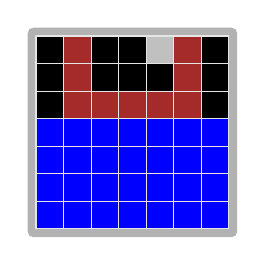
\begin{tikzpicture}
% TikZ grid exported from MARA
\def\cellsz{0.35cm}
\providecommand{\maraGridLineColor}{black!10}
\providecommand{\maraGridBorderColor}{black!30}
\providecommand{\maraGridLineWidth}{0.4pt}
\providecommand{\maraBorderLineWidth}{3pt}
\providecommand{\maraBorderRadius}{2pt}
\begin{scope}[x=\cellsz, y=\cellsz, line cap=round, line join=round]
  % Outer frame as a filled ring expanded by border line width with rounded corners
  \path[fill=\maraGridBorderColor, rounded corners=\maraBorderRadius] ([xshift=-\maraBorderLineWidth,yshift=-\maraBorderLineWidth]0,0) rectangle ([xshift=\maraBorderLineWidth,yshift=\maraBorderLineWidth]7,7);
  % Background
  \fill[black] (0,0) rectangle (7,7);
  % Filled cells
  \begin{scope}[fill={rgb,1:red,0.647;green,0.165;blue,0.165}, fill opacity=1.000]
    \fill (1,6) rectangle ++(1,1);
    \fill (5,6) rectangle ++(1,1);
    \fill (1,5) rectangle ++(1,1);
    \fill (5,5) rectangle ++(1,1);
    \fill (1,4) rectangle ++(1,1);
    \fill (2,4) rectangle ++(1,1);
    \fill (3,4) rectangle ++(1,1);
    \fill (4,4) rectangle ++(1,1);
    \fill (5,4) rectangle ++(1,1);
  \end{scope}
  \begin{scope}[fill={rgb,1:red,0.753;green,0.753;blue,0.753}, fill opacity=1.000]
    \fill (4,6) rectangle ++(1,1);
  \end{scope}
  \begin{scope}[fill={rgb,1:red,0.000;green,0.000;blue,1.000}, fill opacity=1.000]
    \fill (0,3) rectangle ++(1,1);
    \fill (1,3) rectangle ++(1,1);
    \fill (2,3) rectangle ++(1,1);
    \fill (3,3) rectangle ++(1,1);
    \fill (4,3) rectangle ++(1,1);
    \fill (5,3) rectangle ++(1,1);
    \fill (6,3) rectangle ++(1,1);
    \fill (0,2) rectangle ++(1,1);
    \fill (1,2) rectangle ++(1,1);
    \fill (2,2) rectangle ++(1,1);
    \fill (3,2) rectangle ++(1,1);
    \fill (4,2) rectangle ++(1,1);
    \fill (5,2) rectangle ++(1,1);
    \fill (6,2) rectangle ++(1,1);
    \fill (0,1) rectangle ++(1,1);
    \fill (1,1) rectangle ++(1,1);
    \fill (2,1) rectangle ++(1,1);
    \fill (3,1) rectangle ++(1,1);
    \fill (4,1) rectangle ++(1,1);
    \fill (5,1) rectangle ++(1,1);
    \fill (6,1) rectangle ++(1,1);
    \fill (0,0) rectangle ++(1,1);
    \fill (1,0) rectangle ++(1,1);
    \fill (2,0) rectangle ++(1,1);
    \fill (3,0) rectangle ++(1,1);
    \fill (4,0) rectangle ++(1,1);
    \fill (5,0) rectangle ++(1,1);
    \fill (6,0) rectangle ++(1,1);
  \end{scope}
  % Grid and outline
  % Vertical lines
  \begin{scope}[draw=\maraGridLineColor, line width=\maraGridLineWidth, line cap=round]
    \draw (0,0) -- (0,7);
    \draw (1,0) -- (1,7);
    \draw (2,0) -- (2,7);
    \draw (3,0) -- (3,7);
    \draw (4,0) -- (4,7);
    \draw (5,0) -- (5,7);
    \draw (6,0) -- (6,7);
    \draw (7,0) -- (7,7);
  \end{scope}
  % Horizontal lines
  \begin{scope}[draw=\maraGridLineColor, line width=\maraGridLineWidth, line cap=round]
    \draw (0,0) -- (7,0);
    \draw (0,1) -- (7,1);
    \draw (0,2) -- (7,2);
    \draw (0,3) -- (7,3);
    \draw (0,4) -- (7,4);
    \draw (0,5) -- (7,5);
    \draw (0,6) -- (7,6);
    \draw (0,7) -- (7,7);
  \end{scope}
\end{scope}
\end{tikzpicture}
\ActionSequence{\ActionItem{click(4,0)}}
\medskip
% Step 03: noop x1
\smallskip
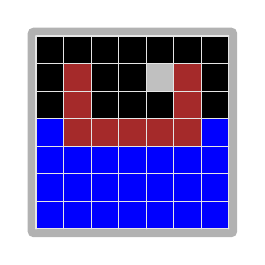
\begin{tikzpicture}
% TikZ grid exported from MARA
\def\cellsz{0.35cm}
\providecommand{\maraGridLineColor}{black!10}
\providecommand{\maraGridBorderColor}{black!30}
\providecommand{\maraGridLineWidth}{0.4pt}
\providecommand{\maraBorderLineWidth}{3pt}
\providecommand{\maraBorderRadius}{2pt}
\begin{scope}[x=\cellsz, y=\cellsz, line cap=round, line join=round]
  % Outer frame as a filled ring expanded by border line width with rounded corners
  \path[fill=\maraGridBorderColor, rounded corners=\maraBorderRadius] ([xshift=-\maraBorderLineWidth,yshift=-\maraBorderLineWidth]0,0) rectangle ([xshift=\maraBorderLineWidth,yshift=\maraBorderLineWidth]7,7);
  % Background
  \fill[black] (0,0) rectangle (7,7);
  % Filled cells
  \begin{scope}[fill={rgb,1:red,0.647;green,0.165;blue,0.165}, fill opacity=1.000]
    \fill (1,5) rectangle ++(1,1);
    \fill (5,5) rectangle ++(1,1);
    \fill (1,4) rectangle ++(1,1);
    \fill (5,4) rectangle ++(1,1);
    \fill (1,3) rectangle ++(1,1);
    \fill (2,3) rectangle ++(1,1);
    \fill (3,3) rectangle ++(1,1);
    \fill (4,3) rectangle ++(1,1);
    \fill (5,3) rectangle ++(1,1);
  \end{scope}
  \begin{scope}[fill={rgb,1:red,0.753;green,0.753;blue,0.753}, fill opacity=1.000]
    \fill (4,5) rectangle ++(1,1);
  \end{scope}
  \begin{scope}[fill={rgb,1:red,0.000;green,0.000;blue,1.000}, fill opacity=1.000]
    \fill (0,3) rectangle ++(1,1);
    \fill (6,3) rectangle ++(1,1);
    \fill (0,2) rectangle ++(1,1);
    \fill (1,2) rectangle ++(1,1);
    \fill (2,2) rectangle ++(1,1);
    \fill (3,2) rectangle ++(1,1);
    \fill (4,2) rectangle ++(1,1);
    \fill (5,2) rectangle ++(1,1);
    \fill (6,2) rectangle ++(1,1);
    \fill (0,1) rectangle ++(1,1);
    \fill (1,1) rectangle ++(1,1);
    \fill (2,1) rectangle ++(1,1);
    \fill (3,1) rectangle ++(1,1);
    \fill (4,1) rectangle ++(1,1);
    \fill (5,1) rectangle ++(1,1);
    \fill (6,1) rectangle ++(1,1);
    \fill (0,0) rectangle ++(1,1);
    \fill (1,0) rectangle ++(1,1);
    \fill (2,0) rectangle ++(1,1);
    \fill (3,0) rectangle ++(1,1);
    \fill (4,0) rectangle ++(1,1);
    \fill (5,0) rectangle ++(1,1);
    \fill (6,0) rectangle ++(1,1);
  \end{scope}
  % Grid and outline
  % Vertical lines
  \begin{scope}[draw=\maraGridLineColor, line width=\maraGridLineWidth, line cap=round]
    \draw (0,0) -- (0,7);
    \draw (1,0) -- (1,7);
    \draw (2,0) -- (2,7);
    \draw (3,0) -- (3,7);
    \draw (4,0) -- (4,7);
    \draw (5,0) -- (5,7);
    \draw (6,0) -- (6,7);
    \draw (7,0) -- (7,7);
  \end{scope}
  % Horizontal lines
  \begin{scope}[draw=\maraGridLineColor, line width=\maraGridLineWidth, line cap=round]
    \draw (0,0) -- (7,0);
    \draw (0,1) -- (7,1);
    \draw (0,2) -- (7,2);
    \draw (0,3) -- (7,3);
    \draw (0,4) -- (7,4);
    \draw (0,5) -- (7,5);
    \draw (0,6) -- (7,6);
    \draw (0,7) -- (7,7);
  \end{scope}
\end{scope}
\end{tikzpicture}
\ActionSequence{\ActionItem{noop x1}}
\medskip
% Step 04: noop x16
\smallskip
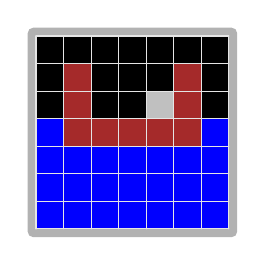
\begin{tikzpicture}
% TikZ grid exported from MARA
\def\cellsz{0.35cm}
\providecommand{\maraGridLineColor}{black!10}
\providecommand{\maraGridBorderColor}{black!30}
\providecommand{\maraGridLineWidth}{0.4pt}
\providecommand{\maraBorderLineWidth}{3pt}
\providecommand{\maraBorderRadius}{2pt}
\begin{scope}[x=\cellsz, y=\cellsz, line cap=round, line join=round]
  % Outer frame as a filled ring expanded by border line width with rounded corners
  \path[fill=\maraGridBorderColor, rounded corners=\maraBorderRadius] ([xshift=-\maraBorderLineWidth,yshift=-\maraBorderLineWidth]0,0) rectangle ([xshift=\maraBorderLineWidth,yshift=\maraBorderLineWidth]7,7);
  % Background
  \fill[black] (0,0) rectangle (7,7);
  % Filled cells
  \begin{scope}[fill={rgb,1:red,0.647;green,0.165;blue,0.165}, fill opacity=1.000]
    \fill (1,5) rectangle ++(1,1);
    \fill (5,5) rectangle ++(1,1);
    \fill (1,4) rectangle ++(1,1);
    \fill (5,4) rectangle ++(1,1);
    \fill (1,3) rectangle ++(1,1);
    \fill (2,3) rectangle ++(1,1);
    \fill (3,3) rectangle ++(1,1);
    \fill (4,3) rectangle ++(1,1);
    \fill (5,3) rectangle ++(1,1);
  \end{scope}
  \begin{scope}[fill={rgb,1:red,0.753;green,0.753;blue,0.753}, fill opacity=1.000]
    \fill (4,4) rectangle ++(1,1);
  \end{scope}
  \begin{scope}[fill={rgb,1:red,0.000;green,0.000;blue,1.000}, fill opacity=1.000]
    \fill (0,3) rectangle ++(1,1);
    \fill (6,3) rectangle ++(1,1);
    \fill (0,2) rectangle ++(1,1);
    \fill (1,2) rectangle ++(1,1);
    \fill (2,2) rectangle ++(1,1);
    \fill (3,2) rectangle ++(1,1);
    \fill (4,2) rectangle ++(1,1);
    \fill (5,2) rectangle ++(1,1);
    \fill (6,2) rectangle ++(1,1);
    \fill (0,1) rectangle ++(1,1);
    \fill (1,1) rectangle ++(1,1);
    \fill (2,1) rectangle ++(1,1);
    \fill (3,1) rectangle ++(1,1);
    \fill (4,1) rectangle ++(1,1);
    \fill (5,1) rectangle ++(1,1);
    \fill (6,1) rectangle ++(1,1);
    \fill (0,0) rectangle ++(1,1);
    \fill (1,0) rectangle ++(1,1);
    \fill (2,0) rectangle ++(1,1);
    \fill (3,0) rectangle ++(1,1);
    \fill (4,0) rectangle ++(1,1);
    \fill (5,0) rectangle ++(1,1);
    \fill (6,0) rectangle ++(1,1);
  \end{scope}
  % Grid and outline
  % Vertical lines
  \begin{scope}[draw=\maraGridLineColor, line width=\maraGridLineWidth, line cap=round]
    \draw (0,0) -- (0,7);
    \draw (1,0) -- (1,7);
    \draw (2,0) -- (2,7);
    \draw (3,0) -- (3,7);
    \draw (4,0) -- (4,7);
    \draw (5,0) -- (5,7);
    \draw (6,0) -- (6,7);
    \draw (7,0) -- (7,7);
  \end{scope}
  % Horizontal lines
  \begin{scope}[draw=\maraGridLineColor, line width=\maraGridLineWidth, line cap=round]
    \draw (0,0) -- (7,0);
    \draw (0,1) -- (7,1);
    \draw (0,2) -- (7,2);
    \draw (0,3) -- (7,3);
    \draw (0,4) -- (7,4);
    \draw (0,5) -- (7,5);
    \draw (0,6) -- (7,6);
    \draw (0,7) -- (7,7);
  \end{scope}
\end{scope}
\end{tikzpicture}
\ActionSequence{\ActionItem{noop x16}}
\medskip
% Step 05: click(3,2)
\smallskip
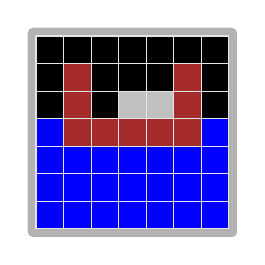
\begin{tikzpicture}
% TikZ grid exported from MARA
\def\cellsz{0.35cm}
\providecommand{\maraGridLineColor}{black!10}
\providecommand{\maraGridBorderColor}{black!30}
\providecommand{\maraGridLineWidth}{0.4pt}
\providecommand{\maraBorderLineWidth}{3pt}
\providecommand{\maraBorderRadius}{2pt}
\begin{scope}[x=\cellsz, y=\cellsz, line cap=round, line join=round]
  % Outer frame as a filled ring expanded by border line width with rounded corners
  \path[fill=\maraGridBorderColor, rounded corners=\maraBorderRadius] ([xshift=-\maraBorderLineWidth,yshift=-\maraBorderLineWidth]0,0) rectangle ([xshift=\maraBorderLineWidth,yshift=\maraBorderLineWidth]7,7);
  % Background
  \fill[black] (0,0) rectangle (7,7);
  % Filled cells
  \begin{scope}[fill={rgb,1:red,0.647;green,0.165;blue,0.165}, fill opacity=1.000]
    \fill (1,5) rectangle ++(1,1);
    \fill (5,5) rectangle ++(1,1);
    \fill (1,4) rectangle ++(1,1);
    \fill (5,4) rectangle ++(1,1);
    \fill (1,3) rectangle ++(1,1);
    \fill (2,3) rectangle ++(1,1);
    \fill (3,3) rectangle ++(1,1);
    \fill (4,3) rectangle ++(1,1);
    \fill (5,3) rectangle ++(1,1);
  \end{scope}
  \begin{scope}[fill={rgb,1:red,0.753;green,0.753;blue,0.753}, fill opacity=1.000]
    \fill (3,4) rectangle ++(1,1);
    \fill (4,4) rectangle ++(1,1);
  \end{scope}
  \begin{scope}[fill={rgb,1:red,0.000;green,0.000;blue,1.000}, fill opacity=1.000]
    \fill (0,3) rectangle ++(1,1);
    \fill (6,3) rectangle ++(1,1);
    \fill (0,2) rectangle ++(1,1);
    \fill (1,2) rectangle ++(1,1);
    \fill (2,2) rectangle ++(1,1);
    \fill (3,2) rectangle ++(1,1);
    \fill (4,2) rectangle ++(1,1);
    \fill (5,2) rectangle ++(1,1);
    \fill (6,2) rectangle ++(1,1);
    \fill (0,1) rectangle ++(1,1);
    \fill (1,1) rectangle ++(1,1);
    \fill (2,1) rectangle ++(1,1);
    \fill (3,1) rectangle ++(1,1);
    \fill (4,1) rectangle ++(1,1);
    \fill (5,1) rectangle ++(1,1);
    \fill (6,1) rectangle ++(1,1);
    \fill (0,0) rectangle ++(1,1);
    \fill (1,0) rectangle ++(1,1);
    \fill (2,0) rectangle ++(1,1);
    \fill (3,0) rectangle ++(1,1);
    \fill (4,0) rectangle ++(1,1);
    \fill (5,0) rectangle ++(1,1);
    \fill (6,0) rectangle ++(1,1);
  \end{scope}
  % Grid and outline
  % Vertical lines
  \begin{scope}[draw=\maraGridLineColor, line width=\maraGridLineWidth, line cap=round]
    \draw (0,0) -- (0,7);
    \draw (1,0) -- (1,7);
    \draw (2,0) -- (2,7);
    \draw (3,0) -- (3,7);
    \draw (4,0) -- (4,7);
    \draw (5,0) -- (5,7);
    \draw (6,0) -- (6,7);
    \draw (7,0) -- (7,7);
  \end{scope}
  % Horizontal lines
  \begin{scope}[draw=\maraGridLineColor, line width=\maraGridLineWidth, line cap=round]
    \draw (0,0) -- (7,0);
    \draw (0,1) -- (7,1);
    \draw (0,2) -- (7,2);
    \draw (0,3) -- (7,3);
    \draw (0,4) -- (7,4);
    \draw (0,5) -- (7,5);
    \draw (0,6) -- (7,6);
    \draw (0,7) -- (7,7);
  \end{scope}
\end{scope}
\end{tikzpicture}
\ActionSequence{\ActionItem{click(3,2)}}
\medskip
% Step 06: noop x9
\smallskip
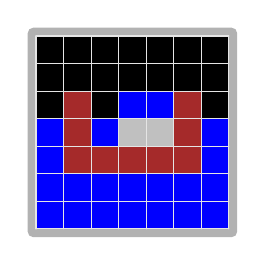
\begin{tikzpicture}
% TikZ grid exported from MARA
\def\cellsz{0.35cm}
\providecommand{\maraGridLineColor}{black!10}
\providecommand{\maraGridBorderColor}{black!30}
\providecommand{\maraGridLineWidth}{0.4pt}
\providecommand{\maraBorderLineWidth}{3pt}
\providecommand{\maraBorderRadius}{2pt}
\begin{scope}[x=\cellsz, y=\cellsz, line cap=round, line join=round]
  % Outer frame as a filled ring expanded by border line width with rounded corners
  \path[fill=\maraGridBorderColor, rounded corners=\maraBorderRadius] ([xshift=-\maraBorderLineWidth,yshift=-\maraBorderLineWidth]0,0) rectangle ([xshift=\maraBorderLineWidth,yshift=\maraBorderLineWidth]7,7);
  % Background
  \fill[black] (0,0) rectangle (7,7);
  % Filled cells
  \begin{scope}[fill={rgb,1:red,0.647;green,0.165;blue,0.165}, fill opacity=1.000]
    \fill (1,4) rectangle ++(1,1);
    \fill (5,4) rectangle ++(1,1);
    \fill (1,3) rectangle ++(1,1);
    \fill (5,3) rectangle ++(1,1);
    \fill (1,2) rectangle ++(1,1);
    \fill (2,2) rectangle ++(1,1);
    \fill (3,2) rectangle ++(1,1);
    \fill (4,2) rectangle ++(1,1);
    \fill (5,2) rectangle ++(1,1);
  \end{scope}
  \begin{scope}[fill={rgb,1:red,0.000;green,0.000;blue,1.000}, fill opacity=1.000]
    \fill (3,4) rectangle ++(1,1);
    \fill (4,4) rectangle ++(1,1);
    \fill (0,3) rectangle ++(1,1);
    \fill (2,3) rectangle ++(1,1);
    \fill (6,3) rectangle ++(1,1);
    \fill (0,2) rectangle ++(1,1);
    \fill (6,2) rectangle ++(1,1);
    \fill (0,1) rectangle ++(1,1);
    \fill (1,1) rectangle ++(1,1);
    \fill (2,1) rectangle ++(1,1);
    \fill (3,1) rectangle ++(1,1);
    \fill (4,1) rectangle ++(1,1);
    \fill (5,1) rectangle ++(1,1);
    \fill (6,1) rectangle ++(1,1);
    \fill (0,0) rectangle ++(1,1);
    \fill (1,0) rectangle ++(1,1);
    \fill (2,0) rectangle ++(1,1);
    \fill (3,0) rectangle ++(1,1);
    \fill (4,0) rectangle ++(1,1);
    \fill (5,0) rectangle ++(1,1);
    \fill (6,0) rectangle ++(1,1);
  \end{scope}
  \begin{scope}[fill={rgb,1:red,0.753;green,0.753;blue,0.753}, fill opacity=1.000]
    \fill (3,3) rectangle ++(1,1);
    \fill (4,3) rectangle ++(1,1);
  \end{scope}
  % Grid and outline
  % Vertical lines
  \begin{scope}[draw=\maraGridLineColor, line width=\maraGridLineWidth, line cap=round]
    \draw (0,0) -- (0,7);
    \draw (1,0) -- (1,7);
    \draw (2,0) -- (2,7);
    \draw (3,0) -- (3,7);
    \draw (4,0) -- (4,7);
    \draw (5,0) -- (5,7);
    \draw (6,0) -- (6,7);
    \draw (7,0) -- (7,7);
  \end{scope}
  % Horizontal lines
  \begin{scope}[draw=\maraGridLineColor, line width=\maraGridLineWidth, line cap=round]
    \draw (0,0) -- (7,0);
    \draw (0,1) -- (7,1);
    \draw (0,2) -- (7,2);
    \draw (0,3) -- (7,3);
    \draw (0,4) -- (7,4);
    \draw (0,5) -- (7,5);
    \draw (0,6) -- (7,6);
    \draw (0,7) -- (7,7);
  \end{scope}
\end{scope}
\end{tikzpicture}
\ActionSequence{\ActionItem{noop x9}}
\medskip
% Step 07: click(2,2)
\smallskip
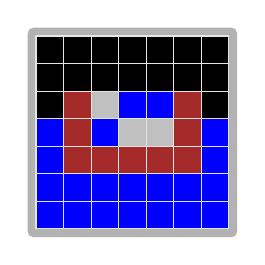
\begin{tikzpicture}
% TikZ grid exported from MARA
\def\cellsz{0.35cm}
\providecommand{\maraGridLineColor}{black!10}
\providecommand{\maraGridBorderColor}{black!30}
\providecommand{\maraGridLineWidth}{0.4pt}
\providecommand{\maraBorderLineWidth}{3pt}
\providecommand{\maraBorderRadius}{2pt}
\begin{scope}[x=\cellsz, y=\cellsz, line cap=round, line join=round]
  % Outer frame as a filled ring expanded by border line width with rounded corners
  \path[fill=\maraGridBorderColor, rounded corners=\maraBorderRadius] ([xshift=-\maraBorderLineWidth,yshift=-\maraBorderLineWidth]0,0) rectangle ([xshift=\maraBorderLineWidth,yshift=\maraBorderLineWidth]7,7);
  % Background
  \fill[black] (0,0) rectangle (7,7);
  % Filled cells
  \begin{scope}[fill={rgb,1:red,0.647;green,0.165;blue,0.165}, fill opacity=1.000]
    \fill (1,4) rectangle ++(1,1);
    \fill (5,4) rectangle ++(1,1);
    \fill (1,3) rectangle ++(1,1);
    \fill (5,3) rectangle ++(1,1);
    \fill (1,2) rectangle ++(1,1);
    \fill (2,2) rectangle ++(1,1);
    \fill (3,2) rectangle ++(1,1);
    \fill (4,2) rectangle ++(1,1);
    \fill (5,2) rectangle ++(1,1);
  \end{scope}
  \begin{scope}[fill={rgb,1:red,0.753;green,0.753;blue,0.753}, fill opacity=1.000]
    \fill (2,4) rectangle ++(1,1);
    \fill (3,3) rectangle ++(1,1);
    \fill (4,3) rectangle ++(1,1);
  \end{scope}
  \begin{scope}[fill={rgb,1:red,0.000;green,0.000;blue,1.000}, fill opacity=1.000]
    \fill (3,4) rectangle ++(1,1);
    \fill (4,4) rectangle ++(1,1);
    \fill (0,3) rectangle ++(1,1);
    \fill (2,3) rectangle ++(1,1);
    \fill (6,3) rectangle ++(1,1);
    \fill (0,2) rectangle ++(1,1);
    \fill (6,2) rectangle ++(1,1);
    \fill (0,1) rectangle ++(1,1);
    \fill (1,1) rectangle ++(1,1);
    \fill (2,1) rectangle ++(1,1);
    \fill (3,1) rectangle ++(1,1);
    \fill (4,1) rectangle ++(1,1);
    \fill (5,1) rectangle ++(1,1);
    \fill (6,1) rectangle ++(1,1);
    \fill (0,0) rectangle ++(1,1);
    \fill (1,0) rectangle ++(1,1);
    \fill (2,0) rectangle ++(1,1);
    \fill (3,0) rectangle ++(1,1);
    \fill (4,0) rectangle ++(1,1);
    \fill (5,0) rectangle ++(1,1);
    \fill (6,0) rectangle ++(1,1);
  \end{scope}
  % Grid and outline
  % Vertical lines
  \begin{scope}[draw=\maraGridLineColor, line width=\maraGridLineWidth, line cap=round]
    \draw (0,0) -- (0,7);
    \draw (1,0) -- (1,7);
    \draw (2,0) -- (2,7);
    \draw (3,0) -- (3,7);
    \draw (4,0) -- (4,7);
    \draw (5,0) -- (5,7);
    \draw (6,0) -- (6,7);
    \draw (7,0) -- (7,7);
  \end{scope}
  % Horizontal lines
  \begin{scope}[draw=\maraGridLineColor, line width=\maraGridLineWidth, line cap=round]
    \draw (0,0) -- (7,0);
    \draw (0,1) -- (7,1);
    \draw (0,2) -- (7,2);
    \draw (0,3) -- (7,3);
    \draw (0,4) -- (7,4);
    \draw (0,5) -- (7,5);
    \draw (0,6) -- (7,6);
    \draw (0,7) -- (7,7);
  \end{scope}
\end{scope}
\end{tikzpicture}
\ActionSequence{\ActionItem{click(2,2)}}
\medskip
% Step 08: noop x1
\smallskip
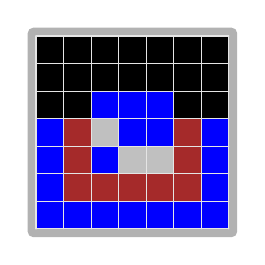
\begin{tikzpicture}
% TikZ grid exported from MARA
\def\cellsz{0.35cm}
\providecommand{\maraGridLineColor}{black!10}
\providecommand{\maraGridBorderColor}{black!30}
\providecommand{\maraGridLineWidth}{0.4pt}
\providecommand{\maraBorderLineWidth}{3pt}
\providecommand{\maraBorderRadius}{2pt}
\begin{scope}[x=\cellsz, y=\cellsz, line cap=round, line join=round]
  % Outer frame as a filled ring expanded by border line width with rounded corners
  \path[fill=\maraGridBorderColor, rounded corners=\maraBorderRadius] ([xshift=-\maraBorderLineWidth,yshift=-\maraBorderLineWidth]0,0) rectangle ([xshift=\maraBorderLineWidth,yshift=\maraBorderLineWidth]7,7);
  % Background
  \fill[black] (0,0) rectangle (7,7);
  % Filled cells
  \begin{scope}[fill={rgb,1:red,0.000;green,0.000;blue,1.000}, fill opacity=1.000]
    \fill (2,4) rectangle ++(1,1);
    \fill (3,4) rectangle ++(1,1);
    \fill (4,4) rectangle ++(1,1);
    \fill (0,3) rectangle ++(1,1);
    \fill (3,3) rectangle ++(1,1);
    \fill (4,3) rectangle ++(1,1);
    \fill (6,3) rectangle ++(1,1);
    \fill (0,2) rectangle ++(1,1);
    \fill (2,2) rectangle ++(1,1);
    \fill (6,2) rectangle ++(1,1);
    \fill (0,1) rectangle ++(1,1);
    \fill (6,1) rectangle ++(1,1);
    \fill (0,0) rectangle ++(1,1);
    \fill (1,0) rectangle ++(1,1);
    \fill (2,0) rectangle ++(1,1);
    \fill (3,0) rectangle ++(1,1);
    \fill (4,0) rectangle ++(1,1);
    \fill (5,0) rectangle ++(1,1);
    \fill (6,0) rectangle ++(1,1);
  \end{scope}
  \begin{scope}[fill={rgb,1:red,0.647;green,0.165;blue,0.165}, fill opacity=1.000]
    \fill (1,3) rectangle ++(1,1);
    \fill (5,3) rectangle ++(1,1);
    \fill (1,2) rectangle ++(1,1);
    \fill (5,2) rectangle ++(1,1);
    \fill (1,1) rectangle ++(1,1);
    \fill (2,1) rectangle ++(1,1);
    \fill (3,1) rectangle ++(1,1);
    \fill (4,1) rectangle ++(1,1);
    \fill (5,1) rectangle ++(1,1);
  \end{scope}
  \begin{scope}[fill={rgb,1:red,0.753;green,0.753;blue,0.753}, fill opacity=1.000]
    \fill (2,3) rectangle ++(1,1);
    \fill (3,2) rectangle ++(1,1);
    \fill (4,2) rectangle ++(1,1);
  \end{scope}
  % Grid and outline
  % Vertical lines
  \begin{scope}[draw=\maraGridLineColor, line width=\maraGridLineWidth, line cap=round]
    \draw (0,0) -- (0,7);
    \draw (1,0) -- (1,7);
    \draw (2,0) -- (2,7);
    \draw (3,0) -- (3,7);
    \draw (4,0) -- (4,7);
    \draw (5,0) -- (5,7);
    \draw (6,0) -- (6,7);
    \draw (7,0) -- (7,7);
  \end{scope}
  % Horizontal lines
  \begin{scope}[draw=\maraGridLineColor, line width=\maraGridLineWidth, line cap=round]
    \draw (0,0) -- (7,0);
    \draw (0,1) -- (7,1);
    \draw (0,2) -- (7,2);
    \draw (0,3) -- (7,3);
    \draw (0,4) -- (7,4);
    \draw (0,5) -- (7,5);
    \draw (0,6) -- (7,6);
    \draw (0,7) -- (7,7);
  \end{scope}
\end{scope}
\end{tikzpicture}
\ActionSequence{\ActionItem{noop x1}}
\medskip
% Step 09: noop x8
\smallskip
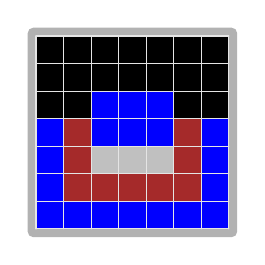
\begin{tikzpicture}
% TikZ grid exported from MARA
\def\cellsz{0.35cm}
\providecommand{\maraGridLineColor}{black!10}
\providecommand{\maraGridBorderColor}{black!30}
\providecommand{\maraGridLineWidth}{0.4pt}
\providecommand{\maraBorderLineWidth}{3pt}
\providecommand{\maraBorderRadius}{2pt}
\begin{scope}[x=\cellsz, y=\cellsz, line cap=round, line join=round]
  % Outer frame as a filled ring expanded by border line width with rounded corners
  \path[fill=\maraGridBorderColor, rounded corners=\maraBorderRadius] ([xshift=-\maraBorderLineWidth,yshift=-\maraBorderLineWidth]0,0) rectangle ([xshift=\maraBorderLineWidth,yshift=\maraBorderLineWidth]7,7);
  % Background
  \fill[black] (0,0) rectangle (7,7);
  % Filled cells
  \begin{scope}[fill={rgb,1:red,0.000;green,0.000;blue,1.000}, fill opacity=1.000]
    \fill (2,4) rectangle ++(1,1);
    \fill (3,4) rectangle ++(1,1);
    \fill (4,4) rectangle ++(1,1);
    \fill (0,3) rectangle ++(1,1);
    \fill (2,3) rectangle ++(1,1);
    \fill (3,3) rectangle ++(1,1);
    \fill (4,3) rectangle ++(1,1);
    \fill (6,3) rectangle ++(1,1);
    \fill (0,2) rectangle ++(1,1);
    \fill (6,2) rectangle ++(1,1);
    \fill (0,1) rectangle ++(1,1);
    \fill (6,1) rectangle ++(1,1);
    \fill (0,0) rectangle ++(1,1);
    \fill (1,0) rectangle ++(1,1);
    \fill (2,0) rectangle ++(1,1);
    \fill (3,0) rectangle ++(1,1);
    \fill (4,0) rectangle ++(1,1);
    \fill (5,0) rectangle ++(1,1);
    \fill (6,0) rectangle ++(1,1);
  \end{scope}
  \begin{scope}[fill={rgb,1:red,0.647;green,0.165;blue,0.165}, fill opacity=1.000]
    \fill (1,3) rectangle ++(1,1);
    \fill (5,3) rectangle ++(1,1);
    \fill (1,2) rectangle ++(1,1);
    \fill (5,2) rectangle ++(1,1);
    \fill (1,1) rectangle ++(1,1);
    \fill (2,1) rectangle ++(1,1);
    \fill (3,1) rectangle ++(1,1);
    \fill (4,1) rectangle ++(1,1);
    \fill (5,1) rectangle ++(1,1);
  \end{scope}
  \begin{scope}[fill={rgb,1:red,0.753;green,0.753;blue,0.753}, fill opacity=1.000]
    \fill (2,2) rectangle ++(1,1);
    \fill (3,2) rectangle ++(1,1);
    \fill (4,2) rectangle ++(1,1);
  \end{scope}
  % Grid and outline
  % Vertical lines
  \begin{scope}[draw=\maraGridLineColor, line width=\maraGridLineWidth, line cap=round]
    \draw (0,0) -- (0,7);
    \draw (1,0) -- (1,7);
    \draw (2,0) -- (2,7);
    \draw (3,0) -- (3,7);
    \draw (4,0) -- (4,7);
    \draw (5,0) -- (5,7);
    \draw (6,0) -- (6,7);
    \draw (7,0) -- (7,7);
  \end{scope}
  % Horizontal lines
  \begin{scope}[draw=\maraGridLineColor, line width=\maraGridLineWidth, line cap=round]
    \draw (0,0) -- (7,0);
    \draw (0,1) -- (7,1);
    \draw (0,2) -- (7,2);
    \draw (0,3) -- (7,3);
    \draw (0,4) -- (7,4);
    \draw (0,5) -- (7,5);
    \draw (0,6) -- (7,6);
    \draw (0,7) -- (7,7);
  \end{scope}
\end{scope}
\end{tikzpicture}
\ActionSequence{\ActionItem{noop x8}}
\medskip
% Step 10: click(3,1)
\smallskip
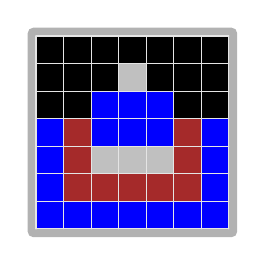
\begin{tikzpicture}
% TikZ grid exported from MARA
\def\cellsz{0.35cm}
\providecommand{\maraGridLineColor}{black!10}
\providecommand{\maraGridBorderColor}{black!30}
\providecommand{\maraGridLineWidth}{0.4pt}
\providecommand{\maraBorderLineWidth}{3pt}
\providecommand{\maraBorderRadius}{2pt}
\begin{scope}[x=\cellsz, y=\cellsz, line cap=round, line join=round]
  % Outer frame as a filled ring expanded by border line width with rounded corners
  \path[fill=\maraGridBorderColor, rounded corners=\maraBorderRadius] ([xshift=-\maraBorderLineWidth,yshift=-\maraBorderLineWidth]0,0) rectangle ([xshift=\maraBorderLineWidth,yshift=\maraBorderLineWidth]7,7);
  % Background
  \fill[black] (0,0) rectangle (7,7);
  % Filled cells
  \begin{scope}[fill={rgb,1:red,0.753;green,0.753;blue,0.753}, fill opacity=1.000]
    \fill (3,5) rectangle ++(1,1);
    \fill (2,2) rectangle ++(1,1);
    \fill (3,2) rectangle ++(1,1);
    \fill (4,2) rectangle ++(1,1);
  \end{scope}
  \begin{scope}[fill={rgb,1:red,0.000;green,0.000;blue,1.000}, fill opacity=1.000]
    \fill (2,4) rectangle ++(1,1);
    \fill (3,4) rectangle ++(1,1);
    \fill (4,4) rectangle ++(1,1);
    \fill (0,3) rectangle ++(1,1);
    \fill (2,3) rectangle ++(1,1);
    \fill (3,3) rectangle ++(1,1);
    \fill (4,3) rectangle ++(1,1);
    \fill (6,3) rectangle ++(1,1);
    \fill (0,2) rectangle ++(1,1);
    \fill (6,2) rectangle ++(1,1);
    \fill (0,1) rectangle ++(1,1);
    \fill (6,1) rectangle ++(1,1);
    \fill (0,0) rectangle ++(1,1);
    \fill (1,0) rectangle ++(1,1);
    \fill (2,0) rectangle ++(1,1);
    \fill (3,0) rectangle ++(1,1);
    \fill (4,0) rectangle ++(1,1);
    \fill (5,0) rectangle ++(1,1);
    \fill (6,0) rectangle ++(1,1);
  \end{scope}
  \begin{scope}[fill={rgb,1:red,0.647;green,0.165;blue,0.165}, fill opacity=1.000]
    \fill (1,3) rectangle ++(1,1);
    \fill (5,3) rectangle ++(1,1);
    \fill (1,2) rectangle ++(1,1);
    \fill (5,2) rectangle ++(1,1);
    \fill (1,1) rectangle ++(1,1);
    \fill (2,1) rectangle ++(1,1);
    \fill (3,1) rectangle ++(1,1);
    \fill (4,1) rectangle ++(1,1);
    \fill (5,1) rectangle ++(1,1);
  \end{scope}
  % Grid and outline
  % Vertical lines
  \begin{scope}[draw=\maraGridLineColor, line width=\maraGridLineWidth, line cap=round]
    \draw (0,0) -- (0,7);
    \draw (1,0) -- (1,7);
    \draw (2,0) -- (2,7);
    \draw (3,0) -- (3,7);
    \draw (4,0) -- (4,7);
    \draw (5,0) -- (5,7);
    \draw (6,0) -- (6,7);
    \draw (7,0) -- (7,7);
  \end{scope}
  % Horizontal lines
  \begin{scope}[draw=\maraGridLineColor, line width=\maraGridLineWidth, line cap=round]
    \draw (0,0) -- (7,0);
    \draw (0,1) -- (7,1);
    \draw (0,2) -- (7,2);
    \draw (0,3) -- (7,3);
    \draw (0,4) -- (7,4);
    \draw (0,5) -- (7,5);
    \draw (0,6) -- (7,6);
    \draw (0,7) -- (7,7);
  \end{scope}
\end{scope}
\end{tikzpicture}
\ActionSequence{\ActionItem{click(3,1)}}
\medskip
% Step 11: noop x1
\smallskip
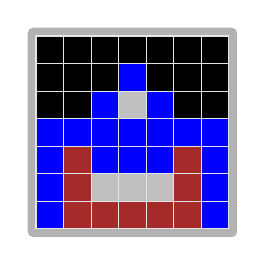
\begin{tikzpicture}
% TikZ grid exported from MARA
\def\cellsz{0.35cm}
\providecommand{\maraGridLineColor}{black!10}
\providecommand{\maraGridBorderColor}{black!30}
\providecommand{\maraGridLineWidth}{0.4pt}
\providecommand{\maraBorderLineWidth}{3pt}
\providecommand{\maraBorderRadius}{2pt}
\begin{scope}[x=\cellsz, y=\cellsz, line cap=round, line join=round]
  % Outer frame as a filled ring expanded by border line width with rounded corners
  \path[fill=\maraGridBorderColor, rounded corners=\maraBorderRadius] ([xshift=-\maraBorderLineWidth,yshift=-\maraBorderLineWidth]0,0) rectangle ([xshift=\maraBorderLineWidth,yshift=\maraBorderLineWidth]7,7);
  % Background
  \fill[black] (0,0) rectangle (7,7);
  % Filled cells
  \begin{scope}[fill={rgb,1:red,0.000;green,0.000;blue,1.000}, fill opacity=1.000]
    \fill (3,5) rectangle ++(1,1);
    \fill (2,4) rectangle ++(1,1);
    \fill (4,4) rectangle ++(1,1);
    \fill (0,3) rectangle ++(1,1);
    \fill (1,3) rectangle ++(1,1);
    \fill (2,3) rectangle ++(1,1);
    \fill (3,3) rectangle ++(1,1);
    \fill (4,3) rectangle ++(1,1);
    \fill (5,3) rectangle ++(1,1);
    \fill (6,3) rectangle ++(1,1);
    \fill (0,2) rectangle ++(1,1);
    \fill (2,2) rectangle ++(1,1);
    \fill (3,2) rectangle ++(1,1);
    \fill (4,2) rectangle ++(1,1);
    \fill (6,2) rectangle ++(1,1);
    \fill (0,1) rectangle ++(1,1);
    \fill (6,1) rectangle ++(1,1);
    \fill (0,0) rectangle ++(1,1);
    \fill (6,0) rectangle ++(1,1);
  \end{scope}
  \begin{scope}[fill={rgb,1:red,0.753;green,0.753;blue,0.753}, fill opacity=1.000]
    \fill (3,4) rectangle ++(1,1);
    \fill (2,1) rectangle ++(1,1);
    \fill (3,1) rectangle ++(1,1);
    \fill (4,1) rectangle ++(1,1);
  \end{scope}
  \begin{scope}[fill={rgb,1:red,0.647;green,0.165;blue,0.165}, fill opacity=1.000]
    \fill (1,2) rectangle ++(1,1);
    \fill (5,2) rectangle ++(1,1);
    \fill (1,1) rectangle ++(1,1);
    \fill (5,1) rectangle ++(1,1);
    \fill (1,0) rectangle ++(1,1);
    \fill (2,0) rectangle ++(1,1);
    \fill (3,0) rectangle ++(1,1);
    \fill (4,0) rectangle ++(1,1);
    \fill (5,0) rectangle ++(1,1);
  \end{scope}
  % Grid and outline
  % Vertical lines
  \begin{scope}[draw=\maraGridLineColor, line width=\maraGridLineWidth, line cap=round]
    \draw (0,0) -- (0,7);
    \draw (1,0) -- (1,7);
    \draw (2,0) -- (2,7);
    \draw (3,0) -- (3,7);
    \draw (4,0) -- (4,7);
    \draw (5,0) -- (5,7);
    \draw (6,0) -- (6,7);
    \draw (7,0) -- (7,7);
  \end{scope}
  % Horizontal lines
  \begin{scope}[draw=\maraGridLineColor, line width=\maraGridLineWidth, line cap=round]
    \draw (0,0) -- (7,0);
    \draw (0,1) -- (7,1);
    \draw (0,2) -- (7,2);
    \draw (0,3) -- (7,3);
    \draw (0,4) -- (7,4);
    \draw (0,5) -- (7,5);
    \draw (0,6) -- (7,6);
    \draw (0,7) -- (7,7);
  \end{scope}
\end{scope}
\end{tikzpicture}
\ActionSequence{\ActionItem{noop x1}}
\medskip
% Step 12: noop x1
\smallskip
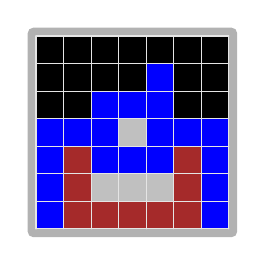
\begin{tikzpicture}
% TikZ grid exported from MARA
\def\cellsz{0.35cm}
\providecommand{\maraGridLineColor}{black!10}
\providecommand{\maraGridBorderColor}{black!30}
\providecommand{\maraGridLineWidth}{0.4pt}
\providecommand{\maraBorderLineWidth}{3pt}
\providecommand{\maraBorderRadius}{2pt}
\begin{scope}[x=\cellsz, y=\cellsz, line cap=round, line join=round]
  % Outer frame as a filled ring expanded by border line width with rounded corners
  \path[fill=\maraGridBorderColor, rounded corners=\maraBorderRadius] ([xshift=-\maraBorderLineWidth,yshift=-\maraBorderLineWidth]0,0) rectangle ([xshift=\maraBorderLineWidth,yshift=\maraBorderLineWidth]7,7);
  % Background
  \fill[black] (0,0) rectangle (7,7);
  % Filled cells
  \begin{scope}[fill={rgb,1:red,0.000;green,0.000;blue,1.000}, fill opacity=1.000]
    \fill (4,5) rectangle ++(1,1);
    \fill (2,4) rectangle ++(1,1);
    \fill (3,4) rectangle ++(1,1);
    \fill (4,4) rectangle ++(1,1);
    \fill (0,3) rectangle ++(1,1);
    \fill (1,3) rectangle ++(1,1);
    \fill (2,3) rectangle ++(1,1);
    \fill (4,3) rectangle ++(1,1);
    \fill (5,3) rectangle ++(1,1);
    \fill (6,3) rectangle ++(1,1);
    \fill (0,2) rectangle ++(1,1);
    \fill (2,2) rectangle ++(1,1);
    \fill (3,2) rectangle ++(1,1);
    \fill (4,2) rectangle ++(1,1);
    \fill (6,2) rectangle ++(1,1);
    \fill (0,1) rectangle ++(1,1);
    \fill (6,1) rectangle ++(1,1);
    \fill (0,0) rectangle ++(1,1);
    \fill (6,0) rectangle ++(1,1);
  \end{scope}
  \begin{scope}[fill={rgb,1:red,0.753;green,0.753;blue,0.753}, fill opacity=1.000]
    \fill (3,3) rectangle ++(1,1);
    \fill (2,1) rectangle ++(1,1);
    \fill (3,1) rectangle ++(1,1);
    \fill (4,1) rectangle ++(1,1);
  \end{scope}
  \begin{scope}[fill={rgb,1:red,0.647;green,0.165;blue,0.165}, fill opacity=1.000]
    \fill (1,2) rectangle ++(1,1);
    \fill (5,2) rectangle ++(1,1);
    \fill (1,1) rectangle ++(1,1);
    \fill (5,1) rectangle ++(1,1);
    \fill (1,0) rectangle ++(1,1);
    \fill (2,0) rectangle ++(1,1);
    \fill (3,0) rectangle ++(1,1);
    \fill (4,0) rectangle ++(1,1);
    \fill (5,0) rectangle ++(1,1);
  \end{scope}
  % Grid and outline
  % Vertical lines
  \begin{scope}[draw=\maraGridLineColor, line width=\maraGridLineWidth, line cap=round]
    \draw (0,0) -- (0,7);
    \draw (1,0) -- (1,7);
    \draw (2,0) -- (2,7);
    \draw (3,0) -- (3,7);
    \draw (4,0) -- (4,7);
    \draw (5,0) -- (5,7);
    \draw (6,0) -- (6,7);
    \draw (7,0) -- (7,7);
  \end{scope}
  % Horizontal lines
  \begin{scope}[draw=\maraGridLineColor, line width=\maraGridLineWidth, line cap=round]
    \draw (0,0) -- (7,0);
    \draw (0,1) -- (7,1);
    \draw (0,2) -- (7,2);
    \draw (0,3) -- (7,3);
    \draw (0,4) -- (7,4);
    \draw (0,5) -- (7,5);
    \draw (0,6) -- (7,6);
    \draw (0,7) -- (7,7);
  \end{scope}
\end{scope}
\end{tikzpicture}
\ActionSequence{\ActionItem{noop x1}}
\medskip
% Step 13: noop x1
\smallskip
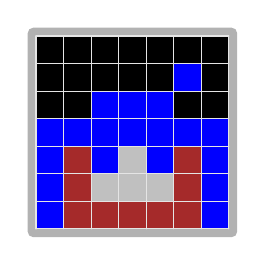
\begin{tikzpicture}
% TikZ grid exported from MARA
\def\cellsz{0.35cm}
\providecommand{\maraGridLineColor}{black!10}
\providecommand{\maraGridBorderColor}{black!30}
\providecommand{\maraGridLineWidth}{0.4pt}
\providecommand{\maraBorderLineWidth}{3pt}
\providecommand{\maraBorderRadius}{2pt}
\begin{scope}[x=\cellsz, y=\cellsz, line cap=round, line join=round]
  % Outer frame as a filled ring expanded by border line width with rounded corners
  \path[fill=\maraGridBorderColor, rounded corners=\maraBorderRadius] ([xshift=-\maraBorderLineWidth,yshift=-\maraBorderLineWidth]0,0) rectangle ([xshift=\maraBorderLineWidth,yshift=\maraBorderLineWidth]7,7);
  % Background
  \fill[black] (0,0) rectangle (7,7);
  % Filled cells
  \begin{scope}[fill={rgb,1:red,0.000;green,0.000;blue,1.000}, fill opacity=1.000]
    \fill (5,5) rectangle ++(1,1);
    \fill (2,4) rectangle ++(1,1);
    \fill (3,4) rectangle ++(1,1);
    \fill (4,4) rectangle ++(1,1);
    \fill (0,3) rectangle ++(1,1);
    \fill (1,3) rectangle ++(1,1);
    \fill (2,3) rectangle ++(1,1);
    \fill (3,3) rectangle ++(1,1);
    \fill (4,3) rectangle ++(1,1);
    \fill (5,3) rectangle ++(1,1);
    \fill (6,3) rectangle ++(1,1);
    \fill (0,2) rectangle ++(1,1);
    \fill (2,2) rectangle ++(1,1);
    \fill (4,2) rectangle ++(1,1);
    \fill (6,2) rectangle ++(1,1);
    \fill (0,1) rectangle ++(1,1);
    \fill (6,1) rectangle ++(1,1);
    \fill (0,0) rectangle ++(1,1);
    \fill (6,0) rectangle ++(1,1);
  \end{scope}
  \begin{scope}[fill={rgb,1:red,0.647;green,0.165;blue,0.165}, fill opacity=1.000]
    \fill (1,2) rectangle ++(1,1);
    \fill (5,2) rectangle ++(1,1);
    \fill (1,1) rectangle ++(1,1);
    \fill (5,1) rectangle ++(1,1);
    \fill (1,0) rectangle ++(1,1);
    \fill (2,0) rectangle ++(1,1);
    \fill (3,0) rectangle ++(1,1);
    \fill (4,0) rectangle ++(1,1);
    \fill (5,0) rectangle ++(1,1);
  \end{scope}
  \begin{scope}[fill={rgb,1:red,0.753;green,0.753;blue,0.753}, fill opacity=1.000]
    \fill (3,2) rectangle ++(1,1);
    \fill (2,1) rectangle ++(1,1);
    \fill (3,1) rectangle ++(1,1);
    \fill (4,1) rectangle ++(1,1);
  \end{scope}
  % Grid and outline
  % Vertical lines
  \begin{scope}[draw=\maraGridLineColor, line width=\maraGridLineWidth, line cap=round]
    \draw (0,0) -- (0,7);
    \draw (1,0) -- (1,7);
    \draw (2,0) -- (2,7);
    \draw (3,0) -- (3,7);
    \draw (4,0) -- (4,7);
    \draw (5,0) -- (5,7);
    \draw (6,0) -- (6,7);
    \draw (7,0) -- (7,7);
  \end{scope}
  % Horizontal lines
  \begin{scope}[draw=\maraGridLineColor, line width=\maraGridLineWidth, line cap=round]
    \draw (0,0) -- (7,0);
    \draw (0,1) -- (7,1);
    \draw (0,2) -- (7,2);
    \draw (0,3) -- (7,3);
    \draw (0,4) -- (7,4);
    \draw (0,5) -- (7,5);
    \draw (0,6) -- (7,6);
    \draw (0,7) -- (7,7);
  \end{scope}
\end{scope}
\end{tikzpicture}
\ActionSequence{\ActionItem{noop x1}}
\medskip
% Step 14: noop x10
\smallskip
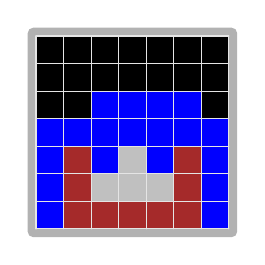
\begin{tikzpicture}
% TikZ grid exported from MARA
\def\cellsz{0.35cm}
\providecommand{\maraGridLineColor}{black!10}
\providecommand{\maraGridBorderColor}{black!30}
\providecommand{\maraGridLineWidth}{0.4pt}
\providecommand{\maraBorderLineWidth}{3pt}
\providecommand{\maraBorderRadius}{2pt}
\begin{scope}[x=\cellsz, y=\cellsz, line cap=round, line join=round]
  % Outer frame as a filled ring expanded by border line width with rounded corners
  \path[fill=\maraGridBorderColor, rounded corners=\maraBorderRadius] ([xshift=-\maraBorderLineWidth,yshift=-\maraBorderLineWidth]0,0) rectangle ([xshift=\maraBorderLineWidth,yshift=\maraBorderLineWidth]7,7);
  % Background
  \fill[black] (0,0) rectangle (7,7);
  % Filled cells
  \begin{scope}[fill={rgb,1:red,0.000;green,0.000;blue,1.000}, fill opacity=1.000]
    \fill (2,4) rectangle ++(1,1);
    \fill (3,4) rectangle ++(1,1);
    \fill (4,4) rectangle ++(1,1);
    \fill (5,4) rectangle ++(1,1);
    \fill (0,3) rectangle ++(1,1);
    \fill (1,3) rectangle ++(1,1);
    \fill (2,3) rectangle ++(1,1);
    \fill (3,3) rectangle ++(1,1);
    \fill (4,3) rectangle ++(1,1);
    \fill (5,3) rectangle ++(1,1);
    \fill (6,3) rectangle ++(1,1);
    \fill (0,2) rectangle ++(1,1);
    \fill (2,2) rectangle ++(1,1);
    \fill (4,2) rectangle ++(1,1);
    \fill (6,2) rectangle ++(1,1);
    \fill (0,1) rectangle ++(1,1);
    \fill (6,1) rectangle ++(1,1);
    \fill (0,0) rectangle ++(1,1);
    \fill (6,0) rectangle ++(1,1);
  \end{scope}
  \begin{scope}[fill={rgb,1:red,0.647;green,0.165;blue,0.165}, fill opacity=1.000]
    \fill (1,2) rectangle ++(1,1);
    \fill (5,2) rectangle ++(1,1);
    \fill (1,1) rectangle ++(1,1);
    \fill (5,1) rectangle ++(1,1);
    \fill (1,0) rectangle ++(1,1);
    \fill (2,0) rectangle ++(1,1);
    \fill (3,0) rectangle ++(1,1);
    \fill (4,0) rectangle ++(1,1);
    \fill (5,0) rectangle ++(1,1);
  \end{scope}
  \begin{scope}[fill={rgb,1:red,0.753;green,0.753;blue,0.753}, fill opacity=1.000]
    \fill (3,2) rectangle ++(1,1);
    \fill (2,1) rectangle ++(1,1);
    \fill (3,1) rectangle ++(1,1);
    \fill (4,1) rectangle ++(1,1);
  \end{scope}
  % Grid and outline
  % Vertical lines
  \begin{scope}[draw=\maraGridLineColor, line width=\maraGridLineWidth, line cap=round]
    \draw (0,0) -- (0,7);
    \draw (1,0) -- (1,7);
    \draw (2,0) -- (2,7);
    \draw (3,0) -- (3,7);
    \draw (4,0) -- (4,7);
    \draw (5,0) -- (5,7);
    \draw (6,0) -- (6,7);
    \draw (7,0) -- (7,7);
  \end{scope}
  % Horizontal lines
  \begin{scope}[draw=\maraGridLineColor, line width=\maraGridLineWidth, line cap=round]
    \draw (0,0) -- (7,0);
    \draw (0,1) -- (7,1);
    \draw (0,2) -- (7,2);
    \draw (0,3) -- (7,3);
    \draw (0,4) -- (7,4);
    \draw (0,5) -- (7,5);
    \draw (0,6) -- (7,6);
    \draw (0,7) -- (7,7);
  \end{scope}
\end{scope}
\end{tikzpicture}
\ActionSequence{\ActionItem{noop x10}}
\medskip
% Step 15: click(1,2)
\smallskip
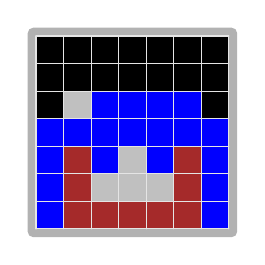
\begin{tikzpicture}
% TikZ grid exported from MARA
\def\cellsz{0.35cm}
\providecommand{\maraGridLineColor}{black!10}
\providecommand{\maraGridBorderColor}{black!30}
\providecommand{\maraGridLineWidth}{0.4pt}
\providecommand{\maraBorderLineWidth}{3pt}
\providecommand{\maraBorderRadius}{2pt}
\begin{scope}[x=\cellsz, y=\cellsz, line cap=round, line join=round]
  % Outer frame as a filled ring expanded by border line width with rounded corners
  \path[fill=\maraGridBorderColor, rounded corners=\maraBorderRadius] ([xshift=-\maraBorderLineWidth,yshift=-\maraBorderLineWidth]0,0) rectangle ([xshift=\maraBorderLineWidth,yshift=\maraBorderLineWidth]7,7);
  % Background
  \fill[black] (0,0) rectangle (7,7);
  % Filled cells
  \begin{scope}[fill={rgb,1:red,0.753;green,0.753;blue,0.753}, fill opacity=1.000]
    \fill (1,4) rectangle ++(1,1);
    \fill (3,2) rectangle ++(1,1);
    \fill (2,1) rectangle ++(1,1);
    \fill (3,1) rectangle ++(1,1);
    \fill (4,1) rectangle ++(1,1);
  \end{scope}
  \begin{scope}[fill={rgb,1:red,0.000;green,0.000;blue,1.000}, fill opacity=1.000]
    \fill (2,4) rectangle ++(1,1);
    \fill (3,4) rectangle ++(1,1);
    \fill (4,4) rectangle ++(1,1);
    \fill (5,4) rectangle ++(1,1);
    \fill (0,3) rectangle ++(1,1);
    \fill (1,3) rectangle ++(1,1);
    \fill (2,3) rectangle ++(1,1);
    \fill (3,3) rectangle ++(1,1);
    \fill (4,3) rectangle ++(1,1);
    \fill (5,3) rectangle ++(1,1);
    \fill (6,3) rectangle ++(1,1);
    \fill (0,2) rectangle ++(1,1);
    \fill (2,2) rectangle ++(1,1);
    \fill (4,2) rectangle ++(1,1);
    \fill (6,2) rectangle ++(1,1);
    \fill (0,1) rectangle ++(1,1);
    \fill (6,1) rectangle ++(1,1);
    \fill (0,0) rectangle ++(1,1);
    \fill (6,0) rectangle ++(1,1);
  \end{scope}
  \begin{scope}[fill={rgb,1:red,0.647;green,0.165;blue,0.165}, fill opacity=1.000]
    \fill (1,2) rectangle ++(1,1);
    \fill (5,2) rectangle ++(1,1);
    \fill (1,1) rectangle ++(1,1);
    \fill (5,1) rectangle ++(1,1);
    \fill (1,0) rectangle ++(1,1);
    \fill (2,0) rectangle ++(1,1);
    \fill (3,0) rectangle ++(1,1);
    \fill (4,0) rectangle ++(1,1);
    \fill (5,0) rectangle ++(1,1);
  \end{scope}
  % Grid and outline
  % Vertical lines
  \begin{scope}[draw=\maraGridLineColor, line width=\maraGridLineWidth, line cap=round]
    \draw (0,0) -- (0,7);
    \draw (1,0) -- (1,7);
    \draw (2,0) -- (2,7);
    \draw (3,0) -- (3,7);
    \draw (4,0) -- (4,7);
    \draw (5,0) -- (5,7);
    \draw (6,0) -- (6,7);
    \draw (7,0) -- (7,7);
  \end{scope}
  % Horizontal lines
  \begin{scope}[draw=\maraGridLineColor, line width=\maraGridLineWidth, line cap=round]
    \draw (0,0) -- (7,0);
    \draw (0,1) -- (7,1);
    \draw (0,2) -- (7,2);
    \draw (0,3) -- (7,3);
    \draw (0,4) -- (7,4);
    \draw (0,5) -- (7,5);
    \draw (0,6) -- (7,6);
    \draw (0,7) -- (7,7);
  \end{scope}
\end{scope}
\end{tikzpicture}
\ActionSequence{\ActionItem{click(1,2)}}
\medskip
% Step 16: noop x4
\smallskip
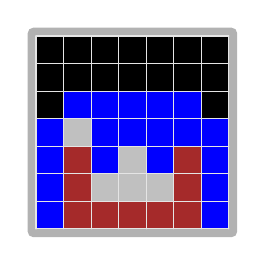
\begin{tikzpicture}
% TikZ grid exported from MARA
\def\cellsz{0.35cm}
\providecommand{\maraGridLineColor}{black!10}
\providecommand{\maraGridBorderColor}{black!30}
\providecommand{\maraGridLineWidth}{0.4pt}
\providecommand{\maraBorderLineWidth}{3pt}
\providecommand{\maraBorderRadius}{2pt}
\begin{scope}[x=\cellsz, y=\cellsz, line cap=round, line join=round]
  % Outer frame as a filled ring expanded by border line width with rounded corners
  \path[fill=\maraGridBorderColor, rounded corners=\maraBorderRadius] ([xshift=-\maraBorderLineWidth,yshift=-\maraBorderLineWidth]0,0) rectangle ([xshift=\maraBorderLineWidth,yshift=\maraBorderLineWidth]7,7);
  % Background
  \fill[black] (0,0) rectangle (7,7);
  % Filled cells
  \begin{scope}[fill={rgb,1:red,0.000;green,0.000;blue,1.000}, fill opacity=1.000]
    \fill (1,4) rectangle ++(1,1);
    \fill (2,4) rectangle ++(1,1);
    \fill (3,4) rectangle ++(1,1);
    \fill (4,4) rectangle ++(1,1);
    \fill (5,4) rectangle ++(1,1);
    \fill (0,3) rectangle ++(1,1);
    \fill (2,3) rectangle ++(1,1);
    \fill (3,3) rectangle ++(1,1);
    \fill (4,3) rectangle ++(1,1);
    \fill (5,3) rectangle ++(1,1);
    \fill (6,3) rectangle ++(1,1);
    \fill (0,2) rectangle ++(1,1);
    \fill (2,2) rectangle ++(1,1);
    \fill (4,2) rectangle ++(1,1);
    \fill (6,2) rectangle ++(1,1);
    \fill (0,1) rectangle ++(1,1);
    \fill (6,1) rectangle ++(1,1);
    \fill (0,0) rectangle ++(1,1);
    \fill (6,0) rectangle ++(1,1);
  \end{scope}
  \begin{scope}[fill={rgb,1:red,0.753;green,0.753;blue,0.753}, fill opacity=1.000]
    \fill (1,3) rectangle ++(1,1);
    \fill (3,2) rectangle ++(1,1);
    \fill (2,1) rectangle ++(1,1);
    \fill (3,1) rectangle ++(1,1);
    \fill (4,1) rectangle ++(1,1);
  \end{scope}
  \begin{scope}[fill={rgb,1:red,0.647;green,0.165;blue,0.165}, fill opacity=1.000]
    \fill (1,2) rectangle ++(1,1);
    \fill (5,2) rectangle ++(1,1);
    \fill (1,1) rectangle ++(1,1);
    \fill (5,1) rectangle ++(1,1);
    \fill (1,0) rectangle ++(1,1);
    \fill (2,0) rectangle ++(1,1);
    \fill (3,0) rectangle ++(1,1);
    \fill (4,0) rectangle ++(1,1);
    \fill (5,0) rectangle ++(1,1);
  \end{scope}
  % Grid and outline
  % Vertical lines
  \begin{scope}[draw=\maraGridLineColor, line width=\maraGridLineWidth, line cap=round]
    \draw (0,0) -- (0,7);
    \draw (1,0) -- (1,7);
    \draw (2,0) -- (2,7);
    \draw (3,0) -- (3,7);
    \draw (4,0) -- (4,7);
    \draw (5,0) -- (5,7);
    \draw (6,0) -- (6,7);
    \draw (7,0) -- (7,7);
  \end{scope}
  % Horizontal lines
  \begin{scope}[draw=\maraGridLineColor, line width=\maraGridLineWidth, line cap=round]
    \draw (0,0) -- (7,0);
    \draw (0,1) -- (7,1);
    \draw (0,2) -- (7,2);
    \draw (0,3) -- (7,3);
    \draw (0,4) -- (7,4);
    \draw (0,5) -- (7,5);
    \draw (0,6) -- (7,6);
    \draw (0,7) -- (7,7);
  \end{scope}
\end{scope}
\end{tikzpicture}
\ActionSequence{\ActionItem{noop x4}}
\medskip
% Step 17: click(0,2)
\smallskip
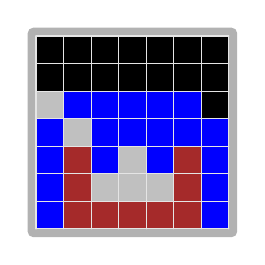
\begin{tikzpicture}
% TikZ grid exported from MARA
\def\cellsz{0.35cm}
\providecommand{\maraGridLineColor}{black!10}
\providecommand{\maraGridBorderColor}{black!30}
\providecommand{\maraGridLineWidth}{0.4pt}
\providecommand{\maraBorderLineWidth}{3pt}
\providecommand{\maraBorderRadius}{2pt}
\begin{scope}[x=\cellsz, y=\cellsz, line cap=round, line join=round]
  % Outer frame as a filled ring expanded by border line width with rounded corners
  \path[fill=\maraGridBorderColor, rounded corners=\maraBorderRadius] ([xshift=-\maraBorderLineWidth,yshift=-\maraBorderLineWidth]0,0) rectangle ([xshift=\maraBorderLineWidth,yshift=\maraBorderLineWidth]7,7);
  % Background
  \fill[black] (0,0) rectangle (7,7);
  % Filled cells
  \begin{scope}[fill={rgb,1:red,0.753;green,0.753;blue,0.753}, fill opacity=1.000]
    \fill (0,4) rectangle ++(1,1);
    \fill (1,3) rectangle ++(1,1);
    \fill (3,2) rectangle ++(1,1);
    \fill (2,1) rectangle ++(1,1);
    \fill (3,1) rectangle ++(1,1);
    \fill (4,1) rectangle ++(1,1);
  \end{scope}
  \begin{scope}[fill={rgb,1:red,0.000;green,0.000;blue,1.000}, fill opacity=1.000]
    \fill (1,4) rectangle ++(1,1);
    \fill (2,4) rectangle ++(1,1);
    \fill (3,4) rectangle ++(1,1);
    \fill (4,4) rectangle ++(1,1);
    \fill (5,4) rectangle ++(1,1);
    \fill (0,3) rectangle ++(1,1);
    \fill (2,3) rectangle ++(1,1);
    \fill (3,3) rectangle ++(1,1);
    \fill (4,3) rectangle ++(1,1);
    \fill (5,3) rectangle ++(1,1);
    \fill (6,3) rectangle ++(1,1);
    \fill (0,2) rectangle ++(1,1);
    \fill (2,2) rectangle ++(1,1);
    \fill (4,2) rectangle ++(1,1);
    \fill (6,2) rectangle ++(1,1);
    \fill (0,1) rectangle ++(1,1);
    \fill (6,1) rectangle ++(1,1);
    \fill (0,0) rectangle ++(1,1);
    \fill (6,0) rectangle ++(1,1);
  \end{scope}
  \begin{scope}[fill={rgb,1:red,0.647;green,0.165;blue,0.165}, fill opacity=1.000]
    \fill (1,2) rectangle ++(1,1);
    \fill (5,2) rectangle ++(1,1);
    \fill (1,1) rectangle ++(1,1);
    \fill (5,1) rectangle ++(1,1);
    \fill (1,0) rectangle ++(1,1);
    \fill (2,0) rectangle ++(1,1);
    \fill (3,0) rectangle ++(1,1);
    \fill (4,0) rectangle ++(1,1);
    \fill (5,0) rectangle ++(1,1);
  \end{scope}
  % Grid and outline
  % Vertical lines
  \begin{scope}[draw=\maraGridLineColor, line width=\maraGridLineWidth, line cap=round]
    \draw (0,0) -- (0,7);
    \draw (1,0) -- (1,7);
    \draw (2,0) -- (2,7);
    \draw (3,0) -- (3,7);
    \draw (4,0) -- (4,7);
    \draw (5,0) -- (5,7);
    \draw (6,0) -- (6,7);
    \draw (7,0) -- (7,7);
  \end{scope}
  % Horizontal lines
  \begin{scope}[draw=\maraGridLineColor, line width=\maraGridLineWidth, line cap=round]
    \draw (0,0) -- (7,0);
    \draw (0,1) -- (7,1);
    \draw (0,2) -- (7,2);
    \draw (0,3) -- (7,3);
    \draw (0,4) -- (7,4);
    \draw (0,5) -- (7,5);
    \draw (0,6) -- (7,6);
    \draw (0,7) -- (7,7);
  \end{scope}
\end{scope}
\end{tikzpicture}
\ActionSequence{\ActionItem{click(0,2)}}
\medskip
% Step 18: noop x1
\smallskip
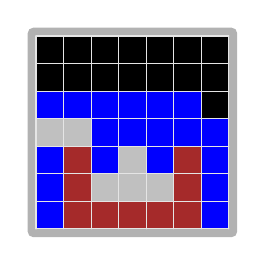
\begin{tikzpicture}
% TikZ grid exported from MARA
\def\cellsz{0.35cm}
\providecommand{\maraGridLineColor}{black!10}
\providecommand{\maraGridBorderColor}{black!30}
\providecommand{\maraGridLineWidth}{0.4pt}
\providecommand{\maraBorderLineWidth}{3pt}
\providecommand{\maraBorderRadius}{2pt}
\begin{scope}[x=\cellsz, y=\cellsz, line cap=round, line join=round]
  % Outer frame as a filled ring expanded by border line width with rounded corners
  \path[fill=\maraGridBorderColor, rounded corners=\maraBorderRadius] ([xshift=-\maraBorderLineWidth,yshift=-\maraBorderLineWidth]0,0) rectangle ([xshift=\maraBorderLineWidth,yshift=\maraBorderLineWidth]7,7);
  % Background
  \fill[black] (0,0) rectangle (7,7);
  % Filled cells
  \begin{scope}[fill={rgb,1:red,0.000;green,0.000;blue,1.000}, fill opacity=1.000]
    \fill (0,4) rectangle ++(1,1);
    \fill (1,4) rectangle ++(1,1);
    \fill (2,4) rectangle ++(1,1);
    \fill (3,4) rectangle ++(1,1);
    \fill (4,4) rectangle ++(1,1);
    \fill (5,4) rectangle ++(1,1);
    \fill (2,3) rectangle ++(1,1);
    \fill (3,3) rectangle ++(1,1);
    \fill (4,3) rectangle ++(1,1);
    \fill (5,3) rectangle ++(1,1);
    \fill (6,3) rectangle ++(1,1);
    \fill (0,2) rectangle ++(1,1);
    \fill (2,2) rectangle ++(1,1);
    \fill (4,2) rectangle ++(1,1);
    \fill (6,2) rectangle ++(1,1);
    \fill (0,1) rectangle ++(1,1);
    \fill (6,1) rectangle ++(1,1);
    \fill (0,0) rectangle ++(1,1);
    \fill (6,0) rectangle ++(1,1);
  \end{scope}
  \begin{scope}[fill={rgb,1:red,0.753;green,0.753;blue,0.753}, fill opacity=1.000]
    \fill (0,3) rectangle ++(1,1);
    \fill (1,3) rectangle ++(1,1);
    \fill (3,2) rectangle ++(1,1);
    \fill (2,1) rectangle ++(1,1);
    \fill (3,1) rectangle ++(1,1);
    \fill (4,1) rectangle ++(1,1);
  \end{scope}
  \begin{scope}[fill={rgb,1:red,0.647;green,0.165;blue,0.165}, fill opacity=1.000]
    \fill (1,2) rectangle ++(1,1);
    \fill (5,2) rectangle ++(1,1);
    \fill (1,1) rectangle ++(1,1);
    \fill (5,1) rectangle ++(1,1);
    \fill (1,0) rectangle ++(1,1);
    \fill (2,0) rectangle ++(1,1);
    \fill (3,0) rectangle ++(1,1);
    \fill (4,0) rectangle ++(1,1);
    \fill (5,0) rectangle ++(1,1);
  \end{scope}
  % Grid and outline
  % Vertical lines
  \begin{scope}[draw=\maraGridLineColor, line width=\maraGridLineWidth, line cap=round]
    \draw (0,0) -- (0,7);
    \draw (1,0) -- (1,7);
    \draw (2,0) -- (2,7);
    \draw (3,0) -- (3,7);
    \draw (4,0) -- (4,7);
    \draw (5,0) -- (5,7);
    \draw (6,0) -- (6,7);
    \draw (7,0) -- (7,7);
  \end{scope}
  % Horizontal lines
  \begin{scope}[draw=\maraGridLineColor, line width=\maraGridLineWidth, line cap=round]
    \draw (0,0) -- (7,0);
    \draw (0,1) -- (7,1);
    \draw (0,2) -- (7,2);
    \draw (0,3) -- (7,3);
    \draw (0,4) -- (7,4);
    \draw (0,5) -- (7,5);
    \draw (0,6) -- (7,6);
    \draw (0,7) -- (7,7);
  \end{scope}
\end{scope}
\end{tikzpicture}
\ActionSequence{\ActionItem{noop x1}}
\medskip
% Step 19: noop x1
\smallskip
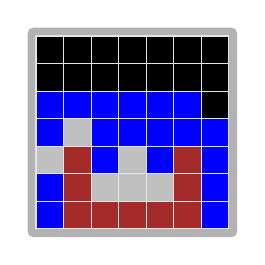
\begin{tikzpicture}
% TikZ grid exported from MARA
\def\cellsz{0.35cm}
\providecommand{\maraGridLineColor}{black!10}
\providecommand{\maraGridBorderColor}{black!30}
\providecommand{\maraGridLineWidth}{0.4pt}
\providecommand{\maraBorderLineWidth}{3pt}
\providecommand{\maraBorderRadius}{2pt}
\begin{scope}[x=\cellsz, y=\cellsz, line cap=round, line join=round]
  % Outer frame as a filled ring expanded by border line width with rounded corners
  \path[fill=\maraGridBorderColor, rounded corners=\maraBorderRadius] ([xshift=-\maraBorderLineWidth,yshift=-\maraBorderLineWidth]0,0) rectangle ([xshift=\maraBorderLineWidth,yshift=\maraBorderLineWidth]7,7);
  % Background
  \fill[black] (0,0) rectangle (7,7);
  % Filled cells
  \begin{scope}[fill={rgb,1:red,0.000;green,0.000;blue,1.000}, fill opacity=1.000]
    \fill (0,4) rectangle ++(1,1);
    \fill (1,4) rectangle ++(1,1);
    \fill (2,4) rectangle ++(1,1);
    \fill (3,4) rectangle ++(1,1);
    \fill (4,4) rectangle ++(1,1);
    \fill (5,4) rectangle ++(1,1);
    \fill (0,3) rectangle ++(1,1);
    \fill (2,3) rectangle ++(1,1);
    \fill (3,3) rectangle ++(1,1);
    \fill (4,3) rectangle ++(1,1);
    \fill (5,3) rectangle ++(1,1);
    \fill (6,3) rectangle ++(1,1);
    \fill (2,2) rectangle ++(1,1);
    \fill (4,2) rectangle ++(1,1);
    \fill (6,2) rectangle ++(1,1);
    \fill (0,1) rectangle ++(1,1);
    \fill (6,1) rectangle ++(1,1);
    \fill (0,0) rectangle ++(1,1);
    \fill (6,0) rectangle ++(1,1);
  \end{scope}
  \begin{scope}[fill={rgb,1:red,0.753;green,0.753;blue,0.753}, fill opacity=1.000]
    \fill (1,3) rectangle ++(1,1);
    \fill (0,2) rectangle ++(1,1);
    \fill (3,2) rectangle ++(1,1);
    \fill (2,1) rectangle ++(1,1);
    \fill (3,1) rectangle ++(1,1);
    \fill (4,1) rectangle ++(1,1);
  \end{scope}
  \begin{scope}[fill={rgb,1:red,0.647;green,0.165;blue,0.165}, fill opacity=1.000]
    \fill (1,2) rectangle ++(1,1);
    \fill (5,2) rectangle ++(1,1);
    \fill (1,1) rectangle ++(1,1);
    \fill (5,1) rectangle ++(1,1);
    \fill (1,0) rectangle ++(1,1);
    \fill (2,0) rectangle ++(1,1);
    \fill (3,0) rectangle ++(1,1);
    \fill (4,0) rectangle ++(1,1);
    \fill (5,0) rectangle ++(1,1);
  \end{scope}
  % Grid and outline
  % Vertical lines
  \begin{scope}[draw=\maraGridLineColor, line width=\maraGridLineWidth, line cap=round]
    \draw (0,0) -- (0,7);
    \draw (1,0) -- (1,7);
    \draw (2,0) -- (2,7);
    \draw (3,0) -- (3,7);
    \draw (4,0) -- (4,7);
    \draw (5,0) -- (5,7);
    \draw (6,0) -- (6,7);
    \draw (7,0) -- (7,7);
  \end{scope}
  % Horizontal lines
  \begin{scope}[draw=\maraGridLineColor, line width=\maraGridLineWidth, line cap=round]
    \draw (0,0) -- (7,0);
    \draw (0,1) -- (7,1);
    \draw (0,2) -- (7,2);
    \draw (0,3) -- (7,3);
    \draw (0,4) -- (7,4);
    \draw (0,5) -- (7,5);
    \draw (0,6) -- (7,6);
    \draw (0,7) -- (7,7);
  \end{scope}
\end{scope}
\end{tikzpicture}
\ActionSequence{\ActionItem{noop x1}}
\medskip
% Step 20: noop x1
\smallskip
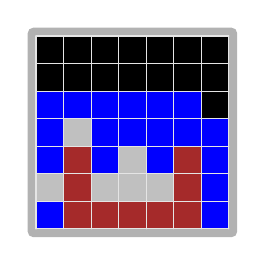
\begin{tikzpicture}
% TikZ grid exported from MARA
\def\cellsz{0.35cm}
\providecommand{\maraGridLineColor}{black!10}
\providecommand{\maraGridBorderColor}{black!30}
\providecommand{\maraGridLineWidth}{0.4pt}
\providecommand{\maraBorderLineWidth}{3pt}
\providecommand{\maraBorderRadius}{2pt}
\begin{scope}[x=\cellsz, y=\cellsz, line cap=round, line join=round]
  % Outer frame as a filled ring expanded by border line width with rounded corners
  \path[fill=\maraGridBorderColor, rounded corners=\maraBorderRadius] ([xshift=-\maraBorderLineWidth,yshift=-\maraBorderLineWidth]0,0) rectangle ([xshift=\maraBorderLineWidth,yshift=\maraBorderLineWidth]7,7);
  % Background
  \fill[black] (0,0) rectangle (7,7);
  % Filled cells
  \begin{scope}[fill={rgb,1:red,0.000;green,0.000;blue,1.000}, fill opacity=1.000]
    \fill (0,4) rectangle ++(1,1);
    \fill (1,4) rectangle ++(1,1);
    \fill (2,4) rectangle ++(1,1);
    \fill (3,4) rectangle ++(1,1);
    \fill (4,4) rectangle ++(1,1);
    \fill (5,4) rectangle ++(1,1);
    \fill (0,3) rectangle ++(1,1);
    \fill (2,3) rectangle ++(1,1);
    \fill (3,3) rectangle ++(1,1);
    \fill (4,3) rectangle ++(1,1);
    \fill (5,3) rectangle ++(1,1);
    \fill (6,3) rectangle ++(1,1);
    \fill (0,2) rectangle ++(1,1);
    \fill (2,2) rectangle ++(1,1);
    \fill (4,2) rectangle ++(1,1);
    \fill (6,2) rectangle ++(1,1);
    \fill (6,1) rectangle ++(1,1);
    \fill (0,0) rectangle ++(1,1);
    \fill (6,0) rectangle ++(1,1);
  \end{scope}
  \begin{scope}[fill={rgb,1:red,0.753;green,0.753;blue,0.753}, fill opacity=1.000]
    \fill (1,3) rectangle ++(1,1);
    \fill (3,2) rectangle ++(1,1);
    \fill (0,1) rectangle ++(1,1);
    \fill (2,1) rectangle ++(1,1);
    \fill (3,1) rectangle ++(1,1);
    \fill (4,1) rectangle ++(1,1);
  \end{scope}
  \begin{scope}[fill={rgb,1:red,0.647;green,0.165;blue,0.165}, fill opacity=1.000]
    \fill (1,2) rectangle ++(1,1);
    \fill (5,2) rectangle ++(1,1);
    \fill (1,1) rectangle ++(1,1);
    \fill (5,1) rectangle ++(1,1);
    \fill (1,0) rectangle ++(1,1);
    \fill (2,0) rectangle ++(1,1);
    \fill (3,0) rectangle ++(1,1);
    \fill (4,0) rectangle ++(1,1);
    \fill (5,0) rectangle ++(1,1);
  \end{scope}
  % Grid and outline
  % Vertical lines
  \begin{scope}[draw=\maraGridLineColor, line width=\maraGridLineWidth, line cap=round]
    \draw (0,0) -- (0,7);
    \draw (1,0) -- (1,7);
    \draw (2,0) -- (2,7);
    \draw (3,0) -- (3,7);
    \draw (4,0) -- (4,7);
    \draw (5,0) -- (5,7);
    \draw (6,0) -- (6,7);
    \draw (7,0) -- (7,7);
  \end{scope}
  % Horizontal lines
  \begin{scope}[draw=\maraGridLineColor, line width=\maraGridLineWidth, line cap=round]
    \draw (0,0) -- (7,0);
    \draw (0,1) -- (7,1);
    \draw (0,2) -- (7,2);
    \draw (0,3) -- (7,3);
    \draw (0,4) -- (7,4);
    \draw (0,5) -- (7,5);
    \draw (0,6) -- (7,6);
    \draw (0,7) -- (7,7);
  \end{scope}
\end{scope}
\end{tikzpicture}
\ActionSequence{\ActionItem{noop x1}}
\medskip
% Step 21: click(0,1)
\smallskip
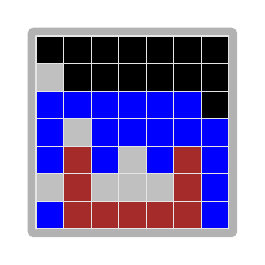
\begin{tikzpicture}
% TikZ grid exported from MARA
\def\cellsz{0.35cm}
\providecommand{\maraGridLineColor}{black!10}
\providecommand{\maraGridBorderColor}{black!30}
\providecommand{\maraGridLineWidth}{0.4pt}
\providecommand{\maraBorderLineWidth}{3pt}
\providecommand{\maraBorderRadius}{2pt}
\begin{scope}[x=\cellsz, y=\cellsz, line cap=round, line join=round]
  % Outer frame as a filled ring expanded by border line width with rounded corners
  \path[fill=\maraGridBorderColor, rounded corners=\maraBorderRadius] ([xshift=-\maraBorderLineWidth,yshift=-\maraBorderLineWidth]0,0) rectangle ([xshift=\maraBorderLineWidth,yshift=\maraBorderLineWidth]7,7);
  % Background
  \fill[black] (0,0) rectangle (7,7);
  % Filled cells
  \begin{scope}[fill={rgb,1:red,0.753;green,0.753;blue,0.753}, fill opacity=1.000]
    \fill (0,5) rectangle ++(1,1);
    \fill (1,3) rectangle ++(1,1);
    \fill (3,2) rectangle ++(1,1);
    \fill (0,1) rectangle ++(1,1);
    \fill (2,1) rectangle ++(1,1);
    \fill (3,1) rectangle ++(1,1);
    \fill (4,1) rectangle ++(1,1);
  \end{scope}
  \begin{scope}[fill={rgb,1:red,0.000;green,0.000;blue,1.000}, fill opacity=1.000]
    \fill (0,4) rectangle ++(1,1);
    \fill (1,4) rectangle ++(1,1);
    \fill (2,4) rectangle ++(1,1);
    \fill (3,4) rectangle ++(1,1);
    \fill (4,4) rectangle ++(1,1);
    \fill (5,4) rectangle ++(1,1);
    \fill (0,3) rectangle ++(1,1);
    \fill (2,3) rectangle ++(1,1);
    \fill (3,3) rectangle ++(1,1);
    \fill (4,3) rectangle ++(1,1);
    \fill (5,3) rectangle ++(1,1);
    \fill (6,3) rectangle ++(1,1);
    \fill (0,2) rectangle ++(1,1);
    \fill (2,2) rectangle ++(1,1);
    \fill (4,2) rectangle ++(1,1);
    \fill (6,2) rectangle ++(1,1);
    \fill (6,1) rectangle ++(1,1);
    \fill (0,0) rectangle ++(1,1);
    \fill (6,0) rectangle ++(1,1);
  \end{scope}
  \begin{scope}[fill={rgb,1:red,0.647;green,0.165;blue,0.165}, fill opacity=1.000]
    \fill (1,2) rectangle ++(1,1);
    \fill (5,2) rectangle ++(1,1);
    \fill (1,1) rectangle ++(1,1);
    \fill (5,1) rectangle ++(1,1);
    \fill (1,0) rectangle ++(1,1);
    \fill (2,0) rectangle ++(1,1);
    \fill (3,0) rectangle ++(1,1);
    \fill (4,0) rectangle ++(1,1);
    \fill (5,0) rectangle ++(1,1);
  \end{scope}
  % Grid and outline
  % Vertical lines
  \begin{scope}[draw=\maraGridLineColor, line width=\maraGridLineWidth, line cap=round]
    \draw (0,0) -- (0,7);
    \draw (1,0) -- (1,7);
    \draw (2,0) -- (2,7);
    \draw (3,0) -- (3,7);
    \draw (4,0) -- (4,7);
    \draw (5,0) -- (5,7);
    \draw (6,0) -- (6,7);
    \draw (7,0) -- (7,7);
  \end{scope}
  % Horizontal lines
  \begin{scope}[draw=\maraGridLineColor, line width=\maraGridLineWidth, line cap=round]
    \draw (0,0) -- (7,0);
    \draw (0,1) -- (7,1);
    \draw (0,2) -- (7,2);
    \draw (0,3) -- (7,3);
    \draw (0,4) -- (7,4);
    \draw (0,5) -- (7,5);
    \draw (0,6) -- (7,6);
    \draw (0,7) -- (7,7);
  \end{scope}
\end{scope}
\end{tikzpicture}
\ActionSequence{\ActionItem{click(0,1)}}
\medskip
% Step 22: noop x1
\smallskip
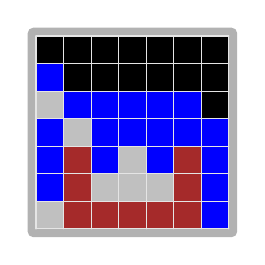
\begin{tikzpicture}
% TikZ grid exported from MARA
\def\cellsz{0.35cm}
\providecommand{\maraGridLineColor}{black!10}
\providecommand{\maraGridBorderColor}{black!30}
\providecommand{\maraGridLineWidth}{0.4pt}
\providecommand{\maraBorderLineWidth}{3pt}
\providecommand{\maraBorderRadius}{2pt}
\begin{scope}[x=\cellsz, y=\cellsz, line cap=round, line join=round]
  % Outer frame as a filled ring expanded by border line width with rounded corners
  \path[fill=\maraGridBorderColor, rounded corners=\maraBorderRadius] ([xshift=-\maraBorderLineWidth,yshift=-\maraBorderLineWidth]0,0) rectangle ([xshift=\maraBorderLineWidth,yshift=\maraBorderLineWidth]7,7);
  % Background
  \fill[black] (0,0) rectangle (7,7);
  % Filled cells
  \begin{scope}[fill={rgb,1:red,0.000;green,0.000;blue,1.000}, fill opacity=1.000]
    \fill (0,5) rectangle ++(1,1);
    \fill (1,4) rectangle ++(1,1);
    \fill (2,4) rectangle ++(1,1);
    \fill (3,4) rectangle ++(1,1);
    \fill (4,4) rectangle ++(1,1);
    \fill (5,4) rectangle ++(1,1);
    \fill (0,3) rectangle ++(1,1);
    \fill (2,3) rectangle ++(1,1);
    \fill (3,3) rectangle ++(1,1);
    \fill (4,3) rectangle ++(1,1);
    \fill (5,3) rectangle ++(1,1);
    \fill (6,3) rectangle ++(1,1);
    \fill (0,2) rectangle ++(1,1);
    \fill (2,2) rectangle ++(1,1);
    \fill (4,2) rectangle ++(1,1);
    \fill (6,2) rectangle ++(1,1);
    \fill (0,1) rectangle ++(1,1);
    \fill (6,1) rectangle ++(1,1);
    \fill (6,0) rectangle ++(1,1);
  \end{scope}
  \begin{scope}[fill={rgb,1:red,0.753;green,0.753;blue,0.753}, fill opacity=1.000]
    \fill (0,4) rectangle ++(1,1);
    \fill (1,3) rectangle ++(1,1);
    \fill (3,2) rectangle ++(1,1);
    \fill (2,1) rectangle ++(1,1);
    \fill (3,1) rectangle ++(1,1);
    \fill (4,1) rectangle ++(1,1);
    \fill (0,0) rectangle ++(1,1);
  \end{scope}
  \begin{scope}[fill={rgb,1:red,0.647;green,0.165;blue,0.165}, fill opacity=1.000]
    \fill (1,2) rectangle ++(1,1);
    \fill (5,2) rectangle ++(1,1);
    \fill (1,1) rectangle ++(1,1);
    \fill (5,1) rectangle ++(1,1);
    \fill (1,0) rectangle ++(1,1);
    \fill (2,0) rectangle ++(1,1);
    \fill (3,0) rectangle ++(1,1);
    \fill (4,0) rectangle ++(1,1);
    \fill (5,0) rectangle ++(1,1);
  \end{scope}
  % Grid and outline
  % Vertical lines
  \begin{scope}[draw=\maraGridLineColor, line width=\maraGridLineWidth, line cap=round]
    \draw (0,0) -- (0,7);
    \draw (1,0) -- (1,7);
    \draw (2,0) -- (2,7);
    \draw (3,0) -- (3,7);
    \draw (4,0) -- (4,7);
    \draw (5,0) -- (5,7);
    \draw (6,0) -- (6,7);
    \draw (7,0) -- (7,7);
  \end{scope}
  % Horizontal lines
  \begin{scope}[draw=\maraGridLineColor, line width=\maraGridLineWidth, line cap=round]
    \draw (0,0) -- (7,0);
    \draw (0,1) -- (7,1);
    \draw (0,2) -- (7,2);
    \draw (0,3) -- (7,3);
    \draw (0,4) -- (7,4);
    \draw (0,5) -- (7,5);
    \draw (0,6) -- (7,6);
    \draw (0,7) -- (7,7);
  \end{scope}
\end{scope}
\end{tikzpicture}
\ActionSequence{\ActionItem{noop x1}}
\medskip
% Step 23: noop x1
\smallskip
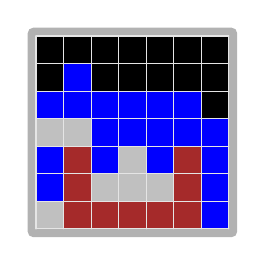
\begin{tikzpicture}
% TikZ grid exported from MARA
\def\cellsz{0.35cm}
\providecommand{\maraGridLineColor}{black!10}
\providecommand{\maraGridBorderColor}{black!30}
\providecommand{\maraGridLineWidth}{0.4pt}
\providecommand{\maraBorderLineWidth}{3pt}
\providecommand{\maraBorderRadius}{2pt}
\begin{scope}[x=\cellsz, y=\cellsz, line cap=round, line join=round]
  % Outer frame as a filled ring expanded by border line width with rounded corners
  \path[fill=\maraGridBorderColor, rounded corners=\maraBorderRadius] ([xshift=-\maraBorderLineWidth,yshift=-\maraBorderLineWidth]0,0) rectangle ([xshift=\maraBorderLineWidth,yshift=\maraBorderLineWidth]7,7);
  % Background
  \fill[black] (0,0) rectangle (7,7);
  % Filled cells
  \begin{scope}[fill={rgb,1:red,0.000;green,0.000;blue,1.000}, fill opacity=1.000]
    \fill (1,5) rectangle ++(1,1);
    \fill (0,4) rectangle ++(1,1);
    \fill (1,4) rectangle ++(1,1);
    \fill (2,4) rectangle ++(1,1);
    \fill (3,4) rectangle ++(1,1);
    \fill (4,4) rectangle ++(1,1);
    \fill (5,4) rectangle ++(1,1);
    \fill (2,3) rectangle ++(1,1);
    \fill (3,3) rectangle ++(1,1);
    \fill (4,3) rectangle ++(1,1);
    \fill (5,3) rectangle ++(1,1);
    \fill (6,3) rectangle ++(1,1);
    \fill (0,2) rectangle ++(1,1);
    \fill (2,2) rectangle ++(1,1);
    \fill (4,2) rectangle ++(1,1);
    \fill (6,2) rectangle ++(1,1);
    \fill (0,1) rectangle ++(1,1);
    \fill (6,1) rectangle ++(1,1);
    \fill (6,0) rectangle ++(1,1);
  \end{scope}
  \begin{scope}[fill={rgb,1:red,0.753;green,0.753;blue,0.753}, fill opacity=1.000]
    \fill (0,3) rectangle ++(1,1);
    \fill (1,3) rectangle ++(1,1);
    \fill (3,2) rectangle ++(1,1);
    \fill (2,1) rectangle ++(1,1);
    \fill (3,1) rectangle ++(1,1);
    \fill (4,1) rectangle ++(1,1);
    \fill (0,0) rectangle ++(1,1);
  \end{scope}
  \begin{scope}[fill={rgb,1:red,0.647;green,0.165;blue,0.165}, fill opacity=1.000]
    \fill (1,2) rectangle ++(1,1);
    \fill (5,2) rectangle ++(1,1);
    \fill (1,1) rectangle ++(1,1);
    \fill (5,1) rectangle ++(1,1);
    \fill (1,0) rectangle ++(1,1);
    \fill (2,0) rectangle ++(1,1);
    \fill (3,0) rectangle ++(1,1);
    \fill (4,0) rectangle ++(1,1);
    \fill (5,0) rectangle ++(1,1);
  \end{scope}
  % Grid and outline
  % Vertical lines
  \begin{scope}[draw=\maraGridLineColor, line width=\maraGridLineWidth, line cap=round]
    \draw (0,0) -- (0,7);
    \draw (1,0) -- (1,7);
    \draw (2,0) -- (2,7);
    \draw (3,0) -- (3,7);
    \draw (4,0) -- (4,7);
    \draw (5,0) -- (5,7);
    \draw (6,0) -- (6,7);
    \draw (7,0) -- (7,7);
  \end{scope}
  % Horizontal lines
  \begin{scope}[draw=\maraGridLineColor, line width=\maraGridLineWidth, line cap=round]
    \draw (0,0) -- (7,0);
    \draw (0,1) -- (7,1);
    \draw (0,2) -- (7,2);
    \draw (0,3) -- (7,3);
    \draw (0,4) -- (7,4);
    \draw (0,5) -- (7,5);
    \draw (0,6) -- (7,6);
    \draw (0,7) -- (7,7);
  \end{scope}
\end{scope}
\end{tikzpicture}
\ActionSequence{\ActionItem{noop x1}}
\medskip
% Step 24: noop x1
\smallskip
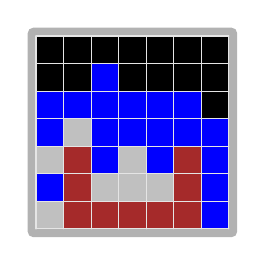
\begin{tikzpicture}
% TikZ grid exported from MARA
\def\cellsz{0.35cm}
\providecommand{\maraGridLineColor}{black!10}
\providecommand{\maraGridBorderColor}{black!30}
\providecommand{\maraGridLineWidth}{0.4pt}
\providecommand{\maraBorderLineWidth}{3pt}
\providecommand{\maraBorderRadius}{2pt}
\begin{scope}[x=\cellsz, y=\cellsz, line cap=round, line join=round]
  % Outer frame as a filled ring expanded by border line width with rounded corners
  \path[fill=\maraGridBorderColor, rounded corners=\maraBorderRadius] ([xshift=-\maraBorderLineWidth,yshift=-\maraBorderLineWidth]0,0) rectangle ([xshift=\maraBorderLineWidth,yshift=\maraBorderLineWidth]7,7);
  % Background
  \fill[black] (0,0) rectangle (7,7);
  % Filled cells
  \begin{scope}[fill={rgb,1:red,0.000;green,0.000;blue,1.000}, fill opacity=1.000]
    \fill (2,5) rectangle ++(1,1);
    \fill (0,4) rectangle ++(1,1);
    \fill (1,4) rectangle ++(1,1);
    \fill (2,4) rectangle ++(1,1);
    \fill (3,4) rectangle ++(1,1);
    \fill (4,4) rectangle ++(1,1);
    \fill (5,4) rectangle ++(1,1);
    \fill (0,3) rectangle ++(1,1);
    \fill (2,3) rectangle ++(1,1);
    \fill (3,3) rectangle ++(1,1);
    \fill (4,3) rectangle ++(1,1);
    \fill (5,3) rectangle ++(1,1);
    \fill (6,3) rectangle ++(1,1);
    \fill (2,2) rectangle ++(1,1);
    \fill (4,2) rectangle ++(1,1);
    \fill (6,2) rectangle ++(1,1);
    \fill (0,1) rectangle ++(1,1);
    \fill (6,1) rectangle ++(1,1);
    \fill (6,0) rectangle ++(1,1);
  \end{scope}
  \begin{scope}[fill={rgb,1:red,0.753;green,0.753;blue,0.753}, fill opacity=1.000]
    \fill (1,3) rectangle ++(1,1);
    \fill (0,2) rectangle ++(1,1);
    \fill (3,2) rectangle ++(1,1);
    \fill (2,1) rectangle ++(1,1);
    \fill (3,1) rectangle ++(1,1);
    \fill (4,1) rectangle ++(1,1);
    \fill (0,0) rectangle ++(1,1);
  \end{scope}
  \begin{scope}[fill={rgb,1:red,0.647;green,0.165;blue,0.165}, fill opacity=1.000]
    \fill (1,2) rectangle ++(1,1);
    \fill (5,2) rectangle ++(1,1);
    \fill (1,1) rectangle ++(1,1);
    \fill (5,1) rectangle ++(1,1);
    \fill (1,0) rectangle ++(1,1);
    \fill (2,0) rectangle ++(1,1);
    \fill (3,0) rectangle ++(1,1);
    \fill (4,0) rectangle ++(1,1);
    \fill (5,0) rectangle ++(1,1);
  \end{scope}
  % Grid and outline
  % Vertical lines
  \begin{scope}[draw=\maraGridLineColor, line width=\maraGridLineWidth, line cap=round]
    \draw (0,0) -- (0,7);
    \draw (1,0) -- (1,7);
    \draw (2,0) -- (2,7);
    \draw (3,0) -- (3,7);
    \draw (4,0) -- (4,7);
    \draw (5,0) -- (5,7);
    \draw (6,0) -- (6,7);
    \draw (7,0) -- (7,7);
  \end{scope}
  % Horizontal lines
  \begin{scope}[draw=\maraGridLineColor, line width=\maraGridLineWidth, line cap=round]
    \draw (0,0) -- (7,0);
    \draw (0,1) -- (7,1);
    \draw (0,2) -- (7,2);
    \draw (0,3) -- (7,3);
    \draw (0,4) -- (7,4);
    \draw (0,5) -- (7,5);
    \draw (0,6) -- (7,6);
    \draw (0,7) -- (7,7);
  \end{scope}
\end{scope}
\end{tikzpicture}
\ActionSequence{\ActionItem{noop x1}}
\medskip
% Step 25: noop x1
\smallskip
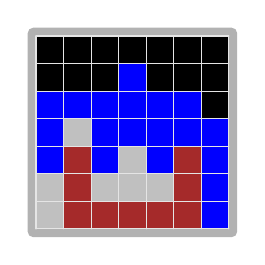
\begin{tikzpicture}
% TikZ grid exported from MARA
\def\cellsz{0.35cm}
\providecommand{\maraGridLineColor}{black!10}
\providecommand{\maraGridBorderColor}{black!30}
\providecommand{\maraGridLineWidth}{0.4pt}
\providecommand{\maraBorderLineWidth}{3pt}
\providecommand{\maraBorderRadius}{2pt}
\begin{scope}[x=\cellsz, y=\cellsz, line cap=round, line join=round]
  % Outer frame as a filled ring expanded by border line width with rounded corners
  \path[fill=\maraGridBorderColor, rounded corners=\maraBorderRadius] ([xshift=-\maraBorderLineWidth,yshift=-\maraBorderLineWidth]0,0) rectangle ([xshift=\maraBorderLineWidth,yshift=\maraBorderLineWidth]7,7);
  % Background
  \fill[black] (0,0) rectangle (7,7);
  % Filled cells
  \begin{scope}[fill={rgb,1:red,0.000;green,0.000;blue,1.000}, fill opacity=1.000]
    \fill (3,5) rectangle ++(1,1);
    \fill (0,4) rectangle ++(1,1);
    \fill (1,4) rectangle ++(1,1);
    \fill (2,4) rectangle ++(1,1);
    \fill (3,4) rectangle ++(1,1);
    \fill (4,4) rectangle ++(1,1);
    \fill (5,4) rectangle ++(1,1);
    \fill (0,3) rectangle ++(1,1);
    \fill (2,3) rectangle ++(1,1);
    \fill (3,3) rectangle ++(1,1);
    \fill (4,3) rectangle ++(1,1);
    \fill (5,3) rectangle ++(1,1);
    \fill (6,3) rectangle ++(1,1);
    \fill (0,2) rectangle ++(1,1);
    \fill (2,2) rectangle ++(1,1);
    \fill (4,2) rectangle ++(1,1);
    \fill (6,2) rectangle ++(1,1);
    \fill (6,1) rectangle ++(1,1);
    \fill (6,0) rectangle ++(1,1);
  \end{scope}
  \begin{scope}[fill={rgb,1:red,0.753;green,0.753;blue,0.753}, fill opacity=1.000]
    \fill (1,3) rectangle ++(1,1);
    \fill (3,2) rectangle ++(1,1);
    \fill (0,1) rectangle ++(1,1);
    \fill (2,1) rectangle ++(1,1);
    \fill (3,1) rectangle ++(1,1);
    \fill (4,1) rectangle ++(1,1);
    \fill (0,0) rectangle ++(1,1);
  \end{scope}
  \begin{scope}[fill={rgb,1:red,0.647;green,0.165;blue,0.165}, fill opacity=1.000]
    \fill (1,2) rectangle ++(1,1);
    \fill (5,2) rectangle ++(1,1);
    \fill (1,1) rectangle ++(1,1);
    \fill (5,1) rectangle ++(1,1);
    \fill (1,0) rectangle ++(1,1);
    \fill (2,0) rectangle ++(1,1);
    \fill (3,0) rectangle ++(1,1);
    \fill (4,0) rectangle ++(1,1);
    \fill (5,0) rectangle ++(1,1);
  \end{scope}
  % Grid and outline
  % Vertical lines
  \begin{scope}[draw=\maraGridLineColor, line width=\maraGridLineWidth, line cap=round]
    \draw (0,0) -- (0,7);
    \draw (1,0) -- (1,7);
    \draw (2,0) -- (2,7);
    \draw (3,0) -- (3,7);
    \draw (4,0) -- (4,7);
    \draw (5,0) -- (5,7);
    \draw (6,0) -- (6,7);
    \draw (7,0) -- (7,7);
  \end{scope}
  % Horizontal lines
  \begin{scope}[draw=\maraGridLineColor, line width=\maraGridLineWidth, line cap=round]
    \draw (0,0) -- (7,0);
    \draw (0,1) -- (7,1);
    \draw (0,2) -- (7,2);
    \draw (0,3) -- (7,3);
    \draw (0,4) -- (7,4);
    \draw (0,5) -- (7,5);
    \draw (0,6) -- (7,6);
    \draw (0,7) -- (7,7);
  \end{scope}
\end{scope}
\end{tikzpicture}
\ActionSequence{\ActionItem{noop x1}}
\medskip
% Step 26: click(0,0)
\smallskip
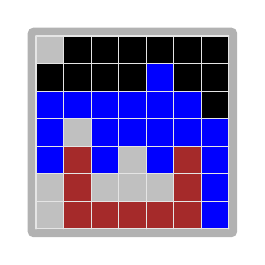
\begin{tikzpicture}
% TikZ grid exported from MARA
\def\cellsz{0.35cm}
\providecommand{\maraGridLineColor}{black!10}
\providecommand{\maraGridBorderColor}{black!30}
\providecommand{\maraGridLineWidth}{0.4pt}
\providecommand{\maraBorderLineWidth}{3pt}
\providecommand{\maraBorderRadius}{2pt}
\begin{scope}[x=\cellsz, y=\cellsz, line cap=round, line join=round]
  % Outer frame as a filled ring expanded by border line width with rounded corners
  \path[fill=\maraGridBorderColor, rounded corners=\maraBorderRadius] ([xshift=-\maraBorderLineWidth,yshift=-\maraBorderLineWidth]0,0) rectangle ([xshift=\maraBorderLineWidth,yshift=\maraBorderLineWidth]7,7);
  % Background
  \fill[black] (0,0) rectangle (7,7);
  % Filled cells
  \begin{scope}[fill={rgb,1:red,0.753;green,0.753;blue,0.753}, fill opacity=1.000]
    \fill (0,6) rectangle ++(1,1);
    \fill (1,3) rectangle ++(1,1);
    \fill (3,2) rectangle ++(1,1);
    \fill (0,1) rectangle ++(1,1);
    \fill (2,1) rectangle ++(1,1);
    \fill (3,1) rectangle ++(1,1);
    \fill (4,1) rectangle ++(1,1);
    \fill (0,0) rectangle ++(1,1);
  \end{scope}
  \begin{scope}[fill={rgb,1:red,0.000;green,0.000;blue,1.000}, fill opacity=1.000]
    \fill (4,5) rectangle ++(1,1);
    \fill (0,4) rectangle ++(1,1);
    \fill (1,4) rectangle ++(1,1);
    \fill (2,4) rectangle ++(1,1);
    \fill (3,4) rectangle ++(1,1);
    \fill (4,4) rectangle ++(1,1);
    \fill (5,4) rectangle ++(1,1);
    \fill (0,3) rectangle ++(1,1);
    \fill (2,3) rectangle ++(1,1);
    \fill (3,3) rectangle ++(1,1);
    \fill (4,3) rectangle ++(1,1);
    \fill (5,3) rectangle ++(1,1);
    \fill (6,3) rectangle ++(1,1);
    \fill (0,2) rectangle ++(1,1);
    \fill (2,2) rectangle ++(1,1);
    \fill (4,2) rectangle ++(1,1);
    \fill (6,2) rectangle ++(1,1);
    \fill (6,1) rectangle ++(1,1);
    \fill (6,0) rectangle ++(1,1);
  \end{scope}
  \begin{scope}[fill={rgb,1:red,0.647;green,0.165;blue,0.165}, fill opacity=1.000]
    \fill (1,2) rectangle ++(1,1);
    \fill (5,2) rectangle ++(1,1);
    \fill (1,1) rectangle ++(1,1);
    \fill (5,1) rectangle ++(1,1);
    \fill (1,0) rectangle ++(1,1);
    \fill (2,0) rectangle ++(1,1);
    \fill (3,0) rectangle ++(1,1);
    \fill (4,0) rectangle ++(1,1);
    \fill (5,0) rectangle ++(1,1);
  \end{scope}
  % Grid and outline
  % Vertical lines
  \begin{scope}[draw=\maraGridLineColor, line width=\maraGridLineWidth, line cap=round]
    \draw (0,0) -- (0,7);
    \draw (1,0) -- (1,7);
    \draw (2,0) -- (2,7);
    \draw (3,0) -- (3,7);
    \draw (4,0) -- (4,7);
    \draw (5,0) -- (5,7);
    \draw (6,0) -- (6,7);
    \draw (7,0) -- (7,7);
  \end{scope}
  % Horizontal lines
  \begin{scope}[draw=\maraGridLineColor, line width=\maraGridLineWidth, line cap=round]
    \draw (0,0) -- (7,0);
    \draw (0,1) -- (7,1);
    \draw (0,2) -- (7,2);
    \draw (0,3) -- (7,3);
    \draw (0,4) -- (7,4);
    \draw (0,5) -- (7,5);
    \draw (0,6) -- (7,6);
    \draw (0,7) -- (7,7);
  \end{scope}
\end{scope}
\end{tikzpicture}
\ActionSequence{\ActionItem{click(0,0)}}
\medskip
% Step 27: noop x1
\smallskip
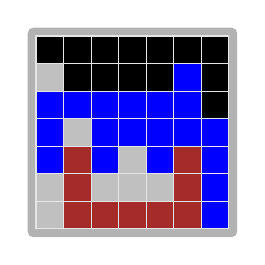
\begin{tikzpicture}
% TikZ grid exported from MARA
\def\cellsz{0.35cm}
\providecommand{\maraGridLineColor}{black!10}
\providecommand{\maraGridBorderColor}{black!30}
\providecommand{\maraGridLineWidth}{0.4pt}
\providecommand{\maraBorderLineWidth}{3pt}
\providecommand{\maraBorderRadius}{2pt}
\begin{scope}[x=\cellsz, y=\cellsz, line cap=round, line join=round]
  % Outer frame as a filled ring expanded by border line width with rounded corners
  \path[fill=\maraGridBorderColor, rounded corners=\maraBorderRadius] ([xshift=-\maraBorderLineWidth,yshift=-\maraBorderLineWidth]0,0) rectangle ([xshift=\maraBorderLineWidth,yshift=\maraBorderLineWidth]7,7);
  % Background
  \fill[black] (0,0) rectangle (7,7);
  % Filled cells
  \begin{scope}[fill={rgb,1:red,0.753;green,0.753;blue,0.753}, fill opacity=1.000]
    \fill (0,5) rectangle ++(1,1);
    \fill (1,3) rectangle ++(1,1);
    \fill (3,2) rectangle ++(1,1);
    \fill (0,1) rectangle ++(1,1);
    \fill (2,1) rectangle ++(1,1);
    \fill (3,1) rectangle ++(1,1);
    \fill (4,1) rectangle ++(1,1);
    \fill (0,0) rectangle ++(1,1);
  \end{scope}
  \begin{scope}[fill={rgb,1:red,0.000;green,0.000;blue,1.000}, fill opacity=1.000]
    \fill (5,5) rectangle ++(1,1);
    \fill (0,4) rectangle ++(1,1);
    \fill (1,4) rectangle ++(1,1);
    \fill (2,4) rectangle ++(1,1);
    \fill (3,4) rectangle ++(1,1);
    \fill (4,4) rectangle ++(1,1);
    \fill (5,4) rectangle ++(1,1);
    \fill (0,3) rectangle ++(1,1);
    \fill (2,3) rectangle ++(1,1);
    \fill (3,3) rectangle ++(1,1);
    \fill (4,3) rectangle ++(1,1);
    \fill (5,3) rectangle ++(1,1);
    \fill (6,3) rectangle ++(1,1);
    \fill (0,2) rectangle ++(1,1);
    \fill (2,2) rectangle ++(1,1);
    \fill (4,2) rectangle ++(1,1);
    \fill (6,2) rectangle ++(1,1);
    \fill (6,1) rectangle ++(1,1);
    \fill (6,0) rectangle ++(1,1);
  \end{scope}
  \begin{scope}[fill={rgb,1:red,0.647;green,0.165;blue,0.165}, fill opacity=1.000]
    \fill (1,2) rectangle ++(1,1);
    \fill (5,2) rectangle ++(1,1);
    \fill (1,1) rectangle ++(1,1);
    \fill (5,1) rectangle ++(1,1);
    \fill (1,0) rectangle ++(1,1);
    \fill (2,0) rectangle ++(1,1);
    \fill (3,0) rectangle ++(1,1);
    \fill (4,0) rectangle ++(1,1);
    \fill (5,0) rectangle ++(1,1);
  \end{scope}
  % Grid and outline
  % Vertical lines
  \begin{scope}[draw=\maraGridLineColor, line width=\maraGridLineWidth, line cap=round]
    \draw (0,0) -- (0,7);
    \draw (1,0) -- (1,7);
    \draw (2,0) -- (2,7);
    \draw (3,0) -- (3,7);
    \draw (4,0) -- (4,7);
    \draw (5,0) -- (5,7);
    \draw (6,0) -- (6,7);
    \draw (7,0) -- (7,7);
  \end{scope}
  % Horizontal lines
  \begin{scope}[draw=\maraGridLineColor, line width=\maraGridLineWidth, line cap=round]
    \draw (0,0) -- (7,0);
    \draw (0,1) -- (7,1);
    \draw (0,2) -- (7,2);
    \draw (0,3) -- (7,3);
    \draw (0,4) -- (7,4);
    \draw (0,5) -- (7,5);
    \draw (0,6) -- (7,6);
    \draw (0,7) -- (7,7);
  \end{scope}
\end{scope}
\end{tikzpicture}
\ActionSequence{\ActionItem{noop x1}}
\medskip
% Step 28: noop x1
\smallskip
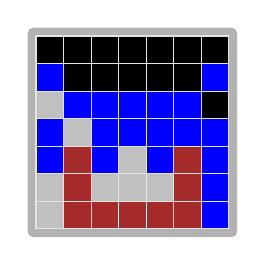
\begin{tikzpicture}
% TikZ grid exported from MARA
\def\cellsz{0.35cm}
\providecommand{\maraGridLineColor}{black!10}
\providecommand{\maraGridBorderColor}{black!30}
\providecommand{\maraGridLineWidth}{0.4pt}
\providecommand{\maraBorderLineWidth}{3pt}
\providecommand{\maraBorderRadius}{2pt}
\begin{scope}[x=\cellsz, y=\cellsz, line cap=round, line join=round]
  % Outer frame as a filled ring expanded by border line width with rounded corners
  \path[fill=\maraGridBorderColor, rounded corners=\maraBorderRadius] ([xshift=-\maraBorderLineWidth,yshift=-\maraBorderLineWidth]0,0) rectangle ([xshift=\maraBorderLineWidth,yshift=\maraBorderLineWidth]7,7);
  % Background
  \fill[black] (0,0) rectangle (7,7);
  % Filled cells
  \begin{scope}[fill={rgb,1:red,0.000;green,0.000;blue,1.000}, fill opacity=1.000]
    \fill (0,5) rectangle ++(1,1);
    \fill (6,5) rectangle ++(1,1);
    \fill (1,4) rectangle ++(1,1);
    \fill (2,4) rectangle ++(1,1);
    \fill (3,4) rectangle ++(1,1);
    \fill (4,4) rectangle ++(1,1);
    \fill (5,4) rectangle ++(1,1);
    \fill (0,3) rectangle ++(1,1);
    \fill (2,3) rectangle ++(1,1);
    \fill (3,3) rectangle ++(1,1);
    \fill (4,3) rectangle ++(1,1);
    \fill (5,3) rectangle ++(1,1);
    \fill (6,3) rectangle ++(1,1);
    \fill (0,2) rectangle ++(1,1);
    \fill (2,2) rectangle ++(1,1);
    \fill (4,2) rectangle ++(1,1);
    \fill (6,2) rectangle ++(1,1);
    \fill (6,1) rectangle ++(1,1);
    \fill (6,0) rectangle ++(1,1);
  \end{scope}
  \begin{scope}[fill={rgb,1:red,0.753;green,0.753;blue,0.753}, fill opacity=1.000]
    \fill (0,4) rectangle ++(1,1);
    \fill (1,3) rectangle ++(1,1);
    \fill (3,2) rectangle ++(1,1);
    \fill (0,1) rectangle ++(1,1);
    \fill (2,1) rectangle ++(1,1);
    \fill (3,1) rectangle ++(1,1);
    \fill (4,1) rectangle ++(1,1);
    \fill (0,0) rectangle ++(1,1);
  \end{scope}
  \begin{scope}[fill={rgb,1:red,0.647;green,0.165;blue,0.165}, fill opacity=1.000]
    \fill (1,2) rectangle ++(1,1);
    \fill (5,2) rectangle ++(1,1);
    \fill (1,1) rectangle ++(1,1);
    \fill (5,1) rectangle ++(1,1);
    \fill (1,0) rectangle ++(1,1);
    \fill (2,0) rectangle ++(1,1);
    \fill (3,0) rectangle ++(1,1);
    \fill (4,0) rectangle ++(1,1);
    \fill (5,0) rectangle ++(1,1);
  \end{scope}
  % Grid and outline
  % Vertical lines
  \begin{scope}[draw=\maraGridLineColor, line width=\maraGridLineWidth, line cap=round]
    \draw (0,0) -- (0,7);
    \draw (1,0) -- (1,7);
    \draw (2,0) -- (2,7);
    \draw (3,0) -- (3,7);
    \draw (4,0) -- (4,7);
    \draw (5,0) -- (5,7);
    \draw (6,0) -- (6,7);
    \draw (7,0) -- (7,7);
  \end{scope}
  % Horizontal lines
  \begin{scope}[draw=\maraGridLineColor, line width=\maraGridLineWidth, line cap=round]
    \draw (0,0) -- (7,0);
    \draw (0,1) -- (7,1);
    \draw (0,2) -- (7,2);
    \draw (0,3) -- (7,3);
    \draw (0,4) -- (7,4);
    \draw (0,5) -- (7,5);
    \draw (0,6) -- (7,6);
    \draw (0,7) -- (7,7);
  \end{scope}
\end{scope}
\end{tikzpicture}
\ActionSequence{\ActionItem{noop x1}}
\medskip
% Step 29: noop x1
\smallskip
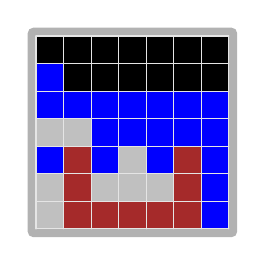
\begin{tikzpicture}
% TikZ grid exported from MARA
\def\cellsz{0.35cm}
\providecommand{\maraGridLineColor}{black!10}
\providecommand{\maraGridBorderColor}{black!30}
\providecommand{\maraGridLineWidth}{0.4pt}
\providecommand{\maraBorderLineWidth}{3pt}
\providecommand{\maraBorderRadius}{2pt}
\begin{scope}[x=\cellsz, y=\cellsz, line cap=round, line join=round]
  % Outer frame as a filled ring expanded by border line width with rounded corners
  \path[fill=\maraGridBorderColor, rounded corners=\maraBorderRadius] ([xshift=-\maraBorderLineWidth,yshift=-\maraBorderLineWidth]0,0) rectangle ([xshift=\maraBorderLineWidth,yshift=\maraBorderLineWidth]7,7);
  % Background
  \fill[black] (0,0) rectangle (7,7);
  % Filled cells
  \begin{scope}[fill={rgb,1:red,0.000;green,0.000;blue,1.000}, fill opacity=1.000]
    \fill (0,5) rectangle ++(1,1);
    \fill (0,4) rectangle ++(1,1);
    \fill (1,4) rectangle ++(1,1);
    \fill (2,4) rectangle ++(1,1);
    \fill (3,4) rectangle ++(1,1);
    \fill (4,4) rectangle ++(1,1);
    \fill (5,4) rectangle ++(1,1);
    \fill (6,4) rectangle ++(1,1);
    \fill (2,3) rectangle ++(1,1);
    \fill (3,3) rectangle ++(1,1);
    \fill (4,3) rectangle ++(1,1);
    \fill (5,3) rectangle ++(1,1);
    \fill (6,3) rectangle ++(1,1);
    \fill (0,2) rectangle ++(1,1);
    \fill (2,2) rectangle ++(1,1);
    \fill (4,2) rectangle ++(1,1);
    \fill (6,2) rectangle ++(1,1);
    \fill (6,1) rectangle ++(1,1);
    \fill (6,0) rectangle ++(1,1);
  \end{scope}
  \begin{scope}[fill={rgb,1:red,0.753;green,0.753;blue,0.753}, fill opacity=1.000]
    \fill (0,3) rectangle ++(1,1);
    \fill (1,3) rectangle ++(1,1);
    \fill (3,2) rectangle ++(1,1);
    \fill (0,1) rectangle ++(1,1);
    \fill (2,1) rectangle ++(1,1);
    \fill (3,1) rectangle ++(1,1);
    \fill (4,1) rectangle ++(1,1);
    \fill (0,0) rectangle ++(1,1);
  \end{scope}
  \begin{scope}[fill={rgb,1:red,0.647;green,0.165;blue,0.165}, fill opacity=1.000]
    \fill (1,2) rectangle ++(1,1);
    \fill (5,2) rectangle ++(1,1);
    \fill (1,1) rectangle ++(1,1);
    \fill (5,1) rectangle ++(1,1);
    \fill (1,0) rectangle ++(1,1);
    \fill (2,0) rectangle ++(1,1);
    \fill (3,0) rectangle ++(1,1);
    \fill (4,0) rectangle ++(1,1);
    \fill (5,0) rectangle ++(1,1);
  \end{scope}
  % Grid and outline
  % Vertical lines
  \begin{scope}[draw=\maraGridLineColor, line width=\maraGridLineWidth, line cap=round]
    \draw (0,0) -- (0,7);
    \draw (1,0) -- (1,7);
    \draw (2,0) -- (2,7);
    \draw (3,0) -- (3,7);
    \draw (4,0) -- (4,7);
    \draw (5,0) -- (5,7);
    \draw (6,0) -- (6,7);
    \draw (7,0) -- (7,7);
  \end{scope}
  % Horizontal lines
  \begin{scope}[draw=\maraGridLineColor, line width=\maraGridLineWidth, line cap=round]
    \draw (0,0) -- (7,0);
    \draw (0,1) -- (7,1);
    \draw (0,2) -- (7,2);
    \draw (0,3) -- (7,3);
    \draw (0,4) -- (7,4);
    \draw (0,5) -- (7,5);
    \draw (0,6) -- (7,6);
    \draw (0,7) -- (7,7);
  \end{scope}
\end{scope}
\end{tikzpicture}
\ActionSequence{\ActionItem{noop x1}}
\medskip
% Step 30: noop x4
\smallskip
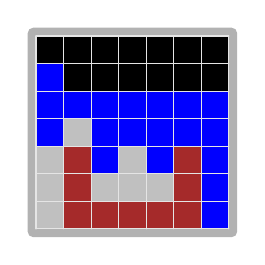
\begin{tikzpicture}
% TikZ grid exported from MARA
\def\cellsz{0.35cm}
\providecommand{\maraGridLineColor}{black!10}
\providecommand{\maraGridBorderColor}{black!30}
\providecommand{\maraGridLineWidth}{0.4pt}
\providecommand{\maraBorderLineWidth}{3pt}
\providecommand{\maraBorderRadius}{2pt}
\begin{scope}[x=\cellsz, y=\cellsz, line cap=round, line join=round]
  % Outer frame as a filled ring expanded by border line width with rounded corners
  \path[fill=\maraGridBorderColor, rounded corners=\maraBorderRadius] ([xshift=-\maraBorderLineWidth,yshift=-\maraBorderLineWidth]0,0) rectangle ([xshift=\maraBorderLineWidth,yshift=\maraBorderLineWidth]7,7);
  % Background
  \fill[black] (0,0) rectangle (7,7);
  % Filled cells
  \begin{scope}[fill={rgb,1:red,0.000;green,0.000;blue,1.000}, fill opacity=1.000]
    \fill (0,5) rectangle ++(1,1);
    \fill (0,4) rectangle ++(1,1);
    \fill (1,4) rectangle ++(1,1);
    \fill (2,4) rectangle ++(1,1);
    \fill (3,4) rectangle ++(1,1);
    \fill (4,4) rectangle ++(1,1);
    \fill (5,4) rectangle ++(1,1);
    \fill (6,4) rectangle ++(1,1);
    \fill (0,3) rectangle ++(1,1);
    \fill (2,3) rectangle ++(1,1);
    \fill (3,3) rectangle ++(1,1);
    \fill (4,3) rectangle ++(1,1);
    \fill (5,3) rectangle ++(1,1);
    \fill (6,3) rectangle ++(1,1);
    \fill (2,2) rectangle ++(1,1);
    \fill (4,2) rectangle ++(1,1);
    \fill (6,2) rectangle ++(1,1);
    \fill (6,1) rectangle ++(1,1);
    \fill (6,0) rectangle ++(1,1);
  \end{scope}
  \begin{scope}[fill={rgb,1:red,0.753;green,0.753;blue,0.753}, fill opacity=1.000]
    \fill (1,3) rectangle ++(1,1);
    \fill (0,2) rectangle ++(1,1);
    \fill (3,2) rectangle ++(1,1);
    \fill (0,1) rectangle ++(1,1);
    \fill (2,1) rectangle ++(1,1);
    \fill (3,1) rectangle ++(1,1);
    \fill (4,1) rectangle ++(1,1);
    \fill (0,0) rectangle ++(1,1);
  \end{scope}
  \begin{scope}[fill={rgb,1:red,0.647;green,0.165;blue,0.165}, fill opacity=1.000]
    \fill (1,2) rectangle ++(1,1);
    \fill (5,2) rectangle ++(1,1);
    \fill (1,1) rectangle ++(1,1);
    \fill (5,1) rectangle ++(1,1);
    \fill (1,0) rectangle ++(1,1);
    \fill (2,0) rectangle ++(1,1);
    \fill (3,0) rectangle ++(1,1);
    \fill (4,0) rectangle ++(1,1);
    \fill (5,0) rectangle ++(1,1);
  \end{scope}
  % Grid and outline
  % Vertical lines
  \begin{scope}[draw=\maraGridLineColor, line width=\maraGridLineWidth, line cap=round]
    \draw (0,0) -- (0,7);
    \draw (1,0) -- (1,7);
    \draw (2,0) -- (2,7);
    \draw (3,0) -- (3,7);
    \draw (4,0) -- (4,7);
    \draw (5,0) -- (5,7);
    \draw (6,0) -- (6,7);
    \draw (7,0) -- (7,7);
  \end{scope}
  % Horizontal lines
  \begin{scope}[draw=\maraGridLineColor, line width=\maraGridLineWidth, line cap=round]
    \draw (0,0) -- (7,0);
    \draw (0,1) -- (7,1);
    \draw (0,2) -- (7,2);
    \draw (0,3) -- (7,3);
    \draw (0,4) -- (7,4);
    \draw (0,5) -- (7,5);
    \draw (0,6) -- (7,6);
    \draw (0,7) -- (7,7);
  \end{scope}
\end{scope}
\end{tikzpicture}
\ActionSequence{\ActionItem{noop x4}}
\medskip
% Step 31: reset, noop x12
\smallskip
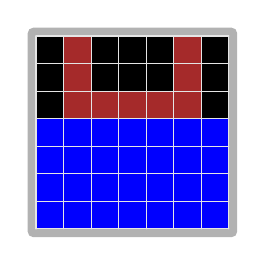
\begin{tikzpicture}
% TikZ grid exported from MARA
\def\cellsz{0.35cm}
\providecommand{\maraGridLineColor}{black!10}
\providecommand{\maraGridBorderColor}{black!30}
\providecommand{\maraGridLineWidth}{0.4pt}
\providecommand{\maraBorderLineWidth}{3pt}
\providecommand{\maraBorderRadius}{2pt}
\begin{scope}[x=\cellsz, y=\cellsz, line cap=round, line join=round]
  % Outer frame as a filled ring expanded by border line width with rounded corners
  \path[fill=\maraGridBorderColor, rounded corners=\maraBorderRadius] ([xshift=-\maraBorderLineWidth,yshift=-\maraBorderLineWidth]0,0) rectangle ([xshift=\maraBorderLineWidth,yshift=\maraBorderLineWidth]7,7);
  % Background
  \fill[black] (0,0) rectangle (7,7);
  % Filled cells
  \begin{scope}[fill={rgb,1:red,0.647;green,0.165;blue,0.165}, fill opacity=1.000]
    \fill (1,6) rectangle ++(1,1);
    \fill (5,6) rectangle ++(1,1);
    \fill (1,5) rectangle ++(1,1);
    \fill (5,5) rectangle ++(1,1);
    \fill (1,4) rectangle ++(1,1);
    \fill (2,4) rectangle ++(1,1);
    \fill (3,4) rectangle ++(1,1);
    \fill (4,4) rectangle ++(1,1);
    \fill (5,4) rectangle ++(1,1);
  \end{scope}
  \begin{scope}[fill={rgb,1:red,0.000;green,0.000;blue,1.000}, fill opacity=1.000]
    \fill (0,3) rectangle ++(1,1);
    \fill (1,3) rectangle ++(1,1);
    \fill (2,3) rectangle ++(1,1);
    \fill (3,3) rectangle ++(1,1);
    \fill (4,3) rectangle ++(1,1);
    \fill (5,3) rectangle ++(1,1);
    \fill (6,3) rectangle ++(1,1);
    \fill (0,2) rectangle ++(1,1);
    \fill (1,2) rectangle ++(1,1);
    \fill (2,2) rectangle ++(1,1);
    \fill (3,2) rectangle ++(1,1);
    \fill (4,2) rectangle ++(1,1);
    \fill (5,2) rectangle ++(1,1);
    \fill (6,2) rectangle ++(1,1);
    \fill (0,1) rectangle ++(1,1);
    \fill (1,1) rectangle ++(1,1);
    \fill (2,1) rectangle ++(1,1);
    \fill (3,1) rectangle ++(1,1);
    \fill (4,1) rectangle ++(1,1);
    \fill (5,1) rectangle ++(1,1);
    \fill (6,1) rectangle ++(1,1);
    \fill (0,0) rectangle ++(1,1);
    \fill (1,0) rectangle ++(1,1);
    \fill (2,0) rectangle ++(1,1);
    \fill (3,0) rectangle ++(1,1);
    \fill (4,0) rectangle ++(1,1);
    \fill (5,0) rectangle ++(1,1);
    \fill (6,0) rectangle ++(1,1);
  \end{scope}
  % Grid and outline
  % Vertical lines
  \begin{scope}[draw=\maraGridLineColor, line width=\maraGridLineWidth, line cap=round]
    \draw (0,0) -- (0,7);
    \draw (1,0) -- (1,7);
    \draw (2,0) -- (2,7);
    \draw (3,0) -- (3,7);
    \draw (4,0) -- (4,7);
    \draw (5,0) -- (5,7);
    \draw (6,0) -- (6,7);
    \draw (7,0) -- (7,7);
  \end{scope}
  % Horizontal lines
  \begin{scope}[draw=\maraGridLineColor, line width=\maraGridLineWidth, line cap=round]
    \draw (0,0) -- (7,0);
    \draw (0,1) -- (7,1);
    \draw (0,2) -- (7,2);
    \draw (0,3) -- (7,3);
    \draw (0,4) -- (7,4);
    \draw (0,5) -- (7,5);
    \draw (0,6) -- (7,6);
    \draw (0,7) -- (7,7);
  \end{scope}
\end{scope}
\end{tikzpicture}
\ActionSequence{\ActionItem{reset}\ActionItem{noop x12}}
\medskip
% Step 32: click(6,1)
\smallskip
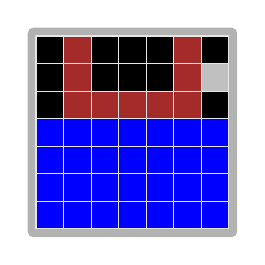
\begin{tikzpicture}
% TikZ grid exported from MARA
\def\cellsz{0.35cm}
\providecommand{\maraGridLineColor}{black!10}
\providecommand{\maraGridBorderColor}{black!30}
\providecommand{\maraGridLineWidth}{0.4pt}
\providecommand{\maraBorderLineWidth}{3pt}
\providecommand{\maraBorderRadius}{2pt}
\begin{scope}[x=\cellsz, y=\cellsz, line cap=round, line join=round]
  % Outer frame as a filled ring expanded by border line width with rounded corners
  \path[fill=\maraGridBorderColor, rounded corners=\maraBorderRadius] ([xshift=-\maraBorderLineWidth,yshift=-\maraBorderLineWidth]0,0) rectangle ([xshift=\maraBorderLineWidth,yshift=\maraBorderLineWidth]7,7);
  % Background
  \fill[black] (0,0) rectangle (7,7);
  % Filled cells
  \begin{scope}[fill={rgb,1:red,0.647;green,0.165;blue,0.165}, fill opacity=1.000]
    \fill (1,6) rectangle ++(1,1);
    \fill (5,6) rectangle ++(1,1);
    \fill (1,5) rectangle ++(1,1);
    \fill (5,5) rectangle ++(1,1);
    \fill (1,4) rectangle ++(1,1);
    \fill (2,4) rectangle ++(1,1);
    \fill (3,4) rectangle ++(1,1);
    \fill (4,4) rectangle ++(1,1);
    \fill (5,4) rectangle ++(1,1);
  \end{scope}
  \begin{scope}[fill={rgb,1:red,0.753;green,0.753;blue,0.753}, fill opacity=1.000]
    \fill (6,5) rectangle ++(1,1);
  \end{scope}
  \begin{scope}[fill={rgb,1:red,0.000;green,0.000;blue,1.000}, fill opacity=1.000]
    \fill (0,3) rectangle ++(1,1);
    \fill (1,3) rectangle ++(1,1);
    \fill (2,3) rectangle ++(1,1);
    \fill (3,3) rectangle ++(1,1);
    \fill (4,3) rectangle ++(1,1);
    \fill (5,3) rectangle ++(1,1);
    \fill (6,3) rectangle ++(1,1);
    \fill (0,2) rectangle ++(1,1);
    \fill (1,2) rectangle ++(1,1);
    \fill (2,2) rectangle ++(1,1);
    \fill (3,2) rectangle ++(1,1);
    \fill (4,2) rectangle ++(1,1);
    \fill (5,2) rectangle ++(1,1);
    \fill (6,2) rectangle ++(1,1);
    \fill (0,1) rectangle ++(1,1);
    \fill (1,1) rectangle ++(1,1);
    \fill (2,1) rectangle ++(1,1);
    \fill (3,1) rectangle ++(1,1);
    \fill (4,1) rectangle ++(1,1);
    \fill (5,1) rectangle ++(1,1);
    \fill (6,1) rectangle ++(1,1);
    \fill (0,0) rectangle ++(1,1);
    \fill (1,0) rectangle ++(1,1);
    \fill (2,0) rectangle ++(1,1);
    \fill (3,0) rectangle ++(1,1);
    \fill (4,0) rectangle ++(1,1);
    \fill (5,0) rectangle ++(1,1);
    \fill (6,0) rectangle ++(1,1);
  \end{scope}
  % Grid and outline
  % Vertical lines
  \begin{scope}[draw=\maraGridLineColor, line width=\maraGridLineWidth, line cap=round]
    \draw (0,0) -- (0,7);
    \draw (1,0) -- (1,7);
    \draw (2,0) -- (2,7);
    \draw (3,0) -- (3,7);
    \draw (4,0) -- (4,7);
    \draw (5,0) -- (5,7);
    \draw (6,0) -- (6,7);
    \draw (7,0) -- (7,7);
  \end{scope}
  % Horizontal lines
  \begin{scope}[draw=\maraGridLineColor, line width=\maraGridLineWidth, line cap=round]
    \draw (0,0) -- (7,0);
    \draw (0,1) -- (7,1);
    \draw (0,2) -- (7,2);
    \draw (0,3) -- (7,3);
    \draw (0,4) -- (7,4);
    \draw (0,5) -- (7,5);
    \draw (0,6) -- (7,6);
    \draw (0,7) -- (7,7);
  \end{scope}
\end{scope}
\end{tikzpicture}
\ActionSequence{\ActionItem{click(6,1)}}
\medskip
% Step 33: noop x1
\smallskip
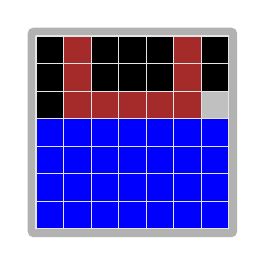
\begin{tikzpicture}
% TikZ grid exported from MARA
\def\cellsz{0.35cm}
\providecommand{\maraGridLineColor}{black!10}
\providecommand{\maraGridBorderColor}{black!30}
\providecommand{\maraGridLineWidth}{0.4pt}
\providecommand{\maraBorderLineWidth}{3pt}
\providecommand{\maraBorderRadius}{2pt}
\begin{scope}[x=\cellsz, y=\cellsz, line cap=round, line join=round]
  % Outer frame as a filled ring expanded by border line width with rounded corners
  \path[fill=\maraGridBorderColor, rounded corners=\maraBorderRadius] ([xshift=-\maraBorderLineWidth,yshift=-\maraBorderLineWidth]0,0) rectangle ([xshift=\maraBorderLineWidth,yshift=\maraBorderLineWidth]7,7);
  % Background
  \fill[black] (0,0) rectangle (7,7);
  % Filled cells
  \begin{scope}[fill={rgb,1:red,0.647;green,0.165;blue,0.165}, fill opacity=1.000]
    \fill (1,6) rectangle ++(1,1);
    \fill (5,6) rectangle ++(1,1);
    \fill (1,5) rectangle ++(1,1);
    \fill (5,5) rectangle ++(1,1);
    \fill (1,4) rectangle ++(1,1);
    \fill (2,4) rectangle ++(1,1);
    \fill (3,4) rectangle ++(1,1);
    \fill (4,4) rectangle ++(1,1);
    \fill (5,4) rectangle ++(1,1);
  \end{scope}
  \begin{scope}[fill={rgb,1:red,0.753;green,0.753;blue,0.753}, fill opacity=1.000]
    \fill (6,4) rectangle ++(1,1);
  \end{scope}
  \begin{scope}[fill={rgb,1:red,0.000;green,0.000;blue,1.000}, fill opacity=1.000]
    \fill (0,3) rectangle ++(1,1);
    \fill (1,3) rectangle ++(1,1);
    \fill (2,3) rectangle ++(1,1);
    \fill (3,3) rectangle ++(1,1);
    \fill (4,3) rectangle ++(1,1);
    \fill (5,3) rectangle ++(1,1);
    \fill (6,3) rectangle ++(1,1);
    \fill (0,2) rectangle ++(1,1);
    \fill (1,2) rectangle ++(1,1);
    \fill (2,2) rectangle ++(1,1);
    \fill (3,2) rectangle ++(1,1);
    \fill (4,2) rectangle ++(1,1);
    \fill (5,2) rectangle ++(1,1);
    \fill (6,2) rectangle ++(1,1);
    \fill (0,1) rectangle ++(1,1);
    \fill (1,1) rectangle ++(1,1);
    \fill (2,1) rectangle ++(1,1);
    \fill (3,1) rectangle ++(1,1);
    \fill (4,1) rectangle ++(1,1);
    \fill (5,1) rectangle ++(1,1);
    \fill (6,1) rectangle ++(1,1);
    \fill (0,0) rectangle ++(1,1);
    \fill (1,0) rectangle ++(1,1);
    \fill (2,0) rectangle ++(1,1);
    \fill (3,0) rectangle ++(1,1);
    \fill (4,0) rectangle ++(1,1);
    \fill (5,0) rectangle ++(1,1);
    \fill (6,0) rectangle ++(1,1);
  \end{scope}
  % Grid and outline
  % Vertical lines
  \begin{scope}[draw=\maraGridLineColor, line width=\maraGridLineWidth, line cap=round]
    \draw (0,0) -- (0,7);
    \draw (1,0) -- (1,7);
    \draw (2,0) -- (2,7);
    \draw (3,0) -- (3,7);
    \draw (4,0) -- (4,7);
    \draw (5,0) -- (5,7);
    \draw (6,0) -- (6,7);
    \draw (7,0) -- (7,7);
  \end{scope}
  % Horizontal lines
  \begin{scope}[draw=\maraGridLineColor, line width=\maraGridLineWidth, line cap=round]
    \draw (0,0) -- (7,0);
    \draw (0,1) -- (7,1);
    \draw (0,2) -- (7,2);
    \draw (0,3) -- (7,3);
    \draw (0,4) -- (7,4);
    \draw (0,5) -- (7,5);
    \draw (0,6) -- (7,6);
    \draw (0,7) -- (7,7);
  \end{scope}
\end{scope}
\end{tikzpicture}
\ActionSequence{\ActionItem{noop x1}}
\medskip
% Step 34: noop x1
\smallskip
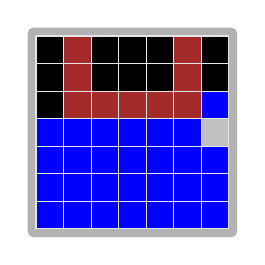
\begin{tikzpicture}
% TikZ grid exported from MARA
\def\cellsz{0.35cm}
\providecommand{\maraGridLineColor}{black!10}
\providecommand{\maraGridBorderColor}{black!30}
\providecommand{\maraGridLineWidth}{0.4pt}
\providecommand{\maraBorderLineWidth}{3pt}
\providecommand{\maraBorderRadius}{2pt}
\begin{scope}[x=\cellsz, y=\cellsz, line cap=round, line join=round]
  % Outer frame as a filled ring expanded by border line width with rounded corners
  \path[fill=\maraGridBorderColor, rounded corners=\maraBorderRadius] ([xshift=-\maraBorderLineWidth,yshift=-\maraBorderLineWidth]0,0) rectangle ([xshift=\maraBorderLineWidth,yshift=\maraBorderLineWidth]7,7);
  % Background
  \fill[black] (0,0) rectangle (7,7);
  % Filled cells
  \begin{scope}[fill={rgb,1:red,0.647;green,0.165;blue,0.165}, fill opacity=1.000]
    \fill (1,6) rectangle ++(1,1);
    \fill (5,6) rectangle ++(1,1);
    \fill (1,5) rectangle ++(1,1);
    \fill (5,5) rectangle ++(1,1);
    \fill (1,4) rectangle ++(1,1);
    \fill (2,4) rectangle ++(1,1);
    \fill (3,4) rectangle ++(1,1);
    \fill (4,4) rectangle ++(1,1);
    \fill (5,4) rectangle ++(1,1);
  \end{scope}
  \begin{scope}[fill={rgb,1:red,0.000;green,0.000;blue,1.000}, fill opacity=1.000]
    \fill (6,4) rectangle ++(1,1);
    \fill (0,3) rectangle ++(1,1);
    \fill (1,3) rectangle ++(1,1);
    \fill (2,3) rectangle ++(1,1);
    \fill (3,3) rectangle ++(1,1);
    \fill (4,3) rectangle ++(1,1);
    \fill (5,3) rectangle ++(1,1);
    \fill (0,2) rectangle ++(1,1);
    \fill (1,2) rectangle ++(1,1);
    \fill (2,2) rectangle ++(1,1);
    \fill (3,2) rectangle ++(1,1);
    \fill (4,2) rectangle ++(1,1);
    \fill (5,2) rectangle ++(1,1);
    \fill (6,2) rectangle ++(1,1);
    \fill (0,1) rectangle ++(1,1);
    \fill (1,1) rectangle ++(1,1);
    \fill (2,1) rectangle ++(1,1);
    \fill (3,1) rectangle ++(1,1);
    \fill (4,1) rectangle ++(1,1);
    \fill (5,1) rectangle ++(1,1);
    \fill (6,1) rectangle ++(1,1);
    \fill (0,0) rectangle ++(1,1);
    \fill (1,0) rectangle ++(1,1);
    \fill (2,0) rectangle ++(1,1);
    \fill (3,0) rectangle ++(1,1);
    \fill (4,0) rectangle ++(1,1);
    \fill (5,0) rectangle ++(1,1);
    \fill (6,0) rectangle ++(1,1);
  \end{scope}
  \begin{scope}[fill={rgb,1:red,0.753;green,0.753;blue,0.753}, fill opacity=1.000]
    \fill (6,3) rectangle ++(1,1);
  \end{scope}
  % Grid and outline
  % Vertical lines
  \begin{scope}[draw=\maraGridLineColor, line width=\maraGridLineWidth, line cap=round]
    \draw (0,0) -- (0,7);
    \draw (1,0) -- (1,7);
    \draw (2,0) -- (2,7);
    \draw (3,0) -- (3,7);
    \draw (4,0) -- (4,7);
    \draw (5,0) -- (5,7);
    \draw (6,0) -- (6,7);
    \draw (7,0) -- (7,7);
  \end{scope}
  % Horizontal lines
  \begin{scope}[draw=\maraGridLineColor, line width=\maraGridLineWidth, line cap=round]
    \draw (0,0) -- (7,0);
    \draw (0,1) -- (7,1);
    \draw (0,2) -- (7,2);
    \draw (0,3) -- (7,3);
    \draw (0,4) -- (7,4);
    \draw (0,5) -- (7,5);
    \draw (0,6) -- (7,6);
    \draw (0,7) -- (7,7);
  \end{scope}
\end{scope}
\end{tikzpicture}
\ActionSequence{\ActionItem{noop x1}}
\medskip
% Step 35: noop x1
\smallskip
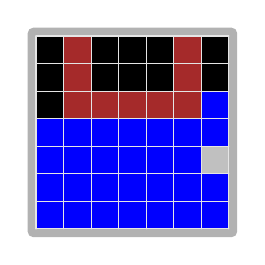
\begin{tikzpicture}
% TikZ grid exported from MARA
\def\cellsz{0.35cm}
\providecommand{\maraGridLineColor}{black!10}
\providecommand{\maraGridBorderColor}{black!30}
\providecommand{\maraGridLineWidth}{0.4pt}
\providecommand{\maraBorderLineWidth}{3pt}
\providecommand{\maraBorderRadius}{2pt}
\begin{scope}[x=\cellsz, y=\cellsz, line cap=round, line join=round]
  % Outer frame as a filled ring expanded by border line width with rounded corners
  \path[fill=\maraGridBorderColor, rounded corners=\maraBorderRadius] ([xshift=-\maraBorderLineWidth,yshift=-\maraBorderLineWidth]0,0) rectangle ([xshift=\maraBorderLineWidth,yshift=\maraBorderLineWidth]7,7);
  % Background
  \fill[black] (0,0) rectangle (7,7);
  % Filled cells
  \begin{scope}[fill={rgb,1:red,0.647;green,0.165;blue,0.165}, fill opacity=1.000]
    \fill (1,6) rectangle ++(1,1);
    \fill (5,6) rectangle ++(1,1);
    \fill (1,5) rectangle ++(1,1);
    \fill (5,5) rectangle ++(1,1);
    \fill (1,4) rectangle ++(1,1);
    \fill (2,4) rectangle ++(1,1);
    \fill (3,4) rectangle ++(1,1);
    \fill (4,4) rectangle ++(1,1);
    \fill (5,4) rectangle ++(1,1);
  \end{scope}
  \begin{scope}[fill={rgb,1:red,0.000;green,0.000;blue,1.000}, fill opacity=1.000]
    \fill (6,4) rectangle ++(1,1);
    \fill (0,3) rectangle ++(1,1);
    \fill (1,3) rectangle ++(1,1);
    \fill (2,3) rectangle ++(1,1);
    \fill (3,3) rectangle ++(1,1);
    \fill (4,3) rectangle ++(1,1);
    \fill (5,3) rectangle ++(1,1);
    \fill (6,3) rectangle ++(1,1);
    \fill (0,2) rectangle ++(1,1);
    \fill (1,2) rectangle ++(1,1);
    \fill (2,2) rectangle ++(1,1);
    \fill (3,2) rectangle ++(1,1);
    \fill (4,2) rectangle ++(1,1);
    \fill (5,2) rectangle ++(1,1);
    \fill (0,1) rectangle ++(1,1);
    \fill (1,1) rectangle ++(1,1);
    \fill (2,1) rectangle ++(1,1);
    \fill (3,1) rectangle ++(1,1);
    \fill (4,1) rectangle ++(1,1);
    \fill (5,1) rectangle ++(1,1);
    \fill (6,1) rectangle ++(1,1);
    \fill (0,0) rectangle ++(1,1);
    \fill (1,0) rectangle ++(1,1);
    \fill (2,0) rectangle ++(1,1);
    \fill (3,0) rectangle ++(1,1);
    \fill (4,0) rectangle ++(1,1);
    \fill (5,0) rectangle ++(1,1);
    \fill (6,0) rectangle ++(1,1);
  \end{scope}
  \begin{scope}[fill={rgb,1:red,0.753;green,0.753;blue,0.753}, fill opacity=1.000]
    \fill (6,2) rectangle ++(1,1);
  \end{scope}
  % Grid and outline
  % Vertical lines
  \begin{scope}[draw=\maraGridLineColor, line width=\maraGridLineWidth, line cap=round]
    \draw (0,0) -- (0,7);
    \draw (1,0) -- (1,7);
    \draw (2,0) -- (2,7);
    \draw (3,0) -- (3,7);
    \draw (4,0) -- (4,7);
    \draw (5,0) -- (5,7);
    \draw (6,0) -- (6,7);
    \draw (7,0) -- (7,7);
  \end{scope}
  % Horizontal lines
  \begin{scope}[draw=\maraGridLineColor, line width=\maraGridLineWidth, line cap=round]
    \draw (0,0) -- (7,0);
    \draw (0,1) -- (7,1);
    \draw (0,2) -- (7,2);
    \draw (0,3) -- (7,3);
    \draw (0,4) -- (7,4);
    \draw (0,5) -- (7,5);
    \draw (0,6) -- (7,6);
    \draw (0,7) -- (7,7);
  \end{scope}
\end{scope}
\end{tikzpicture}
\ActionSequence{\ActionItem{noop x1}}
\medskip
% Step 36: noop x1
\smallskip
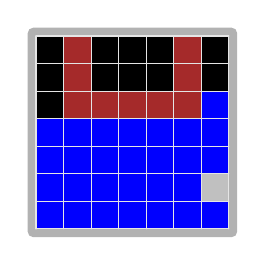
\begin{tikzpicture}
% TikZ grid exported from MARA
\def\cellsz{0.35cm}
\providecommand{\maraGridLineColor}{black!10}
\providecommand{\maraGridBorderColor}{black!30}
\providecommand{\maraGridLineWidth}{0.4pt}
\providecommand{\maraBorderLineWidth}{3pt}
\providecommand{\maraBorderRadius}{2pt}
\begin{scope}[x=\cellsz, y=\cellsz, line cap=round, line join=round]
  % Outer frame as a filled ring expanded by border line width with rounded corners
  \path[fill=\maraGridBorderColor, rounded corners=\maraBorderRadius] ([xshift=-\maraBorderLineWidth,yshift=-\maraBorderLineWidth]0,0) rectangle ([xshift=\maraBorderLineWidth,yshift=\maraBorderLineWidth]7,7);
  % Background
  \fill[black] (0,0) rectangle (7,7);
  % Filled cells
  \begin{scope}[fill={rgb,1:red,0.647;green,0.165;blue,0.165}, fill opacity=1.000]
    \fill (1,6) rectangle ++(1,1);
    \fill (5,6) rectangle ++(1,1);
    \fill (1,5) rectangle ++(1,1);
    \fill (5,5) rectangle ++(1,1);
    \fill (1,4) rectangle ++(1,1);
    \fill (2,4) rectangle ++(1,1);
    \fill (3,4) rectangle ++(1,1);
    \fill (4,4) rectangle ++(1,1);
    \fill (5,4) rectangle ++(1,1);
  \end{scope}
  \begin{scope}[fill={rgb,1:red,0.000;green,0.000;blue,1.000}, fill opacity=1.000]
    \fill (6,4) rectangle ++(1,1);
    \fill (0,3) rectangle ++(1,1);
    \fill (1,3) rectangle ++(1,1);
    \fill (2,3) rectangle ++(1,1);
    \fill (3,3) rectangle ++(1,1);
    \fill (4,3) rectangle ++(1,1);
    \fill (5,3) rectangle ++(1,1);
    \fill (6,3) rectangle ++(1,1);
    \fill (0,2) rectangle ++(1,1);
    \fill (1,2) rectangle ++(1,1);
    \fill (2,2) rectangle ++(1,1);
    \fill (3,2) rectangle ++(1,1);
    \fill (4,2) rectangle ++(1,1);
    \fill (5,2) rectangle ++(1,1);
    \fill (6,2) rectangle ++(1,1);
    \fill (0,1) rectangle ++(1,1);
    \fill (1,1) rectangle ++(1,1);
    \fill (2,1) rectangle ++(1,1);
    \fill (3,1) rectangle ++(1,1);
    \fill (4,1) rectangle ++(1,1);
    \fill (5,1) rectangle ++(1,1);
    \fill (0,0) rectangle ++(1,1);
    \fill (1,0) rectangle ++(1,1);
    \fill (2,0) rectangle ++(1,1);
    \fill (3,0) rectangle ++(1,1);
    \fill (4,0) rectangle ++(1,1);
    \fill (5,0) rectangle ++(1,1);
    \fill (6,0) rectangle ++(1,1);
  \end{scope}
  \begin{scope}[fill={rgb,1:red,0.753;green,0.753;blue,0.753}, fill opacity=1.000]
    \fill (6,1) rectangle ++(1,1);
  \end{scope}
  % Grid and outline
  % Vertical lines
  \begin{scope}[draw=\maraGridLineColor, line width=\maraGridLineWidth, line cap=round]
    \draw (0,0) -- (0,7);
    \draw (1,0) -- (1,7);
    \draw (2,0) -- (2,7);
    \draw (3,0) -- (3,7);
    \draw (4,0) -- (4,7);
    \draw (5,0) -- (5,7);
    \draw (6,0) -- (6,7);
    \draw (7,0) -- (7,7);
  \end{scope}
  % Horizontal lines
  \begin{scope}[draw=\maraGridLineColor, line width=\maraGridLineWidth, line cap=round]
    \draw (0,0) -- (7,0);
    \draw (0,1) -- (7,1);
    \draw (0,2) -- (7,2);
    \draw (0,3) -- (7,3);
    \draw (0,4) -- (7,4);
    \draw (0,5) -- (7,5);
    \draw (0,6) -- (7,6);
    \draw (0,7) -- (7,7);
  \end{scope}
\end{scope}
\end{tikzpicture}
\ActionSequence{\ActionItem{noop x1}}
\medskip
% Step 37: noop x8
\smallskip
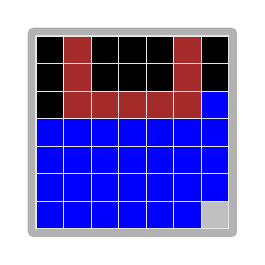
\begin{tikzpicture}
% TikZ grid exported from MARA
\def\cellsz{0.35cm}
\providecommand{\maraGridLineColor}{black!10}
\providecommand{\maraGridBorderColor}{black!30}
\providecommand{\maraGridLineWidth}{0.4pt}
\providecommand{\maraBorderLineWidth}{3pt}
\providecommand{\maraBorderRadius}{2pt}
\begin{scope}[x=\cellsz, y=\cellsz, line cap=round, line join=round]
  % Outer frame as a filled ring expanded by border line width with rounded corners
  \path[fill=\maraGridBorderColor, rounded corners=\maraBorderRadius] ([xshift=-\maraBorderLineWidth,yshift=-\maraBorderLineWidth]0,0) rectangle ([xshift=\maraBorderLineWidth,yshift=\maraBorderLineWidth]7,7);
  % Background
  \fill[black] (0,0) rectangle (7,7);
  % Filled cells
  \begin{scope}[fill={rgb,1:red,0.647;green,0.165;blue,0.165}, fill opacity=1.000]
    \fill (1,6) rectangle ++(1,1);
    \fill (5,6) rectangle ++(1,1);
    \fill (1,5) rectangle ++(1,1);
    \fill (5,5) rectangle ++(1,1);
    \fill (1,4) rectangle ++(1,1);
    \fill (2,4) rectangle ++(1,1);
    \fill (3,4) rectangle ++(1,1);
    \fill (4,4) rectangle ++(1,1);
    \fill (5,4) rectangle ++(1,1);
  \end{scope}
  \begin{scope}[fill={rgb,1:red,0.000;green,0.000;blue,1.000}, fill opacity=1.000]
    \fill (6,4) rectangle ++(1,1);
    \fill (0,3) rectangle ++(1,1);
    \fill (1,3) rectangle ++(1,1);
    \fill (2,3) rectangle ++(1,1);
    \fill (3,3) rectangle ++(1,1);
    \fill (4,3) rectangle ++(1,1);
    \fill (5,3) rectangle ++(1,1);
    \fill (6,3) rectangle ++(1,1);
    \fill (0,2) rectangle ++(1,1);
    \fill (1,2) rectangle ++(1,1);
    \fill (2,2) rectangle ++(1,1);
    \fill (3,2) rectangle ++(1,1);
    \fill (4,2) rectangle ++(1,1);
    \fill (5,2) rectangle ++(1,1);
    \fill (6,2) rectangle ++(1,1);
    \fill (0,1) rectangle ++(1,1);
    \fill (1,1) rectangle ++(1,1);
    \fill (2,1) rectangle ++(1,1);
    \fill (3,1) rectangle ++(1,1);
    \fill (4,1) rectangle ++(1,1);
    \fill (5,1) rectangle ++(1,1);
    \fill (6,1) rectangle ++(1,1);
    \fill (0,0) rectangle ++(1,1);
    \fill (1,0) rectangle ++(1,1);
    \fill (2,0) rectangle ++(1,1);
    \fill (3,0) rectangle ++(1,1);
    \fill (4,0) rectangle ++(1,1);
    \fill (5,0) rectangle ++(1,1);
  \end{scope}
  \begin{scope}[fill={rgb,1:red,0.753;green,0.753;blue,0.753}, fill opacity=1.000]
    \fill (6,0) rectangle ++(1,1);
  \end{scope}
  % Grid and outline
  % Vertical lines
  \begin{scope}[draw=\maraGridLineColor, line width=\maraGridLineWidth, line cap=round]
    \draw (0,0) -- (0,7);
    \draw (1,0) -- (1,7);
    \draw (2,0) -- (2,7);
    \draw (3,0) -- (3,7);
    \draw (4,0) -- (4,7);
    \draw (5,0) -- (5,7);
    \draw (6,0) -- (6,7);
    \draw (7,0) -- (7,7);
  \end{scope}
  % Horizontal lines
  \begin{scope}[draw=\maraGridLineColor, line width=\maraGridLineWidth, line cap=round]
    \draw (0,0) -- (7,0);
    \draw (0,1) -- (7,1);
    \draw (0,2) -- (7,2);
    \draw (0,3) -- (7,3);
    \draw (0,4) -- (7,4);
    \draw (0,5) -- (7,5);
    \draw (0,6) -- (7,6);
    \draw (0,7) -- (7,7);
  \end{scope}
\end{scope}
\end{tikzpicture}
\ActionSequence{\ActionItem{noop x8}}
\medskip
% Step 38: click(6,1)
\smallskip
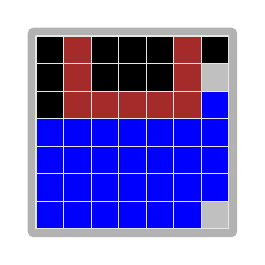
\begin{tikzpicture}
% TikZ grid exported from MARA
\def\cellsz{0.35cm}
\providecommand{\maraGridLineColor}{black!10}
\providecommand{\maraGridBorderColor}{black!30}
\providecommand{\maraGridLineWidth}{0.4pt}
\providecommand{\maraBorderLineWidth}{3pt}
\providecommand{\maraBorderRadius}{2pt}
\begin{scope}[x=\cellsz, y=\cellsz, line cap=round, line join=round]
  % Outer frame as a filled ring expanded by border line width with rounded corners
  \path[fill=\maraGridBorderColor, rounded corners=\maraBorderRadius] ([xshift=-\maraBorderLineWidth,yshift=-\maraBorderLineWidth]0,0) rectangle ([xshift=\maraBorderLineWidth,yshift=\maraBorderLineWidth]7,7);
  % Background
  \fill[black] (0,0) rectangle (7,7);
  % Filled cells
  \begin{scope}[fill={rgb,1:red,0.647;green,0.165;blue,0.165}, fill opacity=1.000]
    \fill (1,6) rectangle ++(1,1);
    \fill (5,6) rectangle ++(1,1);
    \fill (1,5) rectangle ++(1,1);
    \fill (5,5) rectangle ++(1,1);
    \fill (1,4) rectangle ++(1,1);
    \fill (2,4) rectangle ++(1,1);
    \fill (3,4) rectangle ++(1,1);
    \fill (4,4) rectangle ++(1,1);
    \fill (5,4) rectangle ++(1,1);
  \end{scope}
  \begin{scope}[fill={rgb,1:red,0.753;green,0.753;blue,0.753}, fill opacity=1.000]
    \fill (6,5) rectangle ++(1,1);
    \fill (6,0) rectangle ++(1,1);
  \end{scope}
  \begin{scope}[fill={rgb,1:red,0.000;green,0.000;blue,1.000}, fill opacity=1.000]
    \fill (6,4) rectangle ++(1,1);
    \fill (0,3) rectangle ++(1,1);
    \fill (1,3) rectangle ++(1,1);
    \fill (2,3) rectangle ++(1,1);
    \fill (3,3) rectangle ++(1,1);
    \fill (4,3) rectangle ++(1,1);
    \fill (5,3) rectangle ++(1,1);
    \fill (6,3) rectangle ++(1,1);
    \fill (0,2) rectangle ++(1,1);
    \fill (1,2) rectangle ++(1,1);
    \fill (2,2) rectangle ++(1,1);
    \fill (3,2) rectangle ++(1,1);
    \fill (4,2) rectangle ++(1,1);
    \fill (5,2) rectangle ++(1,1);
    \fill (6,2) rectangle ++(1,1);
    \fill (0,1) rectangle ++(1,1);
    \fill (1,1) rectangle ++(1,1);
    \fill (2,1) rectangle ++(1,1);
    \fill (3,1) rectangle ++(1,1);
    \fill (4,1) rectangle ++(1,1);
    \fill (5,1) rectangle ++(1,1);
    \fill (6,1) rectangle ++(1,1);
    \fill (0,0) rectangle ++(1,1);
    \fill (1,0) rectangle ++(1,1);
    \fill (2,0) rectangle ++(1,1);
    \fill (3,0) rectangle ++(1,1);
    \fill (4,0) rectangle ++(1,1);
    \fill (5,0) rectangle ++(1,1);
  \end{scope}
  % Grid and outline
  % Vertical lines
  \begin{scope}[draw=\maraGridLineColor, line width=\maraGridLineWidth, line cap=round]
    \draw (0,0) -- (0,7);
    \draw (1,0) -- (1,7);
    \draw (2,0) -- (2,7);
    \draw (3,0) -- (3,7);
    \draw (4,0) -- (4,7);
    \draw (5,0) -- (5,7);
    \draw (6,0) -- (6,7);
    \draw (7,0) -- (7,7);
  \end{scope}
  % Horizontal lines
  \begin{scope}[draw=\maraGridLineColor, line width=\maraGridLineWidth, line cap=round]
    \draw (0,0) -- (7,0);
    \draw (0,1) -- (7,1);
    \draw (0,2) -- (7,2);
    \draw (0,3) -- (7,3);
    \draw (0,4) -- (7,4);
    \draw (0,5) -- (7,5);
    \draw (0,6) -- (7,6);
    \draw (0,7) -- (7,7);
  \end{scope}
\end{scope}
\end{tikzpicture}
\ActionSequence{\ActionItem{click(6,1)}}
\medskip
% Step 39: noop x1
\smallskip
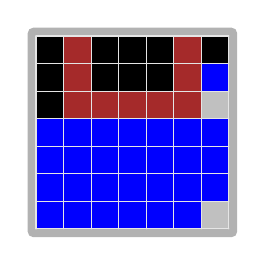
\begin{tikzpicture}
% TikZ grid exported from MARA
\def\cellsz{0.35cm}
\providecommand{\maraGridLineColor}{black!10}
\providecommand{\maraGridBorderColor}{black!30}
\providecommand{\maraGridLineWidth}{0.4pt}
\providecommand{\maraBorderLineWidth}{3pt}
\providecommand{\maraBorderRadius}{2pt}
\begin{scope}[x=\cellsz, y=\cellsz, line cap=round, line join=round]
  % Outer frame as a filled ring expanded by border line width with rounded corners
  \path[fill=\maraGridBorderColor, rounded corners=\maraBorderRadius] ([xshift=-\maraBorderLineWidth,yshift=-\maraBorderLineWidth]0,0) rectangle ([xshift=\maraBorderLineWidth,yshift=\maraBorderLineWidth]7,7);
  % Background
  \fill[black] (0,0) rectangle (7,7);
  % Filled cells
  \begin{scope}[fill={rgb,1:red,0.647;green,0.165;blue,0.165}, fill opacity=1.000]
    \fill (1,6) rectangle ++(1,1);
    \fill (5,6) rectangle ++(1,1);
    \fill (1,5) rectangle ++(1,1);
    \fill (5,5) rectangle ++(1,1);
    \fill (1,4) rectangle ++(1,1);
    \fill (2,4) rectangle ++(1,1);
    \fill (3,4) rectangle ++(1,1);
    \fill (4,4) rectangle ++(1,1);
    \fill (5,4) rectangle ++(1,1);
  \end{scope}
  \begin{scope}[fill={rgb,1:red,0.000;green,0.000;blue,1.000}, fill opacity=1.000]
    \fill (6,5) rectangle ++(1,1);
    \fill (0,3) rectangle ++(1,1);
    \fill (1,3) rectangle ++(1,1);
    \fill (2,3) rectangle ++(1,1);
    \fill (3,3) rectangle ++(1,1);
    \fill (4,3) rectangle ++(1,1);
    \fill (5,3) rectangle ++(1,1);
    \fill (6,3) rectangle ++(1,1);
    \fill (0,2) rectangle ++(1,1);
    \fill (1,2) rectangle ++(1,1);
    \fill (2,2) rectangle ++(1,1);
    \fill (3,2) rectangle ++(1,1);
    \fill (4,2) rectangle ++(1,1);
    \fill (5,2) rectangle ++(1,1);
    \fill (6,2) rectangle ++(1,1);
    \fill (0,1) rectangle ++(1,1);
    \fill (1,1) rectangle ++(1,1);
    \fill (2,1) rectangle ++(1,1);
    \fill (3,1) rectangle ++(1,1);
    \fill (4,1) rectangle ++(1,1);
    \fill (5,1) rectangle ++(1,1);
    \fill (6,1) rectangle ++(1,1);
    \fill (0,0) rectangle ++(1,1);
    \fill (1,0) rectangle ++(1,1);
    \fill (2,0) rectangle ++(1,1);
    \fill (3,0) rectangle ++(1,1);
    \fill (4,0) rectangle ++(1,1);
    \fill (5,0) rectangle ++(1,1);
  \end{scope}
  \begin{scope}[fill={rgb,1:red,0.753;green,0.753;blue,0.753}, fill opacity=1.000]
    \fill (6,4) rectangle ++(1,1);
    \fill (6,0) rectangle ++(1,1);
  \end{scope}
  % Grid and outline
  % Vertical lines
  \begin{scope}[draw=\maraGridLineColor, line width=\maraGridLineWidth, line cap=round]
    \draw (0,0) -- (0,7);
    \draw (1,0) -- (1,7);
    \draw (2,0) -- (2,7);
    \draw (3,0) -- (3,7);
    \draw (4,0) -- (4,7);
    \draw (5,0) -- (5,7);
    \draw (6,0) -- (6,7);
    \draw (7,0) -- (7,7);
  \end{scope}
  % Horizontal lines
  \begin{scope}[draw=\maraGridLineColor, line width=\maraGridLineWidth, line cap=round]
    \draw (0,0) -- (7,0);
    \draw (0,1) -- (7,1);
    \draw (0,2) -- (7,2);
    \draw (0,3) -- (7,3);
    \draw (0,4) -- (7,4);
    \draw (0,5) -- (7,5);
    \draw (0,6) -- (7,6);
    \draw (0,7) -- (7,7);
  \end{scope}
\end{scope}
\end{tikzpicture}
\ActionSequence{\ActionItem{noop x1}}
\medskip
% Step 40: noop x1
\smallskip
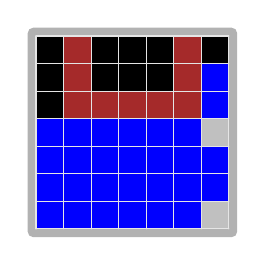
\begin{tikzpicture}
% TikZ grid exported from MARA
\def\cellsz{0.35cm}
\providecommand{\maraGridLineColor}{black!10}
\providecommand{\maraGridBorderColor}{black!30}
\providecommand{\maraGridLineWidth}{0.4pt}
\providecommand{\maraBorderLineWidth}{3pt}
\providecommand{\maraBorderRadius}{2pt}
\begin{scope}[x=\cellsz, y=\cellsz, line cap=round, line join=round]
  % Outer frame as a filled ring expanded by border line width with rounded corners
  \path[fill=\maraGridBorderColor, rounded corners=\maraBorderRadius] ([xshift=-\maraBorderLineWidth,yshift=-\maraBorderLineWidth]0,0) rectangle ([xshift=\maraBorderLineWidth,yshift=\maraBorderLineWidth]7,7);
  % Background
  \fill[black] (0,0) rectangle (7,7);
  % Filled cells
  \begin{scope}[fill={rgb,1:red,0.647;green,0.165;blue,0.165}, fill opacity=1.000]
    \fill (1,6) rectangle ++(1,1);
    \fill (5,6) rectangle ++(1,1);
    \fill (1,5) rectangle ++(1,1);
    \fill (5,5) rectangle ++(1,1);
    \fill (1,4) rectangle ++(1,1);
    \fill (2,4) rectangle ++(1,1);
    \fill (3,4) rectangle ++(1,1);
    \fill (4,4) rectangle ++(1,1);
    \fill (5,4) rectangle ++(1,1);
  \end{scope}
  \begin{scope}[fill={rgb,1:red,0.000;green,0.000;blue,1.000}, fill opacity=1.000]
    \fill (6,5) rectangle ++(1,1);
    \fill (6,4) rectangle ++(1,1);
    \fill (0,3) rectangle ++(1,1);
    \fill (1,3) rectangle ++(1,1);
    \fill (2,3) rectangle ++(1,1);
    \fill (3,3) rectangle ++(1,1);
    \fill (4,3) rectangle ++(1,1);
    \fill (5,3) rectangle ++(1,1);
    \fill (0,2) rectangle ++(1,1);
    \fill (1,2) rectangle ++(1,1);
    \fill (2,2) rectangle ++(1,1);
    \fill (3,2) rectangle ++(1,1);
    \fill (4,2) rectangle ++(1,1);
    \fill (5,2) rectangle ++(1,1);
    \fill (6,2) rectangle ++(1,1);
    \fill (0,1) rectangle ++(1,1);
    \fill (1,1) rectangle ++(1,1);
    \fill (2,1) rectangle ++(1,1);
    \fill (3,1) rectangle ++(1,1);
    \fill (4,1) rectangle ++(1,1);
    \fill (5,1) rectangle ++(1,1);
    \fill (6,1) rectangle ++(1,1);
    \fill (0,0) rectangle ++(1,1);
    \fill (1,0) rectangle ++(1,1);
    \fill (2,0) rectangle ++(1,1);
    \fill (3,0) rectangle ++(1,1);
    \fill (4,0) rectangle ++(1,1);
    \fill (5,0) rectangle ++(1,1);
  \end{scope}
  \begin{scope}[fill={rgb,1:red,0.753;green,0.753;blue,0.753}, fill opacity=1.000]
    \fill (6,3) rectangle ++(1,1);
    \fill (6,0) rectangle ++(1,1);
  \end{scope}
  % Grid and outline
  % Vertical lines
  \begin{scope}[draw=\maraGridLineColor, line width=\maraGridLineWidth, line cap=round]
    \draw (0,0) -- (0,7);
    \draw (1,0) -- (1,7);
    \draw (2,0) -- (2,7);
    \draw (3,0) -- (3,7);
    \draw (4,0) -- (4,7);
    \draw (5,0) -- (5,7);
    \draw (6,0) -- (6,7);
    \draw (7,0) -- (7,7);
  \end{scope}
  % Horizontal lines
  \begin{scope}[draw=\maraGridLineColor, line width=\maraGridLineWidth, line cap=round]
    \draw (0,0) -- (7,0);
    \draw (0,1) -- (7,1);
    \draw (0,2) -- (7,2);
    \draw (0,3) -- (7,3);
    \draw (0,4) -- (7,4);
    \draw (0,5) -- (7,5);
    \draw (0,6) -- (7,6);
    \draw (0,7) -- (7,7);
  \end{scope}
\end{scope}
\end{tikzpicture}
\ActionSequence{\ActionItem{noop x1}}
\medskip
% Step 41: noop x1
\smallskip
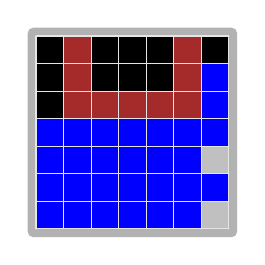
\begin{tikzpicture}
% TikZ grid exported from MARA
\def\cellsz{0.35cm}
\providecommand{\maraGridLineColor}{black!10}
\providecommand{\maraGridBorderColor}{black!30}
\providecommand{\maraGridLineWidth}{0.4pt}
\providecommand{\maraBorderLineWidth}{3pt}
\providecommand{\maraBorderRadius}{2pt}
\begin{scope}[x=\cellsz, y=\cellsz, line cap=round, line join=round]
  % Outer frame as a filled ring expanded by border line width with rounded corners
  \path[fill=\maraGridBorderColor, rounded corners=\maraBorderRadius] ([xshift=-\maraBorderLineWidth,yshift=-\maraBorderLineWidth]0,0) rectangle ([xshift=\maraBorderLineWidth,yshift=\maraBorderLineWidth]7,7);
  % Background
  \fill[black] (0,0) rectangle (7,7);
  % Filled cells
  \begin{scope}[fill={rgb,1:red,0.647;green,0.165;blue,0.165}, fill opacity=1.000]
    \fill (1,6) rectangle ++(1,1);
    \fill (5,6) rectangle ++(1,1);
    \fill (1,5) rectangle ++(1,1);
    \fill (5,5) rectangle ++(1,1);
    \fill (1,4) rectangle ++(1,1);
    \fill (2,4) rectangle ++(1,1);
    \fill (3,4) rectangle ++(1,1);
    \fill (4,4) rectangle ++(1,1);
    \fill (5,4) rectangle ++(1,1);
  \end{scope}
  \begin{scope}[fill={rgb,1:red,0.000;green,0.000;blue,1.000}, fill opacity=1.000]
    \fill (6,5) rectangle ++(1,1);
    \fill (6,4) rectangle ++(1,1);
    \fill (0,3) rectangle ++(1,1);
    \fill (1,3) rectangle ++(1,1);
    \fill (2,3) rectangle ++(1,1);
    \fill (3,3) rectangle ++(1,1);
    \fill (4,3) rectangle ++(1,1);
    \fill (5,3) rectangle ++(1,1);
    \fill (6,3) rectangle ++(1,1);
    \fill (0,2) rectangle ++(1,1);
    \fill (1,2) rectangle ++(1,1);
    \fill (2,2) rectangle ++(1,1);
    \fill (3,2) rectangle ++(1,1);
    \fill (4,2) rectangle ++(1,1);
    \fill (5,2) rectangle ++(1,1);
    \fill (0,1) rectangle ++(1,1);
    \fill (1,1) rectangle ++(1,1);
    \fill (2,1) rectangle ++(1,1);
    \fill (3,1) rectangle ++(1,1);
    \fill (4,1) rectangle ++(1,1);
    \fill (5,1) rectangle ++(1,1);
    \fill (6,1) rectangle ++(1,1);
    \fill (0,0) rectangle ++(1,1);
    \fill (1,0) rectangle ++(1,1);
    \fill (2,0) rectangle ++(1,1);
    \fill (3,0) rectangle ++(1,1);
    \fill (4,0) rectangle ++(1,1);
    \fill (5,0) rectangle ++(1,1);
  \end{scope}
  \begin{scope}[fill={rgb,1:red,0.753;green,0.753;blue,0.753}, fill opacity=1.000]
    \fill (6,2) rectangle ++(1,1);
    \fill (6,0) rectangle ++(1,1);
  \end{scope}
  % Grid and outline
  % Vertical lines
  \begin{scope}[draw=\maraGridLineColor, line width=\maraGridLineWidth, line cap=round]
    \draw (0,0) -- (0,7);
    \draw (1,0) -- (1,7);
    \draw (2,0) -- (2,7);
    \draw (3,0) -- (3,7);
    \draw (4,0) -- (4,7);
    \draw (5,0) -- (5,7);
    \draw (6,0) -- (6,7);
    \draw (7,0) -- (7,7);
  \end{scope}
  % Horizontal lines
  \begin{scope}[draw=\maraGridLineColor, line width=\maraGridLineWidth, line cap=round]
    \draw (0,0) -- (7,0);
    \draw (0,1) -- (7,1);
    \draw (0,2) -- (7,2);
    \draw (0,3) -- (7,3);
    \draw (0,4) -- (7,4);
    \draw (0,5) -- (7,5);
    \draw (0,6) -- (7,6);
    \draw (0,7) -- (7,7);
  \end{scope}
\end{scope}
\end{tikzpicture}
\ActionSequence{\ActionItem{noop x1}}
\medskip
% Step 42: noop x7, click(5,3), noop x7
\smallskip
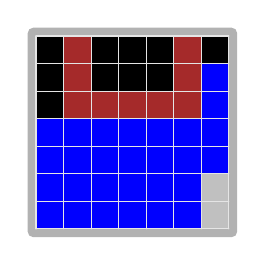
\begin{tikzpicture}
% TikZ grid exported from MARA
\def\cellsz{0.35cm}
\providecommand{\maraGridLineColor}{black!10}
\providecommand{\maraGridBorderColor}{black!30}
\providecommand{\maraGridLineWidth}{0.4pt}
\providecommand{\maraBorderLineWidth}{3pt}
\providecommand{\maraBorderRadius}{2pt}
\begin{scope}[x=\cellsz, y=\cellsz, line cap=round, line join=round]
  % Outer frame as a filled ring expanded by border line width with rounded corners
  \path[fill=\maraGridBorderColor, rounded corners=\maraBorderRadius] ([xshift=-\maraBorderLineWidth,yshift=-\maraBorderLineWidth]0,0) rectangle ([xshift=\maraBorderLineWidth,yshift=\maraBorderLineWidth]7,7);
  % Background
  \fill[black] (0,0) rectangle (7,7);
  % Filled cells
  \begin{scope}[fill={rgb,1:red,0.647;green,0.165;blue,0.165}, fill opacity=1.000]
    \fill (1,6) rectangle ++(1,1);
    \fill (5,6) rectangle ++(1,1);
    \fill (1,5) rectangle ++(1,1);
    \fill (5,5) rectangle ++(1,1);
    \fill (1,4) rectangle ++(1,1);
    \fill (2,4) rectangle ++(1,1);
    \fill (3,4) rectangle ++(1,1);
    \fill (4,4) rectangle ++(1,1);
    \fill (5,4) rectangle ++(1,1);
  \end{scope}
  \begin{scope}[fill={rgb,1:red,0.000;green,0.000;blue,1.000}, fill opacity=1.000]
    \fill (6,5) rectangle ++(1,1);
    \fill (6,4) rectangle ++(1,1);
    \fill (0,3) rectangle ++(1,1);
    \fill (1,3) rectangle ++(1,1);
    \fill (2,3) rectangle ++(1,1);
    \fill (3,3) rectangle ++(1,1);
    \fill (4,3) rectangle ++(1,1);
    \fill (5,3) rectangle ++(1,1);
    \fill (6,3) rectangle ++(1,1);
    \fill (0,2) rectangle ++(1,1);
    \fill (1,2) rectangle ++(1,1);
    \fill (2,2) rectangle ++(1,1);
    \fill (3,2) rectangle ++(1,1);
    \fill (4,2) rectangle ++(1,1);
    \fill (5,2) rectangle ++(1,1);
    \fill (6,2) rectangle ++(1,1);
    \fill (0,1) rectangle ++(1,1);
    \fill (1,1) rectangle ++(1,1);
    \fill (2,1) rectangle ++(1,1);
    \fill (3,1) rectangle ++(1,1);
    \fill (4,1) rectangle ++(1,1);
    \fill (5,1) rectangle ++(1,1);
    \fill (0,0) rectangle ++(1,1);
    \fill (1,0) rectangle ++(1,1);
    \fill (2,0) rectangle ++(1,1);
    \fill (3,0) rectangle ++(1,1);
    \fill (4,0) rectangle ++(1,1);
    \fill (5,0) rectangle ++(1,1);
  \end{scope}
  \begin{scope}[fill={rgb,1:red,0.753;green,0.753;blue,0.753}, fill opacity=1.000]
    \fill (6,1) rectangle ++(1,1);
    \fill (6,0) rectangle ++(1,1);
  \end{scope}
  % Grid and outline
  % Vertical lines
  \begin{scope}[draw=\maraGridLineColor, line width=\maraGridLineWidth, line cap=round]
    \draw (0,0) -- (0,7);
    \draw (1,0) -- (1,7);
    \draw (2,0) -- (2,7);
    \draw (3,0) -- (3,7);
    \draw (4,0) -- (4,7);
    \draw (5,0) -- (5,7);
    \draw (6,0) -- (6,7);
    \draw (7,0) -- (7,7);
  \end{scope}
  % Horizontal lines
  \begin{scope}[draw=\maraGridLineColor, line width=\maraGridLineWidth, line cap=round]
    \draw (0,0) -- (7,0);
    \draw (0,1) -- (7,1);
    \draw (0,2) -- (7,2);
    \draw (0,3) -- (7,3);
    \draw (0,4) -- (7,4);
    \draw (0,5) -- (7,5);
    \draw (0,6) -- (7,6);
    \draw (0,7) -- (7,7);
  \end{scope}
\end{scope}
\end{tikzpicture}
\ActionSequence{\ActionItem{noop x7}\ActionItem{click(5,3)}\ActionItem{noop x7}}
\medskip
% Step 43: click(0,2)
\smallskip
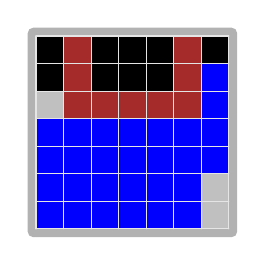
\begin{tikzpicture}
% TikZ grid exported from MARA
\def\cellsz{0.35cm}
\providecommand{\maraGridLineColor}{black!10}
\providecommand{\maraGridBorderColor}{black!30}
\providecommand{\maraGridLineWidth}{0.4pt}
\providecommand{\maraBorderLineWidth}{3pt}
\providecommand{\maraBorderRadius}{2pt}
\begin{scope}[x=\cellsz, y=\cellsz, line cap=round, line join=round]
  % Outer frame as a filled ring expanded by border line width with rounded corners
  \path[fill=\maraGridBorderColor, rounded corners=\maraBorderRadius] ([xshift=-\maraBorderLineWidth,yshift=-\maraBorderLineWidth]0,0) rectangle ([xshift=\maraBorderLineWidth,yshift=\maraBorderLineWidth]7,7);
  % Background
  \fill[black] (0,0) rectangle (7,7);
  % Filled cells
  \begin{scope}[fill={rgb,1:red,0.647;green,0.165;blue,0.165}, fill opacity=1.000]
    \fill (1,6) rectangle ++(1,1);
    \fill (5,6) rectangle ++(1,1);
    \fill (1,5) rectangle ++(1,1);
    \fill (5,5) rectangle ++(1,1);
    \fill (1,4) rectangle ++(1,1);
    \fill (2,4) rectangle ++(1,1);
    \fill (3,4) rectangle ++(1,1);
    \fill (4,4) rectangle ++(1,1);
    \fill (5,4) rectangle ++(1,1);
  \end{scope}
  \begin{scope}[fill={rgb,1:red,0.000;green,0.000;blue,1.000}, fill opacity=1.000]
    \fill (6,5) rectangle ++(1,1);
    \fill (6,4) rectangle ++(1,1);
    \fill (0,3) rectangle ++(1,1);
    \fill (1,3) rectangle ++(1,1);
    \fill (2,3) rectangle ++(1,1);
    \fill (3,3) rectangle ++(1,1);
    \fill (4,3) rectangle ++(1,1);
    \fill (5,3) rectangle ++(1,1);
    \fill (6,3) rectangle ++(1,1);
    \fill (0,2) rectangle ++(1,1);
    \fill (1,2) rectangle ++(1,1);
    \fill (2,2) rectangle ++(1,1);
    \fill (3,2) rectangle ++(1,1);
    \fill (4,2) rectangle ++(1,1);
    \fill (5,2) rectangle ++(1,1);
    \fill (6,2) rectangle ++(1,1);
    \fill (0,1) rectangle ++(1,1);
    \fill (1,1) rectangle ++(1,1);
    \fill (2,1) rectangle ++(1,1);
    \fill (3,1) rectangle ++(1,1);
    \fill (4,1) rectangle ++(1,1);
    \fill (5,1) rectangle ++(1,1);
    \fill (0,0) rectangle ++(1,1);
    \fill (1,0) rectangle ++(1,1);
    \fill (2,0) rectangle ++(1,1);
    \fill (3,0) rectangle ++(1,1);
    \fill (4,0) rectangle ++(1,1);
    \fill (5,0) rectangle ++(1,1);
  \end{scope}
  \begin{scope}[fill={rgb,1:red,0.753;green,0.753;blue,0.753}, fill opacity=1.000]
    \fill (0,4) rectangle ++(1,1);
    \fill (6,1) rectangle ++(1,1);
    \fill (6,0) rectangle ++(1,1);
  \end{scope}
  % Grid and outline
  % Vertical lines
  \begin{scope}[draw=\maraGridLineColor, line width=\maraGridLineWidth, line cap=round]
    \draw (0,0) -- (0,7);
    \draw (1,0) -- (1,7);
    \draw (2,0) -- (2,7);
    \draw (3,0) -- (3,7);
    \draw (4,0) -- (4,7);
    \draw (5,0) -- (5,7);
    \draw (6,0) -- (6,7);
    \draw (7,0) -- (7,7);
  \end{scope}
  % Horizontal lines
  \begin{scope}[draw=\maraGridLineColor, line width=\maraGridLineWidth, line cap=round]
    \draw (0,0) -- (7,0);
    \draw (0,1) -- (7,1);
    \draw (0,2) -- (7,2);
    \draw (0,3) -- (7,3);
    \draw (0,4) -- (7,4);
    \draw (0,5) -- (7,5);
    \draw (0,6) -- (7,6);
    \draw (0,7) -- (7,7);
  \end{scope}
\end{scope}
\end{tikzpicture}
\ActionSequence{\ActionItem{click(0,2)}}
\medskip
% Step 44: noop x1
\smallskip
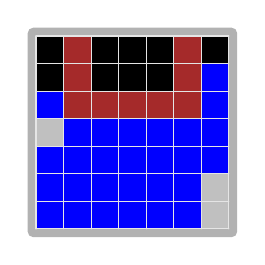
\begin{tikzpicture}
% TikZ grid exported from MARA
\def\cellsz{0.35cm}
\providecommand{\maraGridLineColor}{black!10}
\providecommand{\maraGridBorderColor}{black!30}
\providecommand{\maraGridLineWidth}{0.4pt}
\providecommand{\maraBorderLineWidth}{3pt}
\providecommand{\maraBorderRadius}{2pt}
\begin{scope}[x=\cellsz, y=\cellsz, line cap=round, line join=round]
  % Outer frame as a filled ring expanded by border line width with rounded corners
  \path[fill=\maraGridBorderColor, rounded corners=\maraBorderRadius] ([xshift=-\maraBorderLineWidth,yshift=-\maraBorderLineWidth]0,0) rectangle ([xshift=\maraBorderLineWidth,yshift=\maraBorderLineWidth]7,7);
  % Background
  \fill[black] (0,0) rectangle (7,7);
  % Filled cells
  \begin{scope}[fill={rgb,1:red,0.647;green,0.165;blue,0.165}, fill opacity=1.000]
    \fill (1,6) rectangle ++(1,1);
    \fill (5,6) rectangle ++(1,1);
    \fill (1,5) rectangle ++(1,1);
    \fill (5,5) rectangle ++(1,1);
    \fill (1,4) rectangle ++(1,1);
    \fill (2,4) rectangle ++(1,1);
    \fill (3,4) rectangle ++(1,1);
    \fill (4,4) rectangle ++(1,1);
    \fill (5,4) rectangle ++(1,1);
  \end{scope}
  \begin{scope}[fill={rgb,1:red,0.000;green,0.000;blue,1.000}, fill opacity=1.000]
    \fill (6,5) rectangle ++(1,1);
    \fill (0,4) rectangle ++(1,1);
    \fill (6,4) rectangle ++(1,1);
    \fill (1,3) rectangle ++(1,1);
    \fill (2,3) rectangle ++(1,1);
    \fill (3,3) rectangle ++(1,1);
    \fill (4,3) rectangle ++(1,1);
    \fill (5,3) rectangle ++(1,1);
    \fill (6,3) rectangle ++(1,1);
    \fill (0,2) rectangle ++(1,1);
    \fill (1,2) rectangle ++(1,1);
    \fill (2,2) rectangle ++(1,1);
    \fill (3,2) rectangle ++(1,1);
    \fill (4,2) rectangle ++(1,1);
    \fill (5,2) rectangle ++(1,1);
    \fill (6,2) rectangle ++(1,1);
    \fill (0,1) rectangle ++(1,1);
    \fill (1,1) rectangle ++(1,1);
    \fill (2,1) rectangle ++(1,1);
    \fill (3,1) rectangle ++(1,1);
    \fill (4,1) rectangle ++(1,1);
    \fill (5,1) rectangle ++(1,1);
    \fill (0,0) rectangle ++(1,1);
    \fill (1,0) rectangle ++(1,1);
    \fill (2,0) rectangle ++(1,1);
    \fill (3,0) rectangle ++(1,1);
    \fill (4,0) rectangle ++(1,1);
    \fill (5,0) rectangle ++(1,1);
  \end{scope}
  \begin{scope}[fill={rgb,1:red,0.753;green,0.753;blue,0.753}, fill opacity=1.000]
    \fill (0,3) rectangle ++(1,1);
    \fill (6,1) rectangle ++(1,1);
    \fill (6,0) rectangle ++(1,1);
  \end{scope}
  % Grid and outline
  % Vertical lines
  \begin{scope}[draw=\maraGridLineColor, line width=\maraGridLineWidth, line cap=round]
    \draw (0,0) -- (0,7);
    \draw (1,0) -- (1,7);
    \draw (2,0) -- (2,7);
    \draw (3,0) -- (3,7);
    \draw (4,0) -- (4,7);
    \draw (5,0) -- (5,7);
    \draw (6,0) -- (6,7);
    \draw (7,0) -- (7,7);
  \end{scope}
  % Horizontal lines
  \begin{scope}[draw=\maraGridLineColor, line width=\maraGridLineWidth, line cap=round]
    \draw (0,0) -- (7,0);
    \draw (0,1) -- (7,1);
    \draw (0,2) -- (7,2);
    \draw (0,3) -- (7,3);
    \draw (0,4) -- (7,4);
    \draw (0,5) -- (7,5);
    \draw (0,6) -- (7,6);
    \draw (0,7) -- (7,7);
  \end{scope}
\end{scope}
\end{tikzpicture}
\ActionSequence{\ActionItem{noop x1}}
\medskip
% Step 45: noop x1
\smallskip
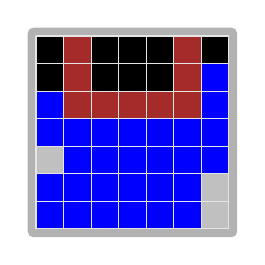
\begin{tikzpicture}
% TikZ grid exported from MARA
\def\cellsz{0.35cm}
\providecommand{\maraGridLineColor}{black!10}
\providecommand{\maraGridBorderColor}{black!30}
\providecommand{\maraGridLineWidth}{0.4pt}
\providecommand{\maraBorderLineWidth}{3pt}
\providecommand{\maraBorderRadius}{2pt}
\begin{scope}[x=\cellsz, y=\cellsz, line cap=round, line join=round]
  % Outer frame as a filled ring expanded by border line width with rounded corners
  \path[fill=\maraGridBorderColor, rounded corners=\maraBorderRadius] ([xshift=-\maraBorderLineWidth,yshift=-\maraBorderLineWidth]0,0) rectangle ([xshift=\maraBorderLineWidth,yshift=\maraBorderLineWidth]7,7);
  % Background
  \fill[black] (0,0) rectangle (7,7);
  % Filled cells
  \begin{scope}[fill={rgb,1:red,0.647;green,0.165;blue,0.165}, fill opacity=1.000]
    \fill (1,6) rectangle ++(1,1);
    \fill (5,6) rectangle ++(1,1);
    \fill (1,5) rectangle ++(1,1);
    \fill (5,5) rectangle ++(1,1);
    \fill (1,4) rectangle ++(1,1);
    \fill (2,4) rectangle ++(1,1);
    \fill (3,4) rectangle ++(1,1);
    \fill (4,4) rectangle ++(1,1);
    \fill (5,4) rectangle ++(1,1);
  \end{scope}
  \begin{scope}[fill={rgb,1:red,0.000;green,0.000;blue,1.000}, fill opacity=1.000]
    \fill (6,5) rectangle ++(1,1);
    \fill (0,4) rectangle ++(1,1);
    \fill (6,4) rectangle ++(1,1);
    \fill (0,3) rectangle ++(1,1);
    \fill (1,3) rectangle ++(1,1);
    \fill (2,3) rectangle ++(1,1);
    \fill (3,3) rectangle ++(1,1);
    \fill (4,3) rectangle ++(1,1);
    \fill (5,3) rectangle ++(1,1);
    \fill (6,3) rectangle ++(1,1);
    \fill (1,2) rectangle ++(1,1);
    \fill (2,2) rectangle ++(1,1);
    \fill (3,2) rectangle ++(1,1);
    \fill (4,2) rectangle ++(1,1);
    \fill (5,2) rectangle ++(1,1);
    \fill (6,2) rectangle ++(1,1);
    \fill (0,1) rectangle ++(1,1);
    \fill (1,1) rectangle ++(1,1);
    \fill (2,1) rectangle ++(1,1);
    \fill (3,1) rectangle ++(1,1);
    \fill (4,1) rectangle ++(1,1);
    \fill (5,1) rectangle ++(1,1);
    \fill (0,0) rectangle ++(1,1);
    \fill (1,0) rectangle ++(1,1);
    \fill (2,0) rectangle ++(1,1);
    \fill (3,0) rectangle ++(1,1);
    \fill (4,0) rectangle ++(1,1);
    \fill (5,0) rectangle ++(1,1);
  \end{scope}
  \begin{scope}[fill={rgb,1:red,0.753;green,0.753;blue,0.753}, fill opacity=1.000]
    \fill (0,2) rectangle ++(1,1);
    \fill (6,1) rectangle ++(1,1);
    \fill (6,0) rectangle ++(1,1);
  \end{scope}
  % Grid and outline
  % Vertical lines
  \begin{scope}[draw=\maraGridLineColor, line width=\maraGridLineWidth, line cap=round]
    \draw (0,0) -- (0,7);
    \draw (1,0) -- (1,7);
    \draw (2,0) -- (2,7);
    \draw (3,0) -- (3,7);
    \draw (4,0) -- (4,7);
    \draw (5,0) -- (5,7);
    \draw (6,0) -- (6,7);
    \draw (7,0) -- (7,7);
  \end{scope}
  % Horizontal lines
  \begin{scope}[draw=\maraGridLineColor, line width=\maraGridLineWidth, line cap=round]
    \draw (0,0) -- (7,0);
    \draw (0,1) -- (7,1);
    \draw (0,2) -- (7,2);
    \draw (0,3) -- (7,3);
    \draw (0,4) -- (7,4);
    \draw (0,5) -- (7,5);
    \draw (0,6) -- (7,6);
    \draw (0,7) -- (7,7);
  \end{scope}
\end{scope}
\end{tikzpicture}
\ActionSequence{\ActionItem{noop x1}}
\medskip
% Step 46: noop x1
\smallskip
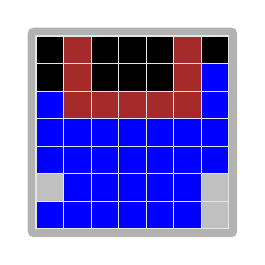
\begin{tikzpicture}
% TikZ grid exported from MARA
\def\cellsz{0.35cm}
\providecommand{\maraGridLineColor}{black!10}
\providecommand{\maraGridBorderColor}{black!30}
\providecommand{\maraGridLineWidth}{0.4pt}
\providecommand{\maraBorderLineWidth}{3pt}
\providecommand{\maraBorderRadius}{2pt}
\begin{scope}[x=\cellsz, y=\cellsz, line cap=round, line join=round]
  % Outer frame as a filled ring expanded by border line width with rounded corners
  \path[fill=\maraGridBorderColor, rounded corners=\maraBorderRadius] ([xshift=-\maraBorderLineWidth,yshift=-\maraBorderLineWidth]0,0) rectangle ([xshift=\maraBorderLineWidth,yshift=\maraBorderLineWidth]7,7);
  % Background
  \fill[black] (0,0) rectangle (7,7);
  % Filled cells
  \begin{scope}[fill={rgb,1:red,0.647;green,0.165;blue,0.165}, fill opacity=1.000]
    \fill (1,6) rectangle ++(1,1);
    \fill (5,6) rectangle ++(1,1);
    \fill (1,5) rectangle ++(1,1);
    \fill (5,5) rectangle ++(1,1);
    \fill (1,4) rectangle ++(1,1);
    \fill (2,4) rectangle ++(1,1);
    \fill (3,4) rectangle ++(1,1);
    \fill (4,4) rectangle ++(1,1);
    \fill (5,4) rectangle ++(1,1);
  \end{scope}
  \begin{scope}[fill={rgb,1:red,0.000;green,0.000;blue,1.000}, fill opacity=1.000]
    \fill (6,5) rectangle ++(1,1);
    \fill (0,4) rectangle ++(1,1);
    \fill (6,4) rectangle ++(1,1);
    \fill (0,3) rectangle ++(1,1);
    \fill (1,3) rectangle ++(1,1);
    \fill (2,3) rectangle ++(1,1);
    \fill (3,3) rectangle ++(1,1);
    \fill (4,3) rectangle ++(1,1);
    \fill (5,3) rectangle ++(1,1);
    \fill (6,3) rectangle ++(1,1);
    \fill (0,2) rectangle ++(1,1);
    \fill (1,2) rectangle ++(1,1);
    \fill (2,2) rectangle ++(1,1);
    \fill (3,2) rectangle ++(1,1);
    \fill (4,2) rectangle ++(1,1);
    \fill (5,2) rectangle ++(1,1);
    \fill (6,2) rectangle ++(1,1);
    \fill (1,1) rectangle ++(1,1);
    \fill (2,1) rectangle ++(1,1);
    \fill (3,1) rectangle ++(1,1);
    \fill (4,1) rectangle ++(1,1);
    \fill (5,1) rectangle ++(1,1);
    \fill (0,0) rectangle ++(1,1);
    \fill (1,0) rectangle ++(1,1);
    \fill (2,0) rectangle ++(1,1);
    \fill (3,0) rectangle ++(1,1);
    \fill (4,0) rectangle ++(1,1);
    \fill (5,0) rectangle ++(1,1);
  \end{scope}
  \begin{scope}[fill={rgb,1:red,0.753;green,0.753;blue,0.753}, fill opacity=1.000]
    \fill (0,1) rectangle ++(1,1);
    \fill (6,1) rectangle ++(1,1);
    \fill (6,0) rectangle ++(1,1);
  \end{scope}
  % Grid and outline
  % Vertical lines
  \begin{scope}[draw=\maraGridLineColor, line width=\maraGridLineWidth, line cap=round]
    \draw (0,0) -- (0,7);
    \draw (1,0) -- (1,7);
    \draw (2,0) -- (2,7);
    \draw (3,0) -- (3,7);
    \draw (4,0) -- (4,7);
    \draw (5,0) -- (5,7);
    \draw (6,0) -- (6,7);
    \draw (7,0) -- (7,7);
  \end{scope}
  % Horizontal lines
  \begin{scope}[draw=\maraGridLineColor, line width=\maraGridLineWidth, line cap=round]
    \draw (0,0) -- (7,0);
    \draw (0,1) -- (7,1);
    \draw (0,2) -- (7,2);
    \draw (0,3) -- (7,3);
    \draw (0,4) -- (7,4);
    \draw (0,5) -- (7,5);
    \draw (0,6) -- (7,6);
    \draw (0,7) -- (7,7);
  \end{scope}
\end{scope}
\end{tikzpicture}
\ActionSequence{\ActionItem{noop x1}}
\medskip
% Step 47: noop x8
\smallskip
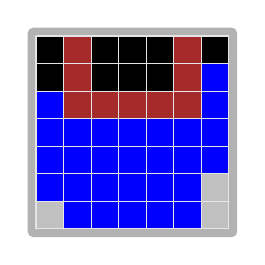
\begin{tikzpicture}
% TikZ grid exported from MARA
\def\cellsz{0.35cm}
\providecommand{\maraGridLineColor}{black!10}
\providecommand{\maraGridBorderColor}{black!30}
\providecommand{\maraGridLineWidth}{0.4pt}
\providecommand{\maraBorderLineWidth}{3pt}
\providecommand{\maraBorderRadius}{2pt}
\begin{scope}[x=\cellsz, y=\cellsz, line cap=round, line join=round]
  % Outer frame as a filled ring expanded by border line width with rounded corners
  \path[fill=\maraGridBorderColor, rounded corners=\maraBorderRadius] ([xshift=-\maraBorderLineWidth,yshift=-\maraBorderLineWidth]0,0) rectangle ([xshift=\maraBorderLineWidth,yshift=\maraBorderLineWidth]7,7);
  % Background
  \fill[black] (0,0) rectangle (7,7);
  % Filled cells
  \begin{scope}[fill={rgb,1:red,0.647;green,0.165;blue,0.165}, fill opacity=1.000]
    \fill (1,6) rectangle ++(1,1);
    \fill (5,6) rectangle ++(1,1);
    \fill (1,5) rectangle ++(1,1);
    \fill (5,5) rectangle ++(1,1);
    \fill (1,4) rectangle ++(1,1);
    \fill (2,4) rectangle ++(1,1);
    \fill (3,4) rectangle ++(1,1);
    \fill (4,4) rectangle ++(1,1);
    \fill (5,4) rectangle ++(1,1);
  \end{scope}
  \begin{scope}[fill={rgb,1:red,0.000;green,0.000;blue,1.000}, fill opacity=1.000]
    \fill (6,5) rectangle ++(1,1);
    \fill (0,4) rectangle ++(1,1);
    \fill (6,4) rectangle ++(1,1);
    \fill (0,3) rectangle ++(1,1);
    \fill (1,3) rectangle ++(1,1);
    \fill (2,3) rectangle ++(1,1);
    \fill (3,3) rectangle ++(1,1);
    \fill (4,3) rectangle ++(1,1);
    \fill (5,3) rectangle ++(1,1);
    \fill (6,3) rectangle ++(1,1);
    \fill (0,2) rectangle ++(1,1);
    \fill (1,2) rectangle ++(1,1);
    \fill (2,2) rectangle ++(1,1);
    \fill (3,2) rectangle ++(1,1);
    \fill (4,2) rectangle ++(1,1);
    \fill (5,2) rectangle ++(1,1);
    \fill (6,2) rectangle ++(1,1);
    \fill (0,1) rectangle ++(1,1);
    \fill (1,1) rectangle ++(1,1);
    \fill (2,1) rectangle ++(1,1);
    \fill (3,1) rectangle ++(1,1);
    \fill (4,1) rectangle ++(1,1);
    \fill (5,1) rectangle ++(1,1);
    \fill (1,0) rectangle ++(1,1);
    \fill (2,0) rectangle ++(1,1);
    \fill (3,0) rectangle ++(1,1);
    \fill (4,0) rectangle ++(1,1);
    \fill (5,0) rectangle ++(1,1);
  \end{scope}
  \begin{scope}[fill={rgb,1:red,0.753;green,0.753;blue,0.753}, fill opacity=1.000]
    \fill (6,1) rectangle ++(1,1);
    \fill (0,0) rectangle ++(1,1);
    \fill (6,0) rectangle ++(1,1);
  \end{scope}
  % Grid and outline
  % Vertical lines
  \begin{scope}[draw=\maraGridLineColor, line width=\maraGridLineWidth, line cap=round]
    \draw (0,0) -- (0,7);
    \draw (1,0) -- (1,7);
    \draw (2,0) -- (2,7);
    \draw (3,0) -- (3,7);
    \draw (4,0) -- (4,7);
    \draw (5,0) -- (5,7);
    \draw (6,0) -- (6,7);
    \draw (7,0) -- (7,7);
  \end{scope}
  % Horizontal lines
  \begin{scope}[draw=\maraGridLineColor, line width=\maraGridLineWidth, line cap=round]
    \draw (0,0) -- (7,0);
    \draw (0,1) -- (7,1);
    \draw (0,2) -- (7,2);
    \draw (0,3) -- (7,3);
    \draw (0,4) -- (7,4);
    \draw (0,5) -- (7,5);
    \draw (0,6) -- (7,6);
    \draw (0,7) -- (7,7);
  \end{scope}
\end{scope}
\end{tikzpicture}
\ActionSequence{\ActionItem{noop x8}}
\medskip
% Step 48: click(0,1)
\smallskip
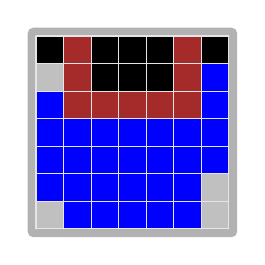
\begin{tikzpicture}
% TikZ grid exported from MARA
\def\cellsz{0.35cm}
\providecommand{\maraGridLineColor}{black!10}
\providecommand{\maraGridBorderColor}{black!30}
\providecommand{\maraGridLineWidth}{0.4pt}
\providecommand{\maraBorderLineWidth}{3pt}
\providecommand{\maraBorderRadius}{2pt}
\begin{scope}[x=\cellsz, y=\cellsz, line cap=round, line join=round]
  % Outer frame as a filled ring expanded by border line width with rounded corners
  \path[fill=\maraGridBorderColor, rounded corners=\maraBorderRadius] ([xshift=-\maraBorderLineWidth,yshift=-\maraBorderLineWidth]0,0) rectangle ([xshift=\maraBorderLineWidth,yshift=\maraBorderLineWidth]7,7);
  % Background
  \fill[black] (0,0) rectangle (7,7);
  % Filled cells
  \begin{scope}[fill={rgb,1:red,0.647;green,0.165;blue,0.165}, fill opacity=1.000]
    \fill (1,6) rectangle ++(1,1);
    \fill (5,6) rectangle ++(1,1);
    \fill (1,5) rectangle ++(1,1);
    \fill (5,5) rectangle ++(1,1);
    \fill (1,4) rectangle ++(1,1);
    \fill (2,4) rectangle ++(1,1);
    \fill (3,4) rectangle ++(1,1);
    \fill (4,4) rectangle ++(1,1);
    \fill (5,4) rectangle ++(1,1);
  \end{scope}
  \begin{scope}[fill={rgb,1:red,0.753;green,0.753;blue,0.753}, fill opacity=1.000]
    \fill (0,5) rectangle ++(1,1);
    \fill (6,1) rectangle ++(1,1);
    \fill (0,0) rectangle ++(1,1);
    \fill (6,0) rectangle ++(1,1);
  \end{scope}
  \begin{scope}[fill={rgb,1:red,0.000;green,0.000;blue,1.000}, fill opacity=1.000]
    \fill (6,5) rectangle ++(1,1);
    \fill (0,4) rectangle ++(1,1);
    \fill (6,4) rectangle ++(1,1);
    \fill (0,3) rectangle ++(1,1);
    \fill (1,3) rectangle ++(1,1);
    \fill (2,3) rectangle ++(1,1);
    \fill (3,3) rectangle ++(1,1);
    \fill (4,3) rectangle ++(1,1);
    \fill (5,3) rectangle ++(1,1);
    \fill (6,3) rectangle ++(1,1);
    \fill (0,2) rectangle ++(1,1);
    \fill (1,2) rectangle ++(1,1);
    \fill (2,2) rectangle ++(1,1);
    \fill (3,2) rectangle ++(1,1);
    \fill (4,2) rectangle ++(1,1);
    \fill (5,2) rectangle ++(1,1);
    \fill (6,2) rectangle ++(1,1);
    \fill (0,1) rectangle ++(1,1);
    \fill (1,1) rectangle ++(1,1);
    \fill (2,1) rectangle ++(1,1);
    \fill (3,1) rectangle ++(1,1);
    \fill (4,1) rectangle ++(1,1);
    \fill (5,1) rectangle ++(1,1);
    \fill (1,0) rectangle ++(1,1);
    \fill (2,0) rectangle ++(1,1);
    \fill (3,0) rectangle ++(1,1);
    \fill (4,0) rectangle ++(1,1);
    \fill (5,0) rectangle ++(1,1);
  \end{scope}
  % Grid and outline
  % Vertical lines
  \begin{scope}[draw=\maraGridLineColor, line width=\maraGridLineWidth, line cap=round]
    \draw (0,0) -- (0,7);
    \draw (1,0) -- (1,7);
    \draw (2,0) -- (2,7);
    \draw (3,0) -- (3,7);
    \draw (4,0) -- (4,7);
    \draw (5,0) -- (5,7);
    \draw (6,0) -- (6,7);
    \draw (7,0) -- (7,7);
  \end{scope}
  % Horizontal lines
  \begin{scope}[draw=\maraGridLineColor, line width=\maraGridLineWidth, line cap=round]
    \draw (0,0) -- (7,0);
    \draw (0,1) -- (7,1);
    \draw (0,2) -- (7,2);
    \draw (0,3) -- (7,3);
    \draw (0,4) -- (7,4);
    \draw (0,5) -- (7,5);
    \draw (0,6) -- (7,6);
    \draw (0,7) -- (7,7);
  \end{scope}
\end{scope}
\end{tikzpicture}
\ActionSequence{\ActionItem{click(0,1)}}
\medskip
% Step 49: noop x1
\smallskip
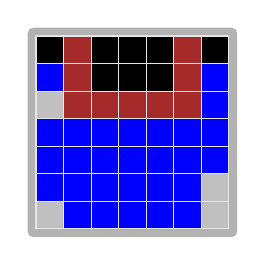
\begin{tikzpicture}
% TikZ grid exported from MARA
\def\cellsz{0.35cm}
\providecommand{\maraGridLineColor}{black!10}
\providecommand{\maraGridBorderColor}{black!30}
\providecommand{\maraGridLineWidth}{0.4pt}
\providecommand{\maraBorderLineWidth}{3pt}
\providecommand{\maraBorderRadius}{2pt}
\begin{scope}[x=\cellsz, y=\cellsz, line cap=round, line join=round]
  % Outer frame as a filled ring expanded by border line width with rounded corners
  \path[fill=\maraGridBorderColor, rounded corners=\maraBorderRadius] ([xshift=-\maraBorderLineWidth,yshift=-\maraBorderLineWidth]0,0) rectangle ([xshift=\maraBorderLineWidth,yshift=\maraBorderLineWidth]7,7);
  % Background
  \fill[black] (0,0) rectangle (7,7);
  % Filled cells
  \begin{scope}[fill={rgb,1:red,0.647;green,0.165;blue,0.165}, fill opacity=1.000]
    \fill (1,6) rectangle ++(1,1);
    \fill (5,6) rectangle ++(1,1);
    \fill (1,5) rectangle ++(1,1);
    \fill (5,5) rectangle ++(1,1);
    \fill (1,4) rectangle ++(1,1);
    \fill (2,4) rectangle ++(1,1);
    \fill (3,4) rectangle ++(1,1);
    \fill (4,4) rectangle ++(1,1);
    \fill (5,4) rectangle ++(1,1);
  \end{scope}
  \begin{scope}[fill={rgb,1:red,0.000;green,0.000;blue,1.000}, fill opacity=1.000]
    \fill (0,5) rectangle ++(1,1);
    \fill (6,5) rectangle ++(1,1);
    \fill (6,4) rectangle ++(1,1);
    \fill (0,3) rectangle ++(1,1);
    \fill (1,3) rectangle ++(1,1);
    \fill (2,3) rectangle ++(1,1);
    \fill (3,3) rectangle ++(1,1);
    \fill (4,3) rectangle ++(1,1);
    \fill (5,3) rectangle ++(1,1);
    \fill (6,3) rectangle ++(1,1);
    \fill (0,2) rectangle ++(1,1);
    \fill (1,2) rectangle ++(1,1);
    \fill (2,2) rectangle ++(1,1);
    \fill (3,2) rectangle ++(1,1);
    \fill (4,2) rectangle ++(1,1);
    \fill (5,2) rectangle ++(1,1);
    \fill (6,2) rectangle ++(1,1);
    \fill (0,1) rectangle ++(1,1);
    \fill (1,1) rectangle ++(1,1);
    \fill (2,1) rectangle ++(1,1);
    \fill (3,1) rectangle ++(1,1);
    \fill (4,1) rectangle ++(1,1);
    \fill (5,1) rectangle ++(1,1);
    \fill (1,0) rectangle ++(1,1);
    \fill (2,0) rectangle ++(1,1);
    \fill (3,0) rectangle ++(1,1);
    \fill (4,0) rectangle ++(1,1);
    \fill (5,0) rectangle ++(1,1);
  \end{scope}
  \begin{scope}[fill={rgb,1:red,0.753;green,0.753;blue,0.753}, fill opacity=1.000]
    \fill (0,4) rectangle ++(1,1);
    \fill (6,1) rectangle ++(1,1);
    \fill (0,0) rectangle ++(1,1);
    \fill (6,0) rectangle ++(1,1);
  \end{scope}
  % Grid and outline
  % Vertical lines
  \begin{scope}[draw=\maraGridLineColor, line width=\maraGridLineWidth, line cap=round]
    \draw (0,0) -- (0,7);
    \draw (1,0) -- (1,7);
    \draw (2,0) -- (2,7);
    \draw (3,0) -- (3,7);
    \draw (4,0) -- (4,7);
    \draw (5,0) -- (5,7);
    \draw (6,0) -- (6,7);
    \draw (7,0) -- (7,7);
  \end{scope}
  % Horizontal lines
  \begin{scope}[draw=\maraGridLineColor, line width=\maraGridLineWidth, line cap=round]
    \draw (0,0) -- (7,0);
    \draw (0,1) -- (7,1);
    \draw (0,2) -- (7,2);
    \draw (0,3) -- (7,3);
    \draw (0,4) -- (7,4);
    \draw (0,5) -- (7,5);
    \draw (0,6) -- (7,6);
    \draw (0,7) -- (7,7);
  \end{scope}
\end{scope}
\end{tikzpicture}
\ActionSequence{\ActionItem{noop x1}}
\medskip
% Step 50: noop x1
\smallskip
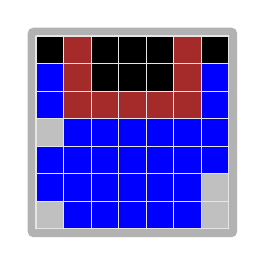
\begin{tikzpicture}
% TikZ grid exported from MARA
\def\cellsz{0.35cm}
\providecommand{\maraGridLineColor}{black!10}
\providecommand{\maraGridBorderColor}{black!30}
\providecommand{\maraGridLineWidth}{0.4pt}
\providecommand{\maraBorderLineWidth}{3pt}
\providecommand{\maraBorderRadius}{2pt}
\begin{scope}[x=\cellsz, y=\cellsz, line cap=round, line join=round]
  % Outer frame as a filled ring expanded by border line width with rounded corners
  \path[fill=\maraGridBorderColor, rounded corners=\maraBorderRadius] ([xshift=-\maraBorderLineWidth,yshift=-\maraBorderLineWidth]0,0) rectangle ([xshift=\maraBorderLineWidth,yshift=\maraBorderLineWidth]7,7);
  % Background
  \fill[black] (0,0) rectangle (7,7);
  % Filled cells
  \begin{scope}[fill={rgb,1:red,0.647;green,0.165;blue,0.165}, fill opacity=1.000]
    \fill (1,6) rectangle ++(1,1);
    \fill (5,6) rectangle ++(1,1);
    \fill (1,5) rectangle ++(1,1);
    \fill (5,5) rectangle ++(1,1);
    \fill (1,4) rectangle ++(1,1);
    \fill (2,4) rectangle ++(1,1);
    \fill (3,4) rectangle ++(1,1);
    \fill (4,4) rectangle ++(1,1);
    \fill (5,4) rectangle ++(1,1);
  \end{scope}
  \begin{scope}[fill={rgb,1:red,0.000;green,0.000;blue,1.000}, fill opacity=1.000]
    \fill (0,5) rectangle ++(1,1);
    \fill (6,5) rectangle ++(1,1);
    \fill (0,4) rectangle ++(1,1);
    \fill (6,4) rectangle ++(1,1);
    \fill (1,3) rectangle ++(1,1);
    \fill (2,3) rectangle ++(1,1);
    \fill (3,3) rectangle ++(1,1);
    \fill (4,3) rectangle ++(1,1);
    \fill (5,3) rectangle ++(1,1);
    \fill (6,3) rectangle ++(1,1);
    \fill (0,2) rectangle ++(1,1);
    \fill (1,2) rectangle ++(1,1);
    \fill (2,2) rectangle ++(1,1);
    \fill (3,2) rectangle ++(1,1);
    \fill (4,2) rectangle ++(1,1);
    \fill (5,2) rectangle ++(1,1);
    \fill (6,2) rectangle ++(1,1);
    \fill (0,1) rectangle ++(1,1);
    \fill (1,1) rectangle ++(1,1);
    \fill (2,1) rectangle ++(1,1);
    \fill (3,1) rectangle ++(1,1);
    \fill (4,1) rectangle ++(1,1);
    \fill (5,1) rectangle ++(1,1);
    \fill (1,0) rectangle ++(1,1);
    \fill (2,0) rectangle ++(1,1);
    \fill (3,0) rectangle ++(1,1);
    \fill (4,0) rectangle ++(1,1);
    \fill (5,0) rectangle ++(1,1);
  \end{scope}
  \begin{scope}[fill={rgb,1:red,0.753;green,0.753;blue,0.753}, fill opacity=1.000]
    \fill (0,3) rectangle ++(1,1);
    \fill (6,1) rectangle ++(1,1);
    \fill (0,0) rectangle ++(1,1);
    \fill (6,0) rectangle ++(1,1);
  \end{scope}
  % Grid and outline
  % Vertical lines
  \begin{scope}[draw=\maraGridLineColor, line width=\maraGridLineWidth, line cap=round]
    \draw (0,0) -- (0,7);
    \draw (1,0) -- (1,7);
    \draw (2,0) -- (2,7);
    \draw (3,0) -- (3,7);
    \draw (4,0) -- (4,7);
    \draw (5,0) -- (5,7);
    \draw (6,0) -- (6,7);
    \draw (7,0) -- (7,7);
  \end{scope}
  % Horizontal lines
  \begin{scope}[draw=\maraGridLineColor, line width=\maraGridLineWidth, line cap=round]
    \draw (0,0) -- (7,0);
    \draw (0,1) -- (7,1);
    \draw (0,2) -- (7,2);
    \draw (0,3) -- (7,3);
    \draw (0,4) -- (7,4);
    \draw (0,5) -- (7,5);
    \draw (0,6) -- (7,6);
    \draw (0,7) -- (7,7);
  \end{scope}
\end{scope}
\end{tikzpicture}
\ActionSequence{\ActionItem{noop x1}}
\medskip
% Step 51: noop x1
\smallskip
\begin{tikzpicture}
% TikZ grid exported from MARA
\def\cellsz{0.35cm}
\providecommand{\maraGridLineColor}{black!10}
\providecommand{\maraGridBorderColor}{black!30}
\providecommand{\maraGridLineWidth}{0.4pt}
\providecommand{\maraBorderLineWidth}{3pt}
\providecommand{\maraBorderRadius}{2pt}
\begin{scope}[x=\cellsz, y=\cellsz, line cap=round, line join=round]
  % Outer frame as a filled ring expanded by border line width with rounded corners
  \path[fill=\maraGridBorderColor, rounded corners=\maraBorderRadius] ([xshift=-\maraBorderLineWidth,yshift=-\maraBorderLineWidth]0,0) rectangle ([xshift=\maraBorderLineWidth,yshift=\maraBorderLineWidth]7,7);
  % Background
  \fill[black] (0,0) rectangle (7,7);
  % Filled cells
  \begin{scope}[fill={rgb,1:red,0.647;green,0.165;blue,0.165}, fill opacity=1.000]
    \fill (1,6) rectangle ++(1,1);
    \fill (5,6) rectangle ++(1,1);
    \fill (1,5) rectangle ++(1,1);
    \fill (5,5) rectangle ++(1,1);
    \fill (1,4) rectangle ++(1,1);
    \fill (2,4) rectangle ++(1,1);
    \fill (3,4) rectangle ++(1,1);
    \fill (4,4) rectangle ++(1,1);
    \fill (5,4) rectangle ++(1,1);
  \end{scope}
  \begin{scope}[fill={rgb,1:red,0.000;green,0.000;blue,1.000}, fill opacity=1.000]
    \fill (0,5) rectangle ++(1,1);
    \fill (6,5) rectangle ++(1,1);
    \fill (0,4) rectangle ++(1,1);
    \fill (6,4) rectangle ++(1,1);
    \fill (0,3) rectangle ++(1,1);
    \fill (1,3) rectangle ++(1,1);
    \fill (2,3) rectangle ++(1,1);
    \fill (3,3) rectangle ++(1,1);
    \fill (4,3) rectangle ++(1,1);
    \fill (5,3) rectangle ++(1,1);
    \fill (6,3) rectangle ++(1,1);
    \fill (1,2) rectangle ++(1,1);
    \fill (2,2) rectangle ++(1,1);
    \fill (3,2) rectangle ++(1,1);
    \fill (4,2) rectangle ++(1,1);
    \fill (5,2) rectangle ++(1,1);
    \fill (6,2) rectangle ++(1,1);
    \fill (0,1) rectangle ++(1,1);
    \fill (1,1) rectangle ++(1,1);
    \fill (2,1) rectangle ++(1,1);
    \fill (3,1) rectangle ++(1,1);
    \fill (4,1) rectangle ++(1,1);
    \fill (5,1) rectangle ++(1,1);
    \fill (1,0) rectangle ++(1,1);
    \fill (2,0) rectangle ++(1,1);
    \fill (3,0) rectangle ++(1,1);
    \fill (4,0) rectangle ++(1,1);
    \fill (5,0) rectangle ++(1,1);
  \end{scope}
  \begin{scope}[fill={rgb,1:red,0.753;green,0.753;blue,0.753}, fill opacity=1.000]
    \fill (0,2) rectangle ++(1,1);
    \fill (6,1) rectangle ++(1,1);
    \fill (0,0) rectangle ++(1,1);
    \fill (6,0) rectangle ++(1,1);
  \end{scope}
  % Grid and outline
  % Vertical lines
  \begin{scope}[draw=\maraGridLineColor, line width=\maraGridLineWidth, line cap=round]
    \draw (0,0) -- (0,7);
    \draw (1,0) -- (1,7);
    \draw (2,0) -- (2,7);
    \draw (3,0) -- (3,7);
    \draw (4,0) -- (4,7);
    \draw (5,0) -- (5,7);
    \draw (6,0) -- (6,7);
    \draw (7,0) -- (7,7);
  \end{scope}
  % Horizontal lines
  \begin{scope}[draw=\maraGridLineColor, line width=\maraGridLineWidth, line cap=round]
    \draw (0,0) -- (7,0);
    \draw (0,1) -- (7,1);
    \draw (0,2) -- (7,2);
    \draw (0,3) -- (7,3);
    \draw (0,4) -- (7,4);
    \draw (0,5) -- (7,5);
    \draw (0,6) -- (7,6);
    \draw (0,7) -- (7,7);
  \end{scope}
\end{scope}
\end{tikzpicture}
\ActionSequence{\ActionItem{noop x1}}
\medskip
% Step 52: noop x3
\smallskip
\begin{tikzpicture}
% TikZ grid exported from MARA
\def\cellsz{0.35cm}
\providecommand{\maraGridLineColor}{black!10}
\providecommand{\maraGridBorderColor}{black!30}
\providecommand{\maraGridLineWidth}{0.4pt}
\providecommand{\maraBorderLineWidth}{3pt}
\providecommand{\maraBorderRadius}{2pt}
\begin{scope}[x=\cellsz, y=\cellsz, line cap=round, line join=round]
  % Outer frame as a filled ring expanded by border line width with rounded corners
  \path[fill=\maraGridBorderColor, rounded corners=\maraBorderRadius] ([xshift=-\maraBorderLineWidth,yshift=-\maraBorderLineWidth]0,0) rectangle ([xshift=\maraBorderLineWidth,yshift=\maraBorderLineWidth]7,7);
  % Background
  \fill[black] (0,0) rectangle (7,7);
  % Filled cells
  \begin{scope}[fill={rgb,1:red,0.647;green,0.165;blue,0.165}, fill opacity=1.000]
    \fill (1,6) rectangle ++(1,1);
    \fill (5,6) rectangle ++(1,1);
    \fill (1,5) rectangle ++(1,1);
    \fill (5,5) rectangle ++(1,1);
    \fill (1,4) rectangle ++(1,1);
    \fill (2,4) rectangle ++(1,1);
    \fill (3,4) rectangle ++(1,1);
    \fill (4,4) rectangle ++(1,1);
    \fill (5,4) rectangle ++(1,1);
  \end{scope}
  \begin{scope}[fill={rgb,1:red,0.000;green,0.000;blue,1.000}, fill opacity=1.000]
    \fill (0,5) rectangle ++(1,1);
    \fill (6,5) rectangle ++(1,1);
    \fill (0,4) rectangle ++(1,1);
    \fill (6,4) rectangle ++(1,1);
    \fill (0,3) rectangle ++(1,1);
    \fill (1,3) rectangle ++(1,1);
    \fill (2,3) rectangle ++(1,1);
    \fill (3,3) rectangle ++(1,1);
    \fill (4,3) rectangle ++(1,1);
    \fill (5,3) rectangle ++(1,1);
    \fill (6,3) rectangle ++(1,1);
    \fill (0,2) rectangle ++(1,1);
    \fill (1,2) rectangle ++(1,1);
    \fill (2,2) rectangle ++(1,1);
    \fill (3,2) rectangle ++(1,1);
    \fill (4,2) rectangle ++(1,1);
    \fill (5,2) rectangle ++(1,1);
    \fill (6,2) rectangle ++(1,1);
    \fill (1,1) rectangle ++(1,1);
    \fill (2,1) rectangle ++(1,1);
    \fill (3,1) rectangle ++(1,1);
    \fill (4,1) rectangle ++(1,1);
    \fill (5,1) rectangle ++(1,1);
    \fill (1,0) rectangle ++(1,1);
    \fill (2,0) rectangle ++(1,1);
    \fill (3,0) rectangle ++(1,1);
    \fill (4,0) rectangle ++(1,1);
    \fill (5,0) rectangle ++(1,1);
  \end{scope}
  \begin{scope}[fill={rgb,1:red,0.753;green,0.753;blue,0.753}, fill opacity=1.000]
    \fill (0,1) rectangle ++(1,1);
    \fill (6,1) rectangle ++(1,1);
    \fill (0,0) rectangle ++(1,1);
    \fill (6,0) rectangle ++(1,1);
  \end{scope}
  % Grid and outline
  % Vertical lines
  \begin{scope}[draw=\maraGridLineColor, line width=\maraGridLineWidth, line cap=round]
    \draw (0,0) -- (0,7);
    \draw (1,0) -- (1,7);
    \draw (2,0) -- (2,7);
    \draw (3,0) -- (3,7);
    \draw (4,0) -- (4,7);
    \draw (5,0) -- (5,7);
    \draw (6,0) -- (6,7);
    \draw (7,0) -- (7,7);
  \end{scope}
  % Horizontal lines
  \begin{scope}[draw=\maraGridLineColor, line width=\maraGridLineWidth, line cap=round]
    \draw (0,0) -- (7,0);
    \draw (0,1) -- (7,1);
    \draw (0,2) -- (7,2);
    \draw (0,3) -- (7,3);
    \draw (0,4) -- (7,4);
    \draw (0,5) -- (7,5);
    \draw (0,6) -- (7,6);
    \draw (0,7) -- (7,7);
  \end{scope}
\end{scope}
\end{tikzpicture}
\ActionSequence{\ActionItem{noop x3}}
\medskip
% Step 53: click(0,0)
\smallskip
\begin{tikzpicture}
% TikZ grid exported from MARA
\def\cellsz{0.35cm}
\providecommand{\maraGridLineColor}{black!10}
\providecommand{\maraGridBorderColor}{black!30}
\providecommand{\maraGridLineWidth}{0.4pt}
\providecommand{\maraBorderLineWidth}{3pt}
\providecommand{\maraBorderRadius}{2pt}
\begin{scope}[x=\cellsz, y=\cellsz, line cap=round, line join=round]
  % Outer frame as a filled ring expanded by border line width with rounded corners
  \path[fill=\maraGridBorderColor, rounded corners=\maraBorderRadius] ([xshift=-\maraBorderLineWidth,yshift=-\maraBorderLineWidth]0,0) rectangle ([xshift=\maraBorderLineWidth,yshift=\maraBorderLineWidth]7,7);
  % Background
  \fill[black] (0,0) rectangle (7,7);
  % Filled cells
  \begin{scope}[fill={rgb,1:red,0.753;green,0.753;blue,0.753}, fill opacity=1.000]
    \fill (0,6) rectangle ++(1,1);
    \fill (0,1) rectangle ++(1,1);
    \fill (6,1) rectangle ++(1,1);
    \fill (0,0) rectangle ++(1,1);
    \fill (6,0) rectangle ++(1,1);
  \end{scope}
  \begin{scope}[fill={rgb,1:red,0.647;green,0.165;blue,0.165}, fill opacity=1.000]
    \fill (1,6) rectangle ++(1,1);
    \fill (5,6) rectangle ++(1,1);
    \fill (1,5) rectangle ++(1,1);
    \fill (5,5) rectangle ++(1,1);
    \fill (1,4) rectangle ++(1,1);
    \fill (2,4) rectangle ++(1,1);
    \fill (3,4) rectangle ++(1,1);
    \fill (4,4) rectangle ++(1,1);
    \fill (5,4) rectangle ++(1,1);
  \end{scope}
  \begin{scope}[fill={rgb,1:red,0.000;green,0.000;blue,1.000}, fill opacity=1.000]
    \fill (0,5) rectangle ++(1,1);
    \fill (6,5) rectangle ++(1,1);
    \fill (0,4) rectangle ++(1,1);
    \fill (6,4) rectangle ++(1,1);
    \fill (0,3) rectangle ++(1,1);
    \fill (1,3) rectangle ++(1,1);
    \fill (2,3) rectangle ++(1,1);
    \fill (3,3) rectangle ++(1,1);
    \fill (4,3) rectangle ++(1,1);
    \fill (5,3) rectangle ++(1,1);
    \fill (6,3) rectangle ++(1,1);
    \fill (0,2) rectangle ++(1,1);
    \fill (1,2) rectangle ++(1,1);
    \fill (2,2) rectangle ++(1,1);
    \fill (3,2) rectangle ++(1,1);
    \fill (4,2) rectangle ++(1,1);
    \fill (5,2) rectangle ++(1,1);
    \fill (6,2) rectangle ++(1,1);
    \fill (1,1) rectangle ++(1,1);
    \fill (2,1) rectangle ++(1,1);
    \fill (3,1) rectangle ++(1,1);
    \fill (4,1) rectangle ++(1,1);
    \fill (5,1) rectangle ++(1,1);
    \fill (1,0) rectangle ++(1,1);
    \fill (2,0) rectangle ++(1,1);
    \fill (3,0) rectangle ++(1,1);
    \fill (4,0) rectangle ++(1,1);
    \fill (5,0) rectangle ++(1,1);
  \end{scope}
  % Grid and outline
  % Vertical lines
  \begin{scope}[draw=\maraGridLineColor, line width=\maraGridLineWidth, line cap=round]
    \draw (0,0) -- (0,7);
    \draw (1,0) -- (1,7);
    \draw (2,0) -- (2,7);
    \draw (3,0) -- (3,7);
    \draw (4,0) -- (4,7);
    \draw (5,0) -- (5,7);
    \draw (6,0) -- (6,7);
    \draw (7,0) -- (7,7);
  \end{scope}
  % Horizontal lines
  \begin{scope}[draw=\maraGridLineColor, line width=\maraGridLineWidth, line cap=round]
    \draw (0,0) -- (7,0);
    \draw (0,1) -- (7,1);
    \draw (0,2) -- (7,2);
    \draw (0,3) -- (7,3);
    \draw (0,4) -- (7,4);
    \draw (0,5) -- (7,5);
    \draw (0,6) -- (7,6);
    \draw (0,7) -- (7,7);
  \end{scope}
\end{scope}
\end{tikzpicture}
\ActionSequence{\ActionItem{click(0,0)}}
\medskip
% Step 54: noop x1
\smallskip
\begin{tikzpicture}
% TikZ grid exported from MARA
\def\cellsz{0.35cm}
\providecommand{\maraGridLineColor}{black!10}
\providecommand{\maraGridBorderColor}{black!30}
\providecommand{\maraGridLineWidth}{0.4pt}
\providecommand{\maraBorderLineWidth}{3pt}
\providecommand{\maraBorderRadius}{2pt}
\begin{scope}[x=\cellsz, y=\cellsz, line cap=round, line join=round]
  % Outer frame as a filled ring expanded by border line width with rounded corners
  \path[fill=\maraGridBorderColor, rounded corners=\maraBorderRadius] ([xshift=-\maraBorderLineWidth,yshift=-\maraBorderLineWidth]0,0) rectangle ([xshift=\maraBorderLineWidth,yshift=\maraBorderLineWidth]7,7);
  % Background
  \fill[black] (0,0) rectangle (7,7);
  % Filled cells
  \begin{scope}[fill={rgb,1:red,0.000;green,0.000;blue,1.000}, fill opacity=1.000]
    \fill (0,6) rectangle ++(1,1);
    \fill (6,5) rectangle ++(1,1);
    \fill (0,4) rectangle ++(1,1);
    \fill (6,4) rectangle ++(1,1);
    \fill (0,3) rectangle ++(1,1);
    \fill (1,3) rectangle ++(1,1);
    \fill (2,3) rectangle ++(1,1);
    \fill (3,3) rectangle ++(1,1);
    \fill (4,3) rectangle ++(1,1);
    \fill (5,3) rectangle ++(1,1);
    \fill (6,3) rectangle ++(1,1);
    \fill (0,2) rectangle ++(1,1);
    \fill (1,2) rectangle ++(1,1);
    \fill (2,2) rectangle ++(1,1);
    \fill (3,2) rectangle ++(1,1);
    \fill (4,2) rectangle ++(1,1);
    \fill (5,2) rectangle ++(1,1);
    \fill (6,2) rectangle ++(1,1);
    \fill (1,1) rectangle ++(1,1);
    \fill (2,1) rectangle ++(1,1);
    \fill (3,1) rectangle ++(1,1);
    \fill (4,1) rectangle ++(1,1);
    \fill (5,1) rectangle ++(1,1);
    \fill (1,0) rectangle ++(1,1);
    \fill (2,0) rectangle ++(1,1);
    \fill (3,0) rectangle ++(1,1);
    \fill (4,0) rectangle ++(1,1);
    \fill (5,0) rectangle ++(1,1);
  \end{scope}
  \begin{scope}[fill={rgb,1:red,0.647;green,0.165;blue,0.165}, fill opacity=1.000]
    \fill (1,6) rectangle ++(1,1);
    \fill (5,6) rectangle ++(1,1);
    \fill (1,5) rectangle ++(1,1);
    \fill (5,5) rectangle ++(1,1);
    \fill (1,4) rectangle ++(1,1);
    \fill (2,4) rectangle ++(1,1);
    \fill (3,4) rectangle ++(1,1);
    \fill (4,4) rectangle ++(1,1);
    \fill (5,4) rectangle ++(1,1);
  \end{scope}
  \begin{scope}[fill={rgb,1:red,0.753;green,0.753;blue,0.753}, fill opacity=1.000]
    \fill (0,5) rectangle ++(1,1);
    \fill (0,1) rectangle ++(1,1);
    \fill (6,1) rectangle ++(1,1);
    \fill (0,0) rectangle ++(1,1);
    \fill (6,0) rectangle ++(1,1);
  \end{scope}
  % Grid and outline
  % Vertical lines
  \begin{scope}[draw=\maraGridLineColor, line width=\maraGridLineWidth, line cap=round]
    \draw (0,0) -- (0,7);
    \draw (1,0) -- (1,7);
    \draw (2,0) -- (2,7);
    \draw (3,0) -- (3,7);
    \draw (4,0) -- (4,7);
    \draw (5,0) -- (5,7);
    \draw (6,0) -- (6,7);
    \draw (7,0) -- (7,7);
  \end{scope}
  % Horizontal lines
  \begin{scope}[draw=\maraGridLineColor, line width=\maraGridLineWidth, line cap=round]
    \draw (0,0) -- (7,0);
    \draw (0,1) -- (7,1);
    \draw (0,2) -- (7,2);
    \draw (0,3) -- (7,3);
    \draw (0,4) -- (7,4);
    \draw (0,5) -- (7,5);
    \draw (0,6) -- (7,6);
    \draw (0,7) -- (7,7);
  \end{scope}
\end{scope}
\end{tikzpicture}
\ActionSequence{\ActionItem{noop x1}}
\medskip
% Step 55: noop x1
\smallskip
\begin{tikzpicture}
% TikZ grid exported from MARA
\def\cellsz{0.35cm}
\providecommand{\maraGridLineColor}{black!10}
\providecommand{\maraGridBorderColor}{black!30}
\providecommand{\maraGridLineWidth}{0.4pt}
\providecommand{\maraBorderLineWidth}{3pt}
\providecommand{\maraBorderRadius}{2pt}
\begin{scope}[x=\cellsz, y=\cellsz, line cap=round, line join=round]
  % Outer frame as a filled ring expanded by border line width with rounded corners
  \path[fill=\maraGridBorderColor, rounded corners=\maraBorderRadius] ([xshift=-\maraBorderLineWidth,yshift=-\maraBorderLineWidth]0,0) rectangle ([xshift=\maraBorderLineWidth,yshift=\maraBorderLineWidth]7,7);
  % Background
  \fill[black] (0,0) rectangle (7,7);
  % Filled cells
  \begin{scope}[fill={rgb,1:red,0.000;green,0.000;blue,1.000}, fill opacity=1.000]
    \fill (0,6) rectangle ++(1,1);
    \fill (0,5) rectangle ++(1,1);
    \fill (6,5) rectangle ++(1,1);
    \fill (6,4) rectangle ++(1,1);
    \fill (0,3) rectangle ++(1,1);
    \fill (1,3) rectangle ++(1,1);
    \fill (2,3) rectangle ++(1,1);
    \fill (3,3) rectangle ++(1,1);
    \fill (4,3) rectangle ++(1,1);
    \fill (5,3) rectangle ++(1,1);
    \fill (6,3) rectangle ++(1,1);
    \fill (0,2) rectangle ++(1,1);
    \fill (1,2) rectangle ++(1,1);
    \fill (2,2) rectangle ++(1,1);
    \fill (3,2) rectangle ++(1,1);
    \fill (4,2) rectangle ++(1,1);
    \fill (5,2) rectangle ++(1,1);
    \fill (6,2) rectangle ++(1,1);
    \fill (1,1) rectangle ++(1,1);
    \fill (2,1) rectangle ++(1,1);
    \fill (3,1) rectangle ++(1,1);
    \fill (4,1) rectangle ++(1,1);
    \fill (5,1) rectangle ++(1,1);
    \fill (1,0) rectangle ++(1,1);
    \fill (2,0) rectangle ++(1,1);
    \fill (3,0) rectangle ++(1,1);
    \fill (4,0) rectangle ++(1,1);
    \fill (5,0) rectangle ++(1,1);
  \end{scope}
  \begin{scope}[fill={rgb,1:red,0.647;green,0.165;blue,0.165}, fill opacity=1.000]
    \fill (1,6) rectangle ++(1,1);
    \fill (5,6) rectangle ++(1,1);
    \fill (1,5) rectangle ++(1,1);
    \fill (5,5) rectangle ++(1,1);
    \fill (1,4) rectangle ++(1,1);
    \fill (2,4) rectangle ++(1,1);
    \fill (3,4) rectangle ++(1,1);
    \fill (4,4) rectangle ++(1,1);
    \fill (5,4) rectangle ++(1,1);
  \end{scope}
  \begin{scope}[fill={rgb,1:red,0.753;green,0.753;blue,0.753}, fill opacity=1.000]
    \fill (0,4) rectangle ++(1,1);
    \fill (0,1) rectangle ++(1,1);
    \fill (6,1) rectangle ++(1,1);
    \fill (0,0) rectangle ++(1,1);
    \fill (6,0) rectangle ++(1,1);
  \end{scope}
  % Grid and outline
  % Vertical lines
  \begin{scope}[draw=\maraGridLineColor, line width=\maraGridLineWidth, line cap=round]
    \draw (0,0) -- (0,7);
    \draw (1,0) -- (1,7);
    \draw (2,0) -- (2,7);
    \draw (3,0) -- (3,7);
    \draw (4,0) -- (4,7);
    \draw (5,0) -- (5,7);
    \draw (6,0) -- (6,7);
    \draw (7,0) -- (7,7);
  \end{scope}
  % Horizontal lines
  \begin{scope}[draw=\maraGridLineColor, line width=\maraGridLineWidth, line cap=round]
    \draw (0,0) -- (7,0);
    \draw (0,1) -- (7,1);
    \draw (0,2) -- (7,2);
    \draw (0,3) -- (7,3);
    \draw (0,4) -- (7,4);
    \draw (0,5) -- (7,5);
    \draw (0,6) -- (7,6);
    \draw (0,7) -- (7,7);
  \end{scope}
\end{scope}
\end{tikzpicture}
\ActionSequence{\ActionItem{noop x1}}
\medskip
% Step 56: noop x1
\smallskip
\begin{tikzpicture}
% TikZ grid exported from MARA
\def\cellsz{0.35cm}
\providecommand{\maraGridLineColor}{black!10}
\providecommand{\maraGridBorderColor}{black!30}
\providecommand{\maraGridLineWidth}{0.4pt}
\providecommand{\maraBorderLineWidth}{3pt}
\providecommand{\maraBorderRadius}{2pt}
\begin{scope}[x=\cellsz, y=\cellsz, line cap=round, line join=round]
  % Outer frame as a filled ring expanded by border line width with rounded corners
  \path[fill=\maraGridBorderColor, rounded corners=\maraBorderRadius] ([xshift=-\maraBorderLineWidth,yshift=-\maraBorderLineWidth]0,0) rectangle ([xshift=\maraBorderLineWidth,yshift=\maraBorderLineWidth]7,7);
  % Background
  \fill[black] (0,0) rectangle (7,7);
  % Filled cells
  \begin{scope}[fill={rgb,1:red,0.000;green,0.000;blue,1.000}, fill opacity=1.000]
    \fill (0,6) rectangle ++(1,1);
    \fill (0,5) rectangle ++(1,1);
    \fill (6,5) rectangle ++(1,1);
    \fill (0,4) rectangle ++(1,1);
    \fill (6,4) rectangle ++(1,1);
    \fill (1,3) rectangle ++(1,1);
    \fill (2,3) rectangle ++(1,1);
    \fill (3,3) rectangle ++(1,1);
    \fill (4,3) rectangle ++(1,1);
    \fill (5,3) rectangle ++(1,1);
    \fill (6,3) rectangle ++(1,1);
    \fill (0,2) rectangle ++(1,1);
    \fill (1,2) rectangle ++(1,1);
    \fill (2,2) rectangle ++(1,1);
    \fill (3,2) rectangle ++(1,1);
    \fill (4,2) rectangle ++(1,1);
    \fill (5,2) rectangle ++(1,1);
    \fill (6,2) rectangle ++(1,1);
    \fill (1,1) rectangle ++(1,1);
    \fill (2,1) rectangle ++(1,1);
    \fill (3,1) rectangle ++(1,1);
    \fill (4,1) rectangle ++(1,1);
    \fill (5,1) rectangle ++(1,1);
    \fill (1,0) rectangle ++(1,1);
    \fill (2,0) rectangle ++(1,1);
    \fill (3,0) rectangle ++(1,1);
    \fill (4,0) rectangle ++(1,1);
    \fill (5,0) rectangle ++(1,1);
  \end{scope}
  \begin{scope}[fill={rgb,1:red,0.647;green,0.165;blue,0.165}, fill opacity=1.000]
    \fill (1,6) rectangle ++(1,1);
    \fill (5,6) rectangle ++(1,1);
    \fill (1,5) rectangle ++(1,1);
    \fill (5,5) rectangle ++(1,1);
    \fill (1,4) rectangle ++(1,1);
    \fill (2,4) rectangle ++(1,1);
    \fill (3,4) rectangle ++(1,1);
    \fill (4,4) rectangle ++(1,1);
    \fill (5,4) rectangle ++(1,1);
  \end{scope}
  \begin{scope}[fill={rgb,1:red,0.753;green,0.753;blue,0.753}, fill opacity=1.000]
    \fill (0,3) rectangle ++(1,1);
    \fill (0,1) rectangle ++(1,1);
    \fill (6,1) rectangle ++(1,1);
    \fill (0,0) rectangle ++(1,1);
    \fill (6,0) rectangle ++(1,1);
  \end{scope}
  % Grid and outline
  % Vertical lines
  \begin{scope}[draw=\maraGridLineColor, line width=\maraGridLineWidth, line cap=round]
    \draw (0,0) -- (0,7);
    \draw (1,0) -- (1,7);
    \draw (2,0) -- (2,7);
    \draw (3,0) -- (3,7);
    \draw (4,0) -- (4,7);
    \draw (5,0) -- (5,7);
    \draw (6,0) -- (6,7);
    \draw (7,0) -- (7,7);
  \end{scope}
  % Horizontal lines
  \begin{scope}[draw=\maraGridLineColor, line width=\maraGridLineWidth, line cap=round]
    \draw (0,0) -- (7,0);
    \draw (0,1) -- (7,1);
    \draw (0,2) -- (7,2);
    \draw (0,3) -- (7,3);
    \draw (0,4) -- (7,4);
    \draw (0,5) -- (7,5);
    \draw (0,6) -- (7,6);
    \draw (0,7) -- (7,7);
  \end{scope}
\end{scope}
\end{tikzpicture}
\ActionSequence{\ActionItem{noop x1}}
\medskip
% Step 57: noop x4
\smallskip
\begin{tikzpicture}
% TikZ grid exported from MARA
\def\cellsz{0.35cm}
\providecommand{\maraGridLineColor}{black!10}
\providecommand{\maraGridBorderColor}{black!30}
\providecommand{\maraGridLineWidth}{0.4pt}
\providecommand{\maraBorderLineWidth}{3pt}
\providecommand{\maraBorderRadius}{2pt}
\begin{scope}[x=\cellsz, y=\cellsz, line cap=round, line join=round]
  % Outer frame as a filled ring expanded by border line width with rounded corners
  \path[fill=\maraGridBorderColor, rounded corners=\maraBorderRadius] ([xshift=-\maraBorderLineWidth,yshift=-\maraBorderLineWidth]0,0) rectangle ([xshift=\maraBorderLineWidth,yshift=\maraBorderLineWidth]7,7);
  % Background
  \fill[black] (0,0) rectangle (7,7);
  % Filled cells
  \begin{scope}[fill={rgb,1:red,0.000;green,0.000;blue,1.000}, fill opacity=1.000]
    \fill (0,6) rectangle ++(1,1);
    \fill (0,5) rectangle ++(1,1);
    \fill (6,5) rectangle ++(1,1);
    \fill (0,4) rectangle ++(1,1);
    \fill (6,4) rectangle ++(1,1);
    \fill (0,3) rectangle ++(1,1);
    \fill (1,3) rectangle ++(1,1);
    \fill (2,3) rectangle ++(1,1);
    \fill (3,3) rectangle ++(1,1);
    \fill (4,3) rectangle ++(1,1);
    \fill (5,3) rectangle ++(1,1);
    \fill (6,3) rectangle ++(1,1);
    \fill (1,2) rectangle ++(1,1);
    \fill (2,2) rectangle ++(1,1);
    \fill (3,2) rectangle ++(1,1);
    \fill (4,2) rectangle ++(1,1);
    \fill (5,2) rectangle ++(1,1);
    \fill (6,2) rectangle ++(1,1);
    \fill (1,1) rectangle ++(1,1);
    \fill (2,1) rectangle ++(1,1);
    \fill (3,1) rectangle ++(1,1);
    \fill (4,1) rectangle ++(1,1);
    \fill (5,1) rectangle ++(1,1);
    \fill (1,0) rectangle ++(1,1);
    \fill (2,0) rectangle ++(1,1);
    \fill (3,0) rectangle ++(1,1);
    \fill (4,0) rectangle ++(1,1);
    \fill (5,0) rectangle ++(1,1);
  \end{scope}
  \begin{scope}[fill={rgb,1:red,0.647;green,0.165;blue,0.165}, fill opacity=1.000]
    \fill (1,6) rectangle ++(1,1);
    \fill (5,6) rectangle ++(1,1);
    \fill (1,5) rectangle ++(1,1);
    \fill (5,5) rectangle ++(1,1);
    \fill (1,4) rectangle ++(1,1);
    \fill (2,4) rectangle ++(1,1);
    \fill (3,4) rectangle ++(1,1);
    \fill (4,4) rectangle ++(1,1);
    \fill (5,4) rectangle ++(1,1);
  \end{scope}
  \begin{scope}[fill={rgb,1:red,0.753;green,0.753;blue,0.753}, fill opacity=1.000]
    \fill (0,2) rectangle ++(1,1);
    \fill (0,1) rectangle ++(1,1);
    \fill (6,1) rectangle ++(1,1);
    \fill (0,0) rectangle ++(1,1);
    \fill (6,0) rectangle ++(1,1);
  \end{scope}
  % Grid and outline
  % Vertical lines
  \begin{scope}[draw=\maraGridLineColor, line width=\maraGridLineWidth, line cap=round]
    \draw (0,0) -- (0,7);
    \draw (1,0) -- (1,7);
    \draw (2,0) -- (2,7);
    \draw (3,0) -- (3,7);
    \draw (4,0) -- (4,7);
    \draw (5,0) -- (5,7);
    \draw (6,0) -- (6,7);
    \draw (7,0) -- (7,7);
  \end{scope}
  % Horizontal lines
  \begin{scope}[draw=\maraGridLineColor, line width=\maraGridLineWidth, line cap=round]
    \draw (0,0) -- (7,0);
    \draw (0,1) -- (7,1);
    \draw (0,2) -- (7,2);
    \draw (0,3) -- (7,3);
    \draw (0,4) -- (7,4);
    \draw (0,5) -- (7,5);
    \draw (0,6) -- (7,6);
    \draw (0,7) -- (7,7);
  \end{scope}
\end{scope}
\end{tikzpicture}
\ActionSequence{\ActionItem{noop x4}}
\medskip
% Step 58: click(2,0)
\smallskip
\begin{tikzpicture}
% TikZ grid exported from MARA
\def\cellsz{0.35cm}
\providecommand{\maraGridLineColor}{black!10}
\providecommand{\maraGridBorderColor}{black!30}
\providecommand{\maraGridLineWidth}{0.4pt}
\providecommand{\maraBorderLineWidth}{3pt}
\providecommand{\maraBorderRadius}{2pt}
\begin{scope}[x=\cellsz, y=\cellsz, line cap=round, line join=round]
  % Outer frame as a filled ring expanded by border line width with rounded corners
  \path[fill=\maraGridBorderColor, rounded corners=\maraBorderRadius] ([xshift=-\maraBorderLineWidth,yshift=-\maraBorderLineWidth]0,0) rectangle ([xshift=\maraBorderLineWidth,yshift=\maraBorderLineWidth]7,7);
  % Background
  \fill[black] (0,0) rectangle (7,7);
  % Filled cells
  \begin{scope}[fill={rgb,1:red,0.000;green,0.000;blue,1.000}, fill opacity=1.000]
    \fill (0,6) rectangle ++(1,1);
    \fill (0,5) rectangle ++(1,1);
    \fill (6,5) rectangle ++(1,1);
    \fill (0,4) rectangle ++(1,1);
    \fill (6,4) rectangle ++(1,1);
    \fill (0,3) rectangle ++(1,1);
    \fill (1,3) rectangle ++(1,1);
    \fill (2,3) rectangle ++(1,1);
    \fill (3,3) rectangle ++(1,1);
    \fill (4,3) rectangle ++(1,1);
    \fill (5,3) rectangle ++(1,1);
    \fill (6,3) rectangle ++(1,1);
    \fill (1,2) rectangle ++(1,1);
    \fill (2,2) rectangle ++(1,1);
    \fill (3,2) rectangle ++(1,1);
    \fill (4,2) rectangle ++(1,1);
    \fill (5,2) rectangle ++(1,1);
    \fill (6,2) rectangle ++(1,1);
    \fill (1,1) rectangle ++(1,1);
    \fill (2,1) rectangle ++(1,1);
    \fill (3,1) rectangle ++(1,1);
    \fill (4,1) rectangle ++(1,1);
    \fill (5,1) rectangle ++(1,1);
    \fill (1,0) rectangle ++(1,1);
    \fill (2,0) rectangle ++(1,1);
    \fill (3,0) rectangle ++(1,1);
    \fill (4,0) rectangle ++(1,1);
    \fill (5,0) rectangle ++(1,1);
  \end{scope}
  \begin{scope}[fill={rgb,1:red,0.647;green,0.165;blue,0.165}, fill opacity=1.000]
    \fill (1,6) rectangle ++(1,1);
    \fill (5,6) rectangle ++(1,1);
    \fill (1,5) rectangle ++(1,1);
    \fill (5,5) rectangle ++(1,1);
    \fill (1,4) rectangle ++(1,1);
    \fill (2,4) rectangle ++(1,1);
    \fill (3,4) rectangle ++(1,1);
    \fill (4,4) rectangle ++(1,1);
    \fill (5,4) rectangle ++(1,1);
  \end{scope}
  \begin{scope}[fill={rgb,1:red,0.753;green,0.753;blue,0.753}, fill opacity=1.000]
    \fill (2,6) rectangle ++(1,1);
    \fill (0,2) rectangle ++(1,1);
    \fill (0,1) rectangle ++(1,1);
    \fill (6,1) rectangle ++(1,1);
    \fill (0,0) rectangle ++(1,1);
    \fill (6,0) rectangle ++(1,1);
  \end{scope}
  % Grid and outline
  % Vertical lines
  \begin{scope}[draw=\maraGridLineColor, line width=\maraGridLineWidth, line cap=round]
    \draw (0,0) -- (0,7);
    \draw (1,0) -- (1,7);
    \draw (2,0) -- (2,7);
    \draw (3,0) -- (3,7);
    \draw (4,0) -- (4,7);
    \draw (5,0) -- (5,7);
    \draw (6,0) -- (6,7);
    \draw (7,0) -- (7,7);
  \end{scope}
  % Horizontal lines
  \begin{scope}[draw=\maraGridLineColor, line width=\maraGridLineWidth, line cap=round]
    \draw (0,0) -- (7,0);
    \draw (0,1) -- (7,1);
    \draw (0,2) -- (7,2);
    \draw (0,3) -- (7,3);
    \draw (0,4) -- (7,4);
    \draw (0,5) -- (7,5);
    \draw (0,6) -- (7,6);
    \draw (0,7) -- (7,7);
  \end{scope}
\end{scope}
\end{tikzpicture}
\ActionSequence{\ActionItem{click(2,0)}}
\medskip
% Step 59: noop x1
\smallskip
\begin{tikzpicture}
% TikZ grid exported from MARA
\def\cellsz{0.35cm}
\providecommand{\maraGridLineColor}{black!10}
\providecommand{\maraGridBorderColor}{black!30}
\providecommand{\maraGridLineWidth}{0.4pt}
\providecommand{\maraBorderLineWidth}{3pt}
\providecommand{\maraBorderRadius}{2pt}
\begin{scope}[x=\cellsz, y=\cellsz, line cap=round, line join=round]
  % Outer frame as a filled ring expanded by border line width with rounded corners
  \path[fill=\maraGridBorderColor, rounded corners=\maraBorderRadius] ([xshift=-\maraBorderLineWidth,yshift=-\maraBorderLineWidth]0,0) rectangle ([xshift=\maraBorderLineWidth,yshift=\maraBorderLineWidth]7,7);
  % Background
  \fill[black] (0,0) rectangle (7,7);
  % Filled cells
  \begin{scope}[fill={rgb,1:red,0.000;green,0.000;blue,1.000}, fill opacity=1.000]
    \fill (0,6) rectangle ++(1,1);
    \fill (0,5) rectangle ++(1,1);
    \fill (6,5) rectangle ++(1,1);
    \fill (0,4) rectangle ++(1,1);
    \fill (6,4) rectangle ++(1,1);
    \fill (0,3) rectangle ++(1,1);
    \fill (6,3) rectangle ++(1,1);
    \fill (1,2) rectangle ++(1,1);
    \fill (2,2) rectangle ++(1,1);
    \fill (3,2) rectangle ++(1,1);
    \fill (4,2) rectangle ++(1,1);
    \fill (5,2) rectangle ++(1,1);
    \fill (6,2) rectangle ++(1,1);
    \fill (1,1) rectangle ++(1,1);
    \fill (2,1) rectangle ++(1,1);
    \fill (3,1) rectangle ++(1,1);
    \fill (4,1) rectangle ++(1,1);
    \fill (5,1) rectangle ++(1,1);
    \fill (1,0) rectangle ++(1,1);
    \fill (2,0) rectangle ++(1,1);
    \fill (3,0) rectangle ++(1,1);
    \fill (4,0) rectangle ++(1,1);
    \fill (5,0) rectangle ++(1,1);
  \end{scope}
  \begin{scope}[fill={rgb,1:red,0.647;green,0.165;blue,0.165}, fill opacity=1.000]
    \fill (1,5) rectangle ++(1,1);
    \fill (5,5) rectangle ++(1,1);
    \fill (1,4) rectangle ++(1,1);
    \fill (5,4) rectangle ++(1,1);
    \fill (1,3) rectangle ++(1,1);
    \fill (2,3) rectangle ++(1,1);
    \fill (3,3) rectangle ++(1,1);
    \fill (4,3) rectangle ++(1,1);
    \fill (5,3) rectangle ++(1,1);
  \end{scope}
  \begin{scope}[fill={rgb,1:red,0.753;green,0.753;blue,0.753}, fill opacity=1.000]
    \fill (2,5) rectangle ++(1,1);
    \fill (0,2) rectangle ++(1,1);
    \fill (0,1) rectangle ++(1,1);
    \fill (6,1) rectangle ++(1,1);
    \fill (0,0) rectangle ++(1,1);
    \fill (6,0) rectangle ++(1,1);
  \end{scope}
  % Grid and outline
  % Vertical lines
  \begin{scope}[draw=\maraGridLineColor, line width=\maraGridLineWidth, line cap=round]
    \draw (0,0) -- (0,7);
    \draw (1,0) -- (1,7);
    \draw (2,0) -- (2,7);
    \draw (3,0) -- (3,7);
    \draw (4,0) -- (4,7);
    \draw (5,0) -- (5,7);
    \draw (6,0) -- (6,7);
    \draw (7,0) -- (7,7);
  \end{scope}
  % Horizontal lines
  \begin{scope}[draw=\maraGridLineColor, line width=\maraGridLineWidth, line cap=round]
    \draw (0,0) -- (7,0);
    \draw (0,1) -- (7,1);
    \draw (0,2) -- (7,2);
    \draw (0,3) -- (7,3);
    \draw (0,4) -- (7,4);
    \draw (0,5) -- (7,5);
    \draw (0,6) -- (7,6);
    \draw (0,7) -- (7,7);
  \end{scope}
\end{scope}
\end{tikzpicture}
\ActionSequence{\ActionItem{noop x1}}
\medskip
% Step 60: noop x1
\smallskip
\begin{tikzpicture}
% TikZ grid exported from MARA
\def\cellsz{0.35cm}
\providecommand{\maraGridLineColor}{black!10}
\providecommand{\maraGridBorderColor}{black!30}
\providecommand{\maraGridLineWidth}{0.4pt}
\providecommand{\maraBorderLineWidth}{3pt}
\providecommand{\maraBorderRadius}{2pt}
\begin{scope}[x=\cellsz, y=\cellsz, line cap=round, line join=round]
  % Outer frame as a filled ring expanded by border line width with rounded corners
  \path[fill=\maraGridBorderColor, rounded corners=\maraBorderRadius] ([xshift=-\maraBorderLineWidth,yshift=-\maraBorderLineWidth]0,0) rectangle ([xshift=\maraBorderLineWidth,yshift=\maraBorderLineWidth]7,7);
  % Background
  \fill[black] (0,0) rectangle (7,7);
  % Filled cells
  \begin{scope}[fill={rgb,1:red,0.000;green,0.000;blue,1.000}, fill opacity=1.000]
    \fill (1,6) rectangle ++(1,1);
    \fill (0,5) rectangle ++(1,1);
    \fill (6,5) rectangle ++(1,1);
    \fill (0,4) rectangle ++(1,1);
    \fill (6,4) rectangle ++(1,1);
    \fill (0,3) rectangle ++(1,1);
    \fill (6,3) rectangle ++(1,1);
    \fill (1,2) rectangle ++(1,1);
    \fill (2,2) rectangle ++(1,1);
    \fill (3,2) rectangle ++(1,1);
    \fill (4,2) rectangle ++(1,1);
    \fill (5,2) rectangle ++(1,1);
    \fill (6,2) rectangle ++(1,1);
    \fill (1,1) rectangle ++(1,1);
    \fill (2,1) rectangle ++(1,1);
    \fill (3,1) rectangle ++(1,1);
    \fill (4,1) rectangle ++(1,1);
    \fill (5,1) rectangle ++(1,1);
    \fill (1,0) rectangle ++(1,1);
    \fill (2,0) rectangle ++(1,1);
    \fill (3,0) rectangle ++(1,1);
    \fill (4,0) rectangle ++(1,1);
    \fill (5,0) rectangle ++(1,1);
  \end{scope}
  \begin{scope}[fill={rgb,1:red,0.647;green,0.165;blue,0.165}, fill opacity=1.000]
    \fill (1,5) rectangle ++(1,1);
    \fill (5,5) rectangle ++(1,1);
    \fill (1,4) rectangle ++(1,1);
    \fill (5,4) rectangle ++(1,1);
    \fill (1,3) rectangle ++(1,1);
    \fill (2,3) rectangle ++(1,1);
    \fill (3,3) rectangle ++(1,1);
    \fill (4,3) rectangle ++(1,1);
    \fill (5,3) rectangle ++(1,1);
  \end{scope}
  \begin{scope}[fill={rgb,1:red,0.753;green,0.753;blue,0.753}, fill opacity=1.000]
    \fill (2,4) rectangle ++(1,1);
    \fill (0,2) rectangle ++(1,1);
    \fill (0,1) rectangle ++(1,1);
    \fill (6,1) rectangle ++(1,1);
    \fill (0,0) rectangle ++(1,1);
    \fill (6,0) rectangle ++(1,1);
  \end{scope}
  % Grid and outline
  % Vertical lines
  \begin{scope}[draw=\maraGridLineColor, line width=\maraGridLineWidth, line cap=round]
    \draw (0,0) -- (0,7);
    \draw (1,0) -- (1,7);
    \draw (2,0) -- (2,7);
    \draw (3,0) -- (3,7);
    \draw (4,0) -- (4,7);
    \draw (5,0) -- (5,7);
    \draw (6,0) -- (6,7);
    \draw (7,0) -- (7,7);
  \end{scope}
  % Horizontal lines
  \begin{scope}[draw=\maraGridLineColor, line width=\maraGridLineWidth, line cap=round]
    \draw (0,0) -- (7,0);
    \draw (0,1) -- (7,1);
    \draw (0,2) -- (7,2);
    \draw (0,3) -- (7,3);
    \draw (0,4) -- (7,4);
    \draw (0,5) -- (7,5);
    \draw (0,6) -- (7,6);
    \draw (0,7) -- (7,7);
  \end{scope}
\end{scope}
\end{tikzpicture}
\ActionSequence{\ActionItem{noop x1}}
\medskip
% Step 61: noop x1
\smallskip
\begin{tikzpicture}
% TikZ grid exported from MARA
\def\cellsz{0.35cm}
\providecommand{\maraGridLineColor}{black!10}
\providecommand{\maraGridBorderColor}{black!30}
\providecommand{\maraGridLineWidth}{0.4pt}
\providecommand{\maraBorderLineWidth}{3pt}
\providecommand{\maraBorderRadius}{2pt}
\begin{scope}[x=\cellsz, y=\cellsz, line cap=round, line join=round]
  % Outer frame as a filled ring expanded by border line width with rounded corners
  \path[fill=\maraGridBorderColor, rounded corners=\maraBorderRadius] ([xshift=-\maraBorderLineWidth,yshift=-\maraBorderLineWidth]0,0) rectangle ([xshift=\maraBorderLineWidth,yshift=\maraBorderLineWidth]7,7);
  % Background
  \fill[black] (0,0) rectangle (7,7);
  % Filled cells
  \begin{scope}[fill={rgb,1:red,0.000;green,0.000;blue,1.000}, fill opacity=1.000]
    \fill (2,6) rectangle ++(1,1);
    \fill (0,5) rectangle ++(1,1);
    \fill (6,5) rectangle ++(1,1);
    \fill (0,4) rectangle ++(1,1);
    \fill (6,4) rectangle ++(1,1);
    \fill (0,3) rectangle ++(1,1);
    \fill (6,3) rectangle ++(1,1);
    \fill (1,2) rectangle ++(1,1);
    \fill (2,2) rectangle ++(1,1);
    \fill (3,2) rectangle ++(1,1);
    \fill (4,2) rectangle ++(1,1);
    \fill (5,2) rectangle ++(1,1);
    \fill (6,2) rectangle ++(1,1);
    \fill (1,1) rectangle ++(1,1);
    \fill (2,1) rectangle ++(1,1);
    \fill (3,1) rectangle ++(1,1);
    \fill (4,1) rectangle ++(1,1);
    \fill (5,1) rectangle ++(1,1);
    \fill (1,0) rectangle ++(1,1);
    \fill (2,0) rectangle ++(1,1);
    \fill (3,0) rectangle ++(1,1);
    \fill (4,0) rectangle ++(1,1);
    \fill (5,0) rectangle ++(1,1);
  \end{scope}
  \begin{scope}[fill={rgb,1:red,0.647;green,0.165;blue,0.165}, fill opacity=1.000]
    \fill (1,5) rectangle ++(1,1);
    \fill (5,5) rectangle ++(1,1);
    \fill (1,4) rectangle ++(1,1);
    \fill (5,4) rectangle ++(1,1);
    \fill (1,3) rectangle ++(1,1);
    \fill (2,3) rectangle ++(1,1);
    \fill (3,3) rectangle ++(1,1);
    \fill (4,3) rectangle ++(1,1);
    \fill (5,3) rectangle ++(1,1);
  \end{scope}
  \begin{scope}[fill={rgb,1:red,0.753;green,0.753;blue,0.753}, fill opacity=1.000]
    \fill (2,4) rectangle ++(1,1);
    \fill (0,2) rectangle ++(1,1);
    \fill (0,1) rectangle ++(1,1);
    \fill (6,1) rectangle ++(1,1);
    \fill (0,0) rectangle ++(1,1);
    \fill (6,0) rectangle ++(1,1);
  \end{scope}
  % Grid and outline
  % Vertical lines
  \begin{scope}[draw=\maraGridLineColor, line width=\maraGridLineWidth, line cap=round]
    \draw (0,0) -- (0,7);
    \draw (1,0) -- (1,7);
    \draw (2,0) -- (2,7);
    \draw (3,0) -- (3,7);
    \draw (4,0) -- (4,7);
    \draw (5,0) -- (5,7);
    \draw (6,0) -- (6,7);
    \draw (7,0) -- (7,7);
  \end{scope}
  % Horizontal lines
  \begin{scope}[draw=\maraGridLineColor, line width=\maraGridLineWidth, line cap=round]
    \draw (0,0) -- (7,0);
    \draw (0,1) -- (7,1);
    \draw (0,2) -- (7,2);
    \draw (0,3) -- (7,3);
    \draw (0,4) -- (7,4);
    \draw (0,5) -- (7,5);
    \draw (0,6) -- (7,6);
    \draw (0,7) -- (7,7);
  \end{scope}
\end{scope}
\end{tikzpicture}
\ActionSequence{\ActionItem{noop x1}}
\medskip
% Step 62: noop x1
\smallskip
\begin{tikzpicture}
% TikZ grid exported from MARA
\def\cellsz{0.35cm}
\providecommand{\maraGridLineColor}{black!10}
\providecommand{\maraGridBorderColor}{black!30}
\providecommand{\maraGridLineWidth}{0.4pt}
\providecommand{\maraBorderLineWidth}{3pt}
\providecommand{\maraBorderRadius}{2pt}
\begin{scope}[x=\cellsz, y=\cellsz, line cap=round, line join=round]
  % Outer frame as a filled ring expanded by border line width with rounded corners
  \path[fill=\maraGridBorderColor, rounded corners=\maraBorderRadius] ([xshift=-\maraBorderLineWidth,yshift=-\maraBorderLineWidth]0,0) rectangle ([xshift=\maraBorderLineWidth,yshift=\maraBorderLineWidth]7,7);
  % Background
  \fill[black] (0,0) rectangle (7,7);
  % Filled cells
  \begin{scope}[fill={rgb,1:red,0.000;green,0.000;blue,1.000}, fill opacity=1.000]
    \fill (0,5) rectangle ++(1,1);
    \fill (2,5) rectangle ++(1,1);
    \fill (6,5) rectangle ++(1,1);
    \fill (0,4) rectangle ++(1,1);
    \fill (6,4) rectangle ++(1,1);
    \fill (0,3) rectangle ++(1,1);
    \fill (6,3) rectangle ++(1,1);
    \fill (1,2) rectangle ++(1,1);
    \fill (2,2) rectangle ++(1,1);
    \fill (3,2) rectangle ++(1,1);
    \fill (4,2) rectangle ++(1,1);
    \fill (5,2) rectangle ++(1,1);
    \fill (6,2) rectangle ++(1,1);
    \fill (1,1) rectangle ++(1,1);
    \fill (2,1) rectangle ++(1,1);
    \fill (3,1) rectangle ++(1,1);
    \fill (4,1) rectangle ++(1,1);
    \fill (5,1) rectangle ++(1,1);
    \fill (1,0) rectangle ++(1,1);
    \fill (2,0) rectangle ++(1,1);
    \fill (3,0) rectangle ++(1,1);
    \fill (4,0) rectangle ++(1,1);
    \fill (5,0) rectangle ++(1,1);
  \end{scope}
  \begin{scope}[fill={rgb,1:red,0.647;green,0.165;blue,0.165}, fill opacity=1.000]
    \fill (1,5) rectangle ++(1,1);
    \fill (5,5) rectangle ++(1,1);
    \fill (1,4) rectangle ++(1,1);
    \fill (5,4) rectangle ++(1,1);
    \fill (1,3) rectangle ++(1,1);
    \fill (2,3) rectangle ++(1,1);
    \fill (3,3) rectangle ++(1,1);
    \fill (4,3) rectangle ++(1,1);
    \fill (5,3) rectangle ++(1,1);
  \end{scope}
  \begin{scope}[fill={rgb,1:red,0.753;green,0.753;blue,0.753}, fill opacity=1.000]
    \fill (2,4) rectangle ++(1,1);
    \fill (0,2) rectangle ++(1,1);
    \fill (0,1) rectangle ++(1,1);
    \fill (6,1) rectangle ++(1,1);
    \fill (0,0) rectangle ++(1,1);
    \fill (6,0) rectangle ++(1,1);
  \end{scope}
  % Grid and outline
  % Vertical lines
  \begin{scope}[draw=\maraGridLineColor, line width=\maraGridLineWidth, line cap=round]
    \draw (0,0) -- (0,7);
    \draw (1,0) -- (1,7);
    \draw (2,0) -- (2,7);
    \draw (3,0) -- (3,7);
    \draw (4,0) -- (4,7);
    \draw (5,0) -- (5,7);
    \draw (6,0) -- (6,7);
    \draw (7,0) -- (7,7);
  \end{scope}
  % Horizontal lines
  \begin{scope}[draw=\maraGridLineColor, line width=\maraGridLineWidth, line cap=round]
    \draw (0,0) -- (7,0);
    \draw (0,1) -- (7,1);
    \draw (0,2) -- (7,2);
    \draw (0,3) -- (7,3);
    \draw (0,4) -- (7,4);
    \draw (0,5) -- (7,5);
    \draw (0,6) -- (7,6);
    \draw (0,7) -- (7,7);
  \end{scope}
\end{scope}
\end{tikzpicture}
\ActionSequence{\ActionItem{noop x1}}
\medskip
% Step 63: noop x1
\smallskip
\begin{tikzpicture}
% TikZ grid exported from MARA
\def\cellsz{0.35cm}
\providecommand{\maraGridLineColor}{black!10}
\providecommand{\maraGridBorderColor}{black!30}
\providecommand{\maraGridLineWidth}{0.4pt}
\providecommand{\maraBorderLineWidth}{3pt}
\providecommand{\maraBorderRadius}{2pt}
\begin{scope}[x=\cellsz, y=\cellsz, line cap=round, line join=round]
  % Outer frame as a filled ring expanded by border line width with rounded corners
  \path[fill=\maraGridBorderColor, rounded corners=\maraBorderRadius] ([xshift=-\maraBorderLineWidth,yshift=-\maraBorderLineWidth]0,0) rectangle ([xshift=\maraBorderLineWidth,yshift=\maraBorderLineWidth]7,7);
  % Background
  \fill[black] (0,0) rectangle (7,7);
  % Filled cells
  \begin{scope}[fill={rgb,1:red,0.000;green,0.000;blue,1.000}, fill opacity=1.000]
    \fill (0,5) rectangle ++(1,1);
    \fill (3,5) rectangle ++(1,1);
    \fill (6,5) rectangle ++(1,1);
    \fill (0,4) rectangle ++(1,1);
    \fill (6,4) rectangle ++(1,1);
    \fill (0,3) rectangle ++(1,1);
    \fill (6,3) rectangle ++(1,1);
    \fill (1,2) rectangle ++(1,1);
    \fill (2,2) rectangle ++(1,1);
    \fill (3,2) rectangle ++(1,1);
    \fill (4,2) rectangle ++(1,1);
    \fill (5,2) rectangle ++(1,1);
    \fill (6,2) rectangle ++(1,1);
    \fill (1,1) rectangle ++(1,1);
    \fill (2,1) rectangle ++(1,1);
    \fill (3,1) rectangle ++(1,1);
    \fill (4,1) rectangle ++(1,1);
    \fill (5,1) rectangle ++(1,1);
    \fill (1,0) rectangle ++(1,1);
    \fill (2,0) rectangle ++(1,1);
    \fill (3,0) rectangle ++(1,1);
    \fill (4,0) rectangle ++(1,1);
    \fill (5,0) rectangle ++(1,1);
  \end{scope}
  \begin{scope}[fill={rgb,1:red,0.647;green,0.165;blue,0.165}, fill opacity=1.000]
    \fill (1,5) rectangle ++(1,1);
    \fill (5,5) rectangle ++(1,1);
    \fill (1,4) rectangle ++(1,1);
    \fill (5,4) rectangle ++(1,1);
    \fill (1,3) rectangle ++(1,1);
    \fill (2,3) rectangle ++(1,1);
    \fill (3,3) rectangle ++(1,1);
    \fill (4,3) rectangle ++(1,1);
    \fill (5,3) rectangle ++(1,1);
  \end{scope}
  \begin{scope}[fill={rgb,1:red,0.753;green,0.753;blue,0.753}, fill opacity=1.000]
    \fill (2,4) rectangle ++(1,1);
    \fill (0,2) rectangle ++(1,1);
    \fill (0,1) rectangle ++(1,1);
    \fill (6,1) rectangle ++(1,1);
    \fill (0,0) rectangle ++(1,1);
    \fill (6,0) rectangle ++(1,1);
  \end{scope}
  % Grid and outline
  % Vertical lines
  \begin{scope}[draw=\maraGridLineColor, line width=\maraGridLineWidth, line cap=round]
    \draw (0,0) -- (0,7);
    \draw (1,0) -- (1,7);
    \draw (2,0) -- (2,7);
    \draw (3,0) -- (3,7);
    \draw (4,0) -- (4,7);
    \draw (5,0) -- (5,7);
    \draw (6,0) -- (6,7);
    \draw (7,0) -- (7,7);
  \end{scope}
  % Horizontal lines
  \begin{scope}[draw=\maraGridLineColor, line width=\maraGridLineWidth, line cap=round]
    \draw (0,0) -- (7,0);
    \draw (0,1) -- (7,1);
    \draw (0,2) -- (7,2);
    \draw (0,3) -- (7,3);
    \draw (0,4) -- (7,4);
    \draw (0,5) -- (7,5);
    \draw (0,6) -- (7,6);
    \draw (0,7) -- (7,7);
  \end{scope}
\end{scope}
\end{tikzpicture}
\ActionSequence{\ActionItem{noop x1}}
\medskip
% Step 64: noop x11
\smallskip
\begin{tikzpicture}
% TikZ grid exported from MARA
\def\cellsz{0.35cm}
\providecommand{\maraGridLineColor}{black!10}
\providecommand{\maraGridBorderColor}{black!30}
\providecommand{\maraGridLineWidth}{0.4pt}
\providecommand{\maraBorderLineWidth}{3pt}
\providecommand{\maraBorderRadius}{2pt}
\begin{scope}[x=\cellsz, y=\cellsz, line cap=round, line join=round]
  % Outer frame as a filled ring expanded by border line width with rounded corners
  \path[fill=\maraGridBorderColor, rounded corners=\maraBorderRadius] ([xshift=-\maraBorderLineWidth,yshift=-\maraBorderLineWidth]0,0) rectangle ([xshift=\maraBorderLineWidth,yshift=\maraBorderLineWidth]7,7);
  % Background
  \fill[black] (0,0) rectangle (7,7);
  % Filled cells
  \begin{scope}[fill={rgb,1:red,0.000;green,0.000;blue,1.000}, fill opacity=1.000]
    \fill (0,5) rectangle ++(1,1);
    \fill (6,5) rectangle ++(1,1);
    \fill (0,4) rectangle ++(1,1);
    \fill (3,4) rectangle ++(1,1);
    \fill (6,4) rectangle ++(1,1);
    \fill (0,3) rectangle ++(1,1);
    \fill (6,3) rectangle ++(1,1);
    \fill (1,2) rectangle ++(1,1);
    \fill (2,2) rectangle ++(1,1);
    \fill (3,2) rectangle ++(1,1);
    \fill (4,2) rectangle ++(1,1);
    \fill (5,2) rectangle ++(1,1);
    \fill (6,2) rectangle ++(1,1);
    \fill (1,1) rectangle ++(1,1);
    \fill (2,1) rectangle ++(1,1);
    \fill (3,1) rectangle ++(1,1);
    \fill (4,1) rectangle ++(1,1);
    \fill (5,1) rectangle ++(1,1);
    \fill (1,0) rectangle ++(1,1);
    \fill (2,0) rectangle ++(1,1);
    \fill (3,0) rectangle ++(1,1);
    \fill (4,0) rectangle ++(1,1);
    \fill (5,0) rectangle ++(1,1);
  \end{scope}
  \begin{scope}[fill={rgb,1:red,0.647;green,0.165;blue,0.165}, fill opacity=1.000]
    \fill (1,5) rectangle ++(1,1);
    \fill (5,5) rectangle ++(1,1);
    \fill (1,4) rectangle ++(1,1);
    \fill (5,4) rectangle ++(1,1);
    \fill (1,3) rectangle ++(1,1);
    \fill (2,3) rectangle ++(1,1);
    \fill (3,3) rectangle ++(1,1);
    \fill (4,3) rectangle ++(1,1);
    \fill (5,3) rectangle ++(1,1);
  \end{scope}
  \begin{scope}[fill={rgb,1:red,0.753;green,0.753;blue,0.753}, fill opacity=1.000]
    \fill (2,4) rectangle ++(1,1);
    \fill (0,2) rectangle ++(1,1);
    \fill (0,1) rectangle ++(1,1);
    \fill (6,1) rectangle ++(1,1);
    \fill (0,0) rectangle ++(1,1);
    \fill (6,0) rectangle ++(1,1);
  \end{scope}
  % Grid and outline
  % Vertical lines
  \begin{scope}[draw=\maraGridLineColor, line width=\maraGridLineWidth, line cap=round]
    \draw (0,0) -- (0,7);
    \draw (1,0) -- (1,7);
    \draw (2,0) -- (2,7);
    \draw (3,0) -- (3,7);
    \draw (4,0) -- (4,7);
    \draw (5,0) -- (5,7);
    \draw (6,0) -- (6,7);
    \draw (7,0) -- (7,7);
  \end{scope}
  % Horizontal lines
  \begin{scope}[draw=\maraGridLineColor, line width=\maraGridLineWidth, line cap=round]
    \draw (0,0) -- (7,0);
    \draw (0,1) -- (7,1);
    \draw (0,2) -- (7,2);
    \draw (0,3) -- (7,3);
    \draw (0,4) -- (7,4);
    \draw (0,5) -- (7,5);
    \draw (0,6) -- (7,6);
    \draw (0,7) -- (7,7);
  \end{scope}
\end{scope}
\end{tikzpicture}
\ActionSequence{\ActionItem{noop x11}}
\medskip
% Step 65: click(4,1)
\smallskip
\begin{tikzpicture}
% TikZ grid exported from MARA
\def\cellsz{0.35cm}
\providecommand{\maraGridLineColor}{black!10}
\providecommand{\maraGridBorderColor}{black!30}
\providecommand{\maraGridLineWidth}{0.4pt}
\providecommand{\maraBorderLineWidth}{3pt}
\providecommand{\maraBorderRadius}{2pt}
\begin{scope}[x=\cellsz, y=\cellsz, line cap=round, line join=round]
  % Outer frame as a filled ring expanded by border line width with rounded corners
  \path[fill=\maraGridBorderColor, rounded corners=\maraBorderRadius] ([xshift=-\maraBorderLineWidth,yshift=-\maraBorderLineWidth]0,0) rectangle ([xshift=\maraBorderLineWidth,yshift=\maraBorderLineWidth]7,7);
  % Background
  \fill[black] (0,0) rectangle (7,7);
  % Filled cells
  \begin{scope}[fill={rgb,1:red,0.000;green,0.000;blue,1.000}, fill opacity=1.000]
    \fill (0,5) rectangle ++(1,1);
    \fill (6,5) rectangle ++(1,1);
    \fill (0,4) rectangle ++(1,1);
    \fill (3,4) rectangle ++(1,1);
    \fill (6,4) rectangle ++(1,1);
    \fill (0,3) rectangle ++(1,1);
    \fill (6,3) rectangle ++(1,1);
    \fill (1,2) rectangle ++(1,1);
    \fill (2,2) rectangle ++(1,1);
    \fill (3,2) rectangle ++(1,1);
    \fill (4,2) rectangle ++(1,1);
    \fill (5,2) rectangle ++(1,1);
    \fill (6,2) rectangle ++(1,1);
    \fill (1,1) rectangle ++(1,1);
    \fill (2,1) rectangle ++(1,1);
    \fill (3,1) rectangle ++(1,1);
    \fill (4,1) rectangle ++(1,1);
    \fill (5,1) rectangle ++(1,1);
    \fill (1,0) rectangle ++(1,1);
    \fill (2,0) rectangle ++(1,1);
    \fill (3,0) rectangle ++(1,1);
    \fill (4,0) rectangle ++(1,1);
    \fill (5,0) rectangle ++(1,1);
  \end{scope}
  \begin{scope}[fill={rgb,1:red,0.647;green,0.165;blue,0.165}, fill opacity=1.000]
    \fill (1,5) rectangle ++(1,1);
    \fill (5,5) rectangle ++(1,1);
    \fill (1,4) rectangle ++(1,1);
    \fill (5,4) rectangle ++(1,1);
    \fill (1,3) rectangle ++(1,1);
    \fill (2,3) rectangle ++(1,1);
    \fill (3,3) rectangle ++(1,1);
    \fill (4,3) rectangle ++(1,1);
    \fill (5,3) rectangle ++(1,1);
  \end{scope}
  \begin{scope}[fill={rgb,1:red,0.753;green,0.753;blue,0.753}, fill opacity=1.000]
    \fill (4,5) rectangle ++(1,1);
    \fill (2,4) rectangle ++(1,1);
    \fill (0,2) rectangle ++(1,1);
    \fill (0,1) rectangle ++(1,1);
    \fill (6,1) rectangle ++(1,1);
    \fill (0,0) rectangle ++(1,1);
    \fill (6,0) rectangle ++(1,1);
  \end{scope}
  % Grid and outline
  % Vertical lines
  \begin{scope}[draw=\maraGridLineColor, line width=\maraGridLineWidth, line cap=round]
    \draw (0,0) -- (0,7);
    \draw (1,0) -- (1,7);
    \draw (2,0) -- (2,7);
    \draw (3,0) -- (3,7);
    \draw (4,0) -- (4,7);
    \draw (5,0) -- (5,7);
    \draw (6,0) -- (6,7);
    \draw (7,0) -- (7,7);
  \end{scope}
  % Horizontal lines
  \begin{scope}[draw=\maraGridLineColor, line width=\maraGridLineWidth, line cap=round]
    \draw (0,0) -- (7,0);
    \draw (0,1) -- (7,1);
    \draw (0,2) -- (7,2);
    \draw (0,3) -- (7,3);
    \draw (0,4) -- (7,4);
    \draw (0,5) -- (7,5);
    \draw (0,6) -- (7,6);
    \draw (0,7) -- (7,7);
  \end{scope}
\end{scope}
\end{tikzpicture}
\ActionSequence{\ActionItem{click(4,1)}}
\medskip
% Step 66: noop x1
\smallskip
\begin{tikzpicture}
% TikZ grid exported from MARA
\def\cellsz{0.35cm}
\providecommand{\maraGridLineColor}{black!10}
\providecommand{\maraGridBorderColor}{black!30}
\providecommand{\maraGridLineWidth}{0.4pt}
\providecommand{\maraBorderLineWidth}{3pt}
\providecommand{\maraBorderRadius}{2pt}
\begin{scope}[x=\cellsz, y=\cellsz, line cap=round, line join=round]
  % Outer frame as a filled ring expanded by border line width with rounded corners
  \path[fill=\maraGridBorderColor, rounded corners=\maraBorderRadius] ([xshift=-\maraBorderLineWidth,yshift=-\maraBorderLineWidth]0,0) rectangle ([xshift=\maraBorderLineWidth,yshift=\maraBorderLineWidth]7,7);
  % Background
  \fill[black] (0,0) rectangle (7,7);
  % Filled cells
  \begin{scope}[fill={rgb,1:red,0.000;green,0.000;blue,1.000}, fill opacity=1.000]
    \fill (0,5) rectangle ++(1,1);
    \fill (6,5) rectangle ++(1,1);
    \fill (0,4) rectangle ++(1,1);
    \fill (2,4) rectangle ++(1,1);
    \fill (3,4) rectangle ++(1,1);
    \fill (6,4) rectangle ++(1,1);
    \fill (0,3) rectangle ++(1,1);
    \fill (3,3) rectangle ++(1,1);
    \fill (4,3) rectangle ++(1,1);
    \fill (6,3) rectangle ++(1,1);
    \fill (6,2) rectangle ++(1,1);
    \fill (1,1) rectangle ++(1,1);
    \fill (2,1) rectangle ++(1,1);
    \fill (3,1) rectangle ++(1,1);
    \fill (4,1) rectangle ++(1,1);
    \fill (5,1) rectangle ++(1,1);
    \fill (1,0) rectangle ++(1,1);
    \fill (2,0) rectangle ++(1,1);
    \fill (3,0) rectangle ++(1,1);
    \fill (4,0) rectangle ++(1,1);
    \fill (5,0) rectangle ++(1,1);
  \end{scope}
  \begin{scope}[fill={rgb,1:red,0.647;green,0.165;blue,0.165}, fill opacity=1.000]
    \fill (1,4) rectangle ++(1,1);
    \fill (5,4) rectangle ++(1,1);
    \fill (1,3) rectangle ++(1,1);
    \fill (5,3) rectangle ++(1,1);
    \fill (1,2) rectangle ++(1,1);
    \fill (2,2) rectangle ++(1,1);
    \fill (3,2) rectangle ++(1,1);
    \fill (4,2) rectangle ++(1,1);
    \fill (5,2) rectangle ++(1,1);
  \end{scope}
  \begin{scope}[fill={rgb,1:red,0.753;green,0.753;blue,0.753}, fill opacity=1.000]
    \fill (4,4) rectangle ++(1,1);
    \fill (2,3) rectangle ++(1,1);
    \fill (0,2) rectangle ++(1,1);
    \fill (0,1) rectangle ++(1,1);
    \fill (6,1) rectangle ++(1,1);
    \fill (0,0) rectangle ++(1,1);
    \fill (6,0) rectangle ++(1,1);
  \end{scope}
  % Grid and outline
  % Vertical lines
  \begin{scope}[draw=\maraGridLineColor, line width=\maraGridLineWidth, line cap=round]
    \draw (0,0) -- (0,7);
    \draw (1,0) -- (1,7);
    \draw (2,0) -- (2,7);
    \draw (3,0) -- (3,7);
    \draw (4,0) -- (4,7);
    \draw (5,0) -- (5,7);
    \draw (6,0) -- (6,7);
    \draw (7,0) -- (7,7);
  \end{scope}
  % Horizontal lines
  \begin{scope}[draw=\maraGridLineColor, line width=\maraGridLineWidth, line cap=round]
    \draw (0,0) -- (7,0);
    \draw (0,1) -- (7,1);
    \draw (0,2) -- (7,2);
    \draw (0,3) -- (7,3);
    \draw (0,4) -- (7,4);
    \draw (0,5) -- (7,5);
    \draw (0,6) -- (7,6);
    \draw (0,7) -- (7,7);
  \end{scope}
\end{scope}
\end{tikzpicture}
\ActionSequence{\ActionItem{noop x1}}
\medskip
% Step 67: noop x13
\smallskip
\begin{tikzpicture}
% TikZ grid exported from MARA
\def\cellsz{0.35cm}
\providecommand{\maraGridLineColor}{black!10}
\providecommand{\maraGridBorderColor}{black!30}
\providecommand{\maraGridLineWidth}{0.4pt}
\providecommand{\maraBorderLineWidth}{3pt}
\providecommand{\maraBorderRadius}{2pt}
\begin{scope}[x=\cellsz, y=\cellsz, line cap=round, line join=round]
  % Outer frame as a filled ring expanded by border line width with rounded corners
  \path[fill=\maraGridBorderColor, rounded corners=\maraBorderRadius] ([xshift=-\maraBorderLineWidth,yshift=-\maraBorderLineWidth]0,0) rectangle ([xshift=\maraBorderLineWidth,yshift=\maraBorderLineWidth]7,7);
  % Background
  \fill[black] (0,0) rectangle (7,7);
  % Filled cells
  \begin{scope}[fill={rgb,1:red,0.000;green,0.000;blue,1.000}, fill opacity=1.000]
    \fill (0,5) rectangle ++(1,1);
    \fill (6,5) rectangle ++(1,1);
    \fill (0,4) rectangle ++(1,1);
    \fill (2,4) rectangle ++(1,1);
    \fill (3,4) rectangle ++(1,1);
    \fill (4,4) rectangle ++(1,1);
    \fill (6,4) rectangle ++(1,1);
    \fill (0,3) rectangle ++(1,1);
    \fill (3,3) rectangle ++(1,1);
    \fill (6,3) rectangle ++(1,1);
    \fill (6,2) rectangle ++(1,1);
    \fill (1,1) rectangle ++(1,1);
    \fill (2,1) rectangle ++(1,1);
    \fill (3,1) rectangle ++(1,1);
    \fill (4,1) rectangle ++(1,1);
    \fill (5,1) rectangle ++(1,1);
    \fill (1,0) rectangle ++(1,1);
    \fill (2,0) rectangle ++(1,1);
    \fill (3,0) rectangle ++(1,1);
    \fill (4,0) rectangle ++(1,1);
    \fill (5,0) rectangle ++(1,1);
  \end{scope}
  \begin{scope}[fill={rgb,1:red,0.647;green,0.165;blue,0.165}, fill opacity=1.000]
    \fill (1,4) rectangle ++(1,1);
    \fill (5,4) rectangle ++(1,1);
    \fill (1,3) rectangle ++(1,1);
    \fill (5,3) rectangle ++(1,1);
    \fill (1,2) rectangle ++(1,1);
    \fill (2,2) rectangle ++(1,1);
    \fill (3,2) rectangle ++(1,1);
    \fill (4,2) rectangle ++(1,1);
    \fill (5,2) rectangle ++(1,1);
  \end{scope}
  \begin{scope}[fill={rgb,1:red,0.753;green,0.753;blue,0.753}, fill opacity=1.000]
    \fill (2,3) rectangle ++(1,1);
    \fill (4,3) rectangle ++(1,1);
    \fill (0,2) rectangle ++(1,1);
    \fill (0,1) rectangle ++(1,1);
    \fill (6,1) rectangle ++(1,1);
    \fill (0,0) rectangle ++(1,1);
    \fill (6,0) rectangle ++(1,1);
  \end{scope}
  % Grid and outline
  % Vertical lines
  \begin{scope}[draw=\maraGridLineColor, line width=\maraGridLineWidth, line cap=round]
    \draw (0,0) -- (0,7);
    \draw (1,0) -- (1,7);
    \draw (2,0) -- (2,7);
    \draw (3,0) -- (3,7);
    \draw (4,0) -- (4,7);
    \draw (5,0) -- (5,7);
    \draw (6,0) -- (6,7);
    \draw (7,0) -- (7,7);
  \end{scope}
  % Horizontal lines
  \begin{scope}[draw=\maraGridLineColor, line width=\maraGridLineWidth, line cap=round]
    \draw (0,0) -- (7,0);
    \draw (0,1) -- (7,1);
    \draw (0,2) -- (7,2);
    \draw (0,3) -- (7,3);
    \draw (0,4) -- (7,4);
    \draw (0,5) -- (7,5);
    \draw (0,6) -- (7,6);
    \draw (0,7) -- (7,7);
  \end{scope}
\end{scope}
\end{tikzpicture}
\ActionSequence{\ActionItem{noop x13}}
\medskip
% Step 68: click(4,1)
\smallskip
\begin{tikzpicture}
% TikZ grid exported from MARA
\def\cellsz{0.35cm}
\providecommand{\maraGridLineColor}{black!10}
\providecommand{\maraGridBorderColor}{black!30}
\providecommand{\maraGridLineWidth}{0.4pt}
\providecommand{\maraBorderLineWidth}{3pt}
\providecommand{\maraBorderRadius}{2pt}
\begin{scope}[x=\cellsz, y=\cellsz, line cap=round, line join=round]
  % Outer frame as a filled ring expanded by border line width with rounded corners
  \path[fill=\maraGridBorderColor, rounded corners=\maraBorderRadius] ([xshift=-\maraBorderLineWidth,yshift=-\maraBorderLineWidth]0,0) rectangle ([xshift=\maraBorderLineWidth,yshift=\maraBorderLineWidth]7,7);
  % Background
  \fill[black] (0,0) rectangle (7,7);
  % Filled cells
  \begin{scope}[fill={rgb,1:red,0.000;green,0.000;blue,1.000}, fill opacity=1.000]
    \fill (0,5) rectangle ++(1,1);
    \fill (6,5) rectangle ++(1,1);
    \fill (0,4) rectangle ++(1,1);
    \fill (2,4) rectangle ++(1,1);
    \fill (3,4) rectangle ++(1,1);
    \fill (4,4) rectangle ++(1,1);
    \fill (6,4) rectangle ++(1,1);
    \fill (0,3) rectangle ++(1,1);
    \fill (3,3) rectangle ++(1,1);
    \fill (6,3) rectangle ++(1,1);
    \fill (6,2) rectangle ++(1,1);
    \fill (1,1) rectangle ++(1,1);
    \fill (2,1) rectangle ++(1,1);
    \fill (3,1) rectangle ++(1,1);
    \fill (4,1) rectangle ++(1,1);
    \fill (5,1) rectangle ++(1,1);
    \fill (1,0) rectangle ++(1,1);
    \fill (2,0) rectangle ++(1,1);
    \fill (3,0) rectangle ++(1,1);
    \fill (4,0) rectangle ++(1,1);
    \fill (5,0) rectangle ++(1,1);
  \end{scope}
  \begin{scope}[fill={rgb,1:red,0.753;green,0.753;blue,0.753}, fill opacity=1.000]
    \fill (4,5) rectangle ++(1,1);
    \fill (2,3) rectangle ++(1,1);
    \fill (4,3) rectangle ++(1,1);
    \fill (0,2) rectangle ++(1,1);
    \fill (0,1) rectangle ++(1,1);
    \fill (6,1) rectangle ++(1,1);
    \fill (0,0) rectangle ++(1,1);
    \fill (6,0) rectangle ++(1,1);
  \end{scope}
  \begin{scope}[fill={rgb,1:red,0.647;green,0.165;blue,0.165}, fill opacity=1.000]
    \fill (1,4) rectangle ++(1,1);
    \fill (5,4) rectangle ++(1,1);
    \fill (1,3) rectangle ++(1,1);
    \fill (5,3) rectangle ++(1,1);
    \fill (1,2) rectangle ++(1,1);
    \fill (2,2) rectangle ++(1,1);
    \fill (3,2) rectangle ++(1,1);
    \fill (4,2) rectangle ++(1,1);
    \fill (5,2) rectangle ++(1,1);
  \end{scope}
  % Grid and outline
  % Vertical lines
  \begin{scope}[draw=\maraGridLineColor, line width=\maraGridLineWidth, line cap=round]
    \draw (0,0) -- (0,7);
    \draw (1,0) -- (1,7);
    \draw (2,0) -- (2,7);
    \draw (3,0) -- (3,7);
    \draw (4,0) -- (4,7);
    \draw (5,0) -- (5,7);
    \draw (6,0) -- (6,7);
    \draw (7,0) -- (7,7);
  \end{scope}
  % Horizontal lines
  \begin{scope}[draw=\maraGridLineColor, line width=\maraGridLineWidth, line cap=round]
    \draw (0,0) -- (7,0);
    \draw (0,1) -- (7,1);
    \draw (0,2) -- (7,2);
    \draw (0,3) -- (7,3);
    \draw (0,4) -- (7,4);
    \draw (0,5) -- (7,5);
    \draw (0,6) -- (7,6);
    \draw (0,7) -- (7,7);
  \end{scope}
\end{scope}
\end{tikzpicture}
\ActionSequence{\ActionItem{click(4,1)}}
\medskip
% Step 69: noop x1
\smallskip
\begin{tikzpicture}
% TikZ grid exported from MARA
\def\cellsz{0.35cm}
\providecommand{\maraGridLineColor}{black!10}
\providecommand{\maraGridBorderColor}{black!30}
\providecommand{\maraGridLineWidth}{0.4pt}
\providecommand{\maraBorderLineWidth}{3pt}
\providecommand{\maraBorderRadius}{2pt}
\begin{scope}[x=\cellsz, y=\cellsz, line cap=round, line join=round]
  % Outer frame as a filled ring expanded by border line width with rounded corners
  \path[fill=\maraGridBorderColor, rounded corners=\maraBorderRadius] ([xshift=-\maraBorderLineWidth,yshift=-\maraBorderLineWidth]0,0) rectangle ([xshift=\maraBorderLineWidth,yshift=\maraBorderLineWidth]7,7);
  % Background
  \fill[black] (0,0) rectangle (7,7);
  % Filled cells
  \begin{scope}[fill={rgb,1:red,0.000;green,0.000;blue,1.000}, fill opacity=1.000]
    \fill (0,5) rectangle ++(1,1);
    \fill (4,5) rectangle ++(1,1);
    \fill (6,5) rectangle ++(1,1);
    \fill (0,4) rectangle ++(1,1);
    \fill (2,4) rectangle ++(1,1);
    \fill (3,4) rectangle ++(1,1);
    \fill (6,4) rectangle ++(1,1);
    \fill (0,3) rectangle ++(1,1);
    \fill (2,3) rectangle ++(1,1);
    \fill (3,3) rectangle ++(1,1);
    \fill (4,3) rectangle ++(1,1);
    \fill (6,3) rectangle ++(1,1);
    \fill (3,2) rectangle ++(1,1);
    \fill (6,2) rectangle ++(1,1);
    \fill (1,0) rectangle ++(1,1);
    \fill (2,0) rectangle ++(1,1);
    \fill (3,0) rectangle ++(1,1);
    \fill (4,0) rectangle ++(1,1);
    \fill (5,0) rectangle ++(1,1);
  \end{scope}
  \begin{scope}[fill={rgb,1:red,0.753;green,0.753;blue,0.753}, fill opacity=1.000]
    \fill (4,4) rectangle ++(1,1);
    \fill (0,2) rectangle ++(1,1);
    \fill (2,2) rectangle ++(1,1);
    \fill (4,2) rectangle ++(1,1);
    \fill (0,1) rectangle ++(1,1);
    \fill (6,1) rectangle ++(1,1);
    \fill (0,0) rectangle ++(1,1);
    \fill (6,0) rectangle ++(1,1);
  \end{scope}
  \begin{scope}[fill={rgb,1:red,0.647;green,0.165;blue,0.165}, fill opacity=1.000]
    \fill (1,3) rectangle ++(1,1);
    \fill (5,3) rectangle ++(1,1);
    \fill (1,2) rectangle ++(1,1);
    \fill (5,2) rectangle ++(1,1);
    \fill (1,1) rectangle ++(1,1);
    \fill (2,1) rectangle ++(1,1);
    \fill (3,1) rectangle ++(1,1);
    \fill (4,1) rectangle ++(1,1);
    \fill (5,1) rectangle ++(1,1);
  \end{scope}
  % Grid and outline
  % Vertical lines
  \begin{scope}[draw=\maraGridLineColor, line width=\maraGridLineWidth, line cap=round]
    \draw (0,0) -- (0,7);
    \draw (1,0) -- (1,7);
    \draw (2,0) -- (2,7);
    \draw (3,0) -- (3,7);
    \draw (4,0) -- (4,7);
    \draw (5,0) -- (5,7);
    \draw (6,0) -- (6,7);
    \draw (7,0) -- (7,7);
  \end{scope}
  % Horizontal lines
  \begin{scope}[draw=\maraGridLineColor, line width=\maraGridLineWidth, line cap=round]
    \draw (0,0) -- (7,0);
    \draw (0,1) -- (7,1);
    \draw (0,2) -- (7,2);
    \draw (0,3) -- (7,3);
    \draw (0,4) -- (7,4);
    \draw (0,5) -- (7,5);
    \draw (0,6) -- (7,6);
    \draw (0,7) -- (7,7);
  \end{scope}
\end{scope}
\end{tikzpicture}
\ActionSequence{\ActionItem{noop x1}}
\medskip
% Step 70: noop x1
\smallskip
\begin{tikzpicture}
% TikZ grid exported from MARA
\def\cellsz{0.35cm}
\providecommand{\maraGridLineColor}{black!10}
\providecommand{\maraGridBorderColor}{black!30}
\providecommand{\maraGridLineWidth}{0.4pt}
\providecommand{\maraBorderLineWidth}{3pt}
\providecommand{\maraBorderRadius}{2pt}
\begin{scope}[x=\cellsz, y=\cellsz, line cap=round, line join=round]
  % Outer frame as a filled ring expanded by border line width with rounded corners
  \path[fill=\maraGridBorderColor, rounded corners=\maraBorderRadius] ([xshift=-\maraBorderLineWidth,yshift=-\maraBorderLineWidth]0,0) rectangle ([xshift=\maraBorderLineWidth,yshift=\maraBorderLineWidth]7,7);
  % Background
  \fill[black] (0,0) rectangle (7,7);
  % Filled cells
  \begin{scope}[fill={rgb,1:red,0.000;green,0.000;blue,1.000}, fill opacity=1.000]
    \fill (1,5) rectangle ++(1,1);
    \fill (5,5) rectangle ++(1,1);
    \fill (0,4) rectangle ++(1,1);
    \fill (2,4) rectangle ++(1,1);
    \fill (3,4) rectangle ++(1,1);
    \fill (4,4) rectangle ++(1,1);
    \fill (6,4) rectangle ++(1,1);
    \fill (0,3) rectangle ++(1,1);
    \fill (2,3) rectangle ++(1,1);
    \fill (3,3) rectangle ++(1,1);
    \fill (6,3) rectangle ++(1,1);
    \fill (3,2) rectangle ++(1,1);
    \fill (6,2) rectangle ++(1,1);
    \fill (1,0) rectangle ++(1,1);
    \fill (2,0) rectangle ++(1,1);
    \fill (3,0) rectangle ++(1,1);
    \fill (4,0) rectangle ++(1,1);
    \fill (5,0) rectangle ++(1,1);
  \end{scope}
  \begin{scope}[fill={rgb,1:red,0.647;green,0.165;blue,0.165}, fill opacity=1.000]
    \fill (1,3) rectangle ++(1,1);
    \fill (5,3) rectangle ++(1,1);
    \fill (1,2) rectangle ++(1,1);
    \fill (5,2) rectangle ++(1,1);
    \fill (1,1) rectangle ++(1,1);
    \fill (2,1) rectangle ++(1,1);
    \fill (3,1) rectangle ++(1,1);
    \fill (4,1) rectangle ++(1,1);
    \fill (5,1) rectangle ++(1,1);
  \end{scope}
  \begin{scope}[fill={rgb,1:red,0.753;green,0.753;blue,0.753}, fill opacity=1.000]
    \fill (4,3) rectangle ++(1,1);
    \fill (0,2) rectangle ++(1,1);
    \fill (2,2) rectangle ++(1,1);
    \fill (4,2) rectangle ++(1,1);
    \fill (0,1) rectangle ++(1,1);
    \fill (6,1) rectangle ++(1,1);
    \fill (0,0) rectangle ++(1,1);
    \fill (6,0) rectangle ++(1,1);
  \end{scope}
  % Grid and outline
  % Vertical lines
  \begin{scope}[draw=\maraGridLineColor, line width=\maraGridLineWidth, line cap=round]
    \draw (0,0) -- (0,7);
    \draw (1,0) -- (1,7);
    \draw (2,0) -- (2,7);
    \draw (3,0) -- (3,7);
    \draw (4,0) -- (4,7);
    \draw (5,0) -- (5,7);
    \draw (6,0) -- (6,7);
    \draw (7,0) -- (7,7);
  \end{scope}
  % Horizontal lines
  \begin{scope}[draw=\maraGridLineColor, line width=\maraGridLineWidth, line cap=round]
    \draw (0,0) -- (7,0);
    \draw (0,1) -- (7,1);
    \draw (0,2) -- (7,2);
    \draw (0,3) -- (7,3);
    \draw (0,4) -- (7,4);
    \draw (0,5) -- (7,5);
    \draw (0,6) -- (7,6);
    \draw (0,7) -- (7,7);
  \end{scope}
\end{scope}
\end{tikzpicture}
\ActionSequence{\ActionItem{noop x1}}
\medskip
% Step 71: noop x17, button:go-to-test
\smallskip
\begin{tikzpicture}
% TikZ grid exported from MARA
\def\cellsz{0.35cm}
\providecommand{\maraGridLineColor}{black!10}
\providecommand{\maraGridBorderColor}{black!30}
\providecommand{\maraGridLineWidth}{0.4pt}
\providecommand{\maraBorderLineWidth}{3pt}
\providecommand{\maraBorderRadius}{2pt}
\begin{scope}[x=\cellsz, y=\cellsz, line cap=round, line join=round]
  % Outer frame as a filled ring expanded by border line width with rounded corners
  \path[fill=\maraGridBorderColor, rounded corners=\maraBorderRadius] ([xshift=-\maraBorderLineWidth,yshift=-\maraBorderLineWidth]0,0) rectangle ([xshift=\maraBorderLineWidth,yshift=\maraBorderLineWidth]7,7);
  % Background
  \fill[black] (0,0) rectangle (7,7);
  % Filled cells
  \begin{scope}[fill={rgb,1:red,0.000;green,0.000;blue,1.000}, fill opacity=1.000]
    \fill (0,4) rectangle ++(1,1);
    \fill (1,4) rectangle ++(1,1);
    \fill (2,4) rectangle ++(1,1);
    \fill (3,4) rectangle ++(1,1);
    \fill (4,4) rectangle ++(1,1);
    \fill (5,4) rectangle ++(1,1);
    \fill (6,4) rectangle ++(1,1);
    \fill (0,3) rectangle ++(1,1);
    \fill (2,3) rectangle ++(1,1);
    \fill (3,3) rectangle ++(1,1);
    \fill (6,3) rectangle ++(1,1);
    \fill (3,2) rectangle ++(1,1);
    \fill (6,2) rectangle ++(1,1);
    \fill (1,0) rectangle ++(1,1);
    \fill (2,0) rectangle ++(1,1);
    \fill (3,0) rectangle ++(1,1);
    \fill (4,0) rectangle ++(1,1);
    \fill (5,0) rectangle ++(1,1);
  \end{scope}
  \begin{scope}[fill={rgb,1:red,0.647;green,0.165;blue,0.165}, fill opacity=1.000]
    \fill (1,3) rectangle ++(1,1);
    \fill (5,3) rectangle ++(1,1);
    \fill (1,2) rectangle ++(1,1);
    \fill (5,2) rectangle ++(1,1);
    \fill (1,1) rectangle ++(1,1);
    \fill (2,1) rectangle ++(1,1);
    \fill (3,1) rectangle ++(1,1);
    \fill (4,1) rectangle ++(1,1);
    \fill (5,1) rectangle ++(1,1);
  \end{scope}
  \begin{scope}[fill={rgb,1:red,0.753;green,0.753;blue,0.753}, fill opacity=1.000]
    \fill (4,3) rectangle ++(1,1);
    \fill (0,2) rectangle ++(1,1);
    \fill (2,2) rectangle ++(1,1);
    \fill (4,2) rectangle ++(1,1);
    \fill (0,1) rectangle ++(1,1);
    \fill (6,1) rectangle ++(1,1);
    \fill (0,0) rectangle ++(1,1);
    \fill (6,0) rectangle ++(1,1);
  \end{scope}
  % Grid and outline
  % Vertical lines
  \begin{scope}[draw=\maraGridLineColor, line width=\maraGridLineWidth, line cap=round]
    \draw (0,0) -- (0,7);
    \draw (1,0) -- (1,7);
    \draw (2,0) -- (2,7);
    \draw (3,0) -- (3,7);
    \draw (4,0) -- (4,7);
    \draw (5,0) -- (5,7);
    \draw (6,0) -- (6,7);
    \draw (7,0) -- (7,7);
  \end{scope}
  % Horizontal lines
  \begin{scope}[draw=\maraGridLineColor, line width=\maraGridLineWidth, line cap=round]
    \draw (0,0) -- (7,0);
    \draw (0,1) -- (7,1);
    \draw (0,2) -- (7,2);
    \draw (0,3) -- (7,3);
    \draw (0,4) -- (7,4);
    \draw (0,5) -- (7,5);
    \draw (0,6) -- (7,6);
    \draw (0,7) -- (7,7);
  \end{scope}
\end{scope}
\end{tikzpicture}
\ActionSequence{\ActionItem{noop x17}\ActionItem{button:go-to-test}}
\medskip
